\documentclass[twoside]{article}
\usepackage{amsmath, amsfonts, amsthm, amssymb}
\usepackage{graphicx}
\usepackage{hyperref}
\hypersetup{
	colorlinks=true,
	linkcolor=blue,
	citecolor=blue
}
\usepackage[parfill]{parskip}
\usepackage{algpseudocode}
\usepackage{algorithm}
\usepackage{enumerate}
\usepackage[shortlabels]{enumitem}
\usepackage{mathtools}
\usepackage{tikz}
\usepackage{verbatim}
\usepackage{fullpage}
\usepackage{microtype}
\usepackage{bm}

\newcommand{\red}[1]{\textcolor{red}{#1}}
\newcommand{\blue}[1]{\textcolor{blue}{#1}}
\newcommand{\green}[1]{\textcolor{green}{#1}}
\newcommand{\sbcomment}[1]{{\bf{{\red{{SB --- #1}}}}}}
\newcommand{\agcomment}[1]{{\bf{{\green{{AG --- #1}}}}}}


\usepackage{natbib}
\renewcommand{\bibname}{References}
\renewcommand{\bibsection}{\subsubsection*{\bibname}}

\DeclareFontFamily{U}{mathx}{\hyphenchar\font45}
\DeclareFontShape{U}{mathx}{m}{n}{<-> mathx10}{}
\DeclareSymbolFont{mathx}{U}{mathx}{m}{n}
\DeclareMathAccent{\wb}{0}{mathx}{"73}

\DeclarePairedDelimiterX{\norm}[1]{\lVert}{\rVert}{#1}
\DeclarePairedDelimiterX{\seminorm}[1]{\lvert}{\rvert}{#1}

% Make a widecheck symbol (thanks, Stack Exchange!)
\DeclareFontFamily{U}{mathx}{\hyphenchar\font45}
\DeclareFontShape{U}{mathx}{m}{n}{
	<5> <6> <7> <8> <9> <10>
	<10.95> <12> <14.4> <17.28> <20.74> <24.88>
	mathx10
}{}
\DeclareSymbolFont{mathx}{U}{mathx}{m}{n}
\DeclareFontSubstitution{U}{mathx}{m}{n}
\DeclareMathAccent{\widecheck}{0}{mathx}{"71}
% widecheck made

\newcommand{\eqdist}{\ensuremath{\stackrel{d}{=}}}
\newcommand{\Graph}{\mathcal{G}}
\newcommand{\Reals}{\mathbb{R}}
\newcommand{\iid}{\overset{\text{i.i.d}}{\sim}}
\newcommand{\convprob}{\overset{p}{\to}}
\newcommand{\convdist}{\overset{w}{\to}}
\newcommand{\Expect}[1]{\mathbb{E}\left[ #1 \right]}
\newcommand{\Risk}[2][P]{\mathcal{R}_{#1}\left[ #2 \right]}
\newcommand{\Prob}[1]{\mathbb{P}\left( #1 \right)}
\newcommand{\iset}{\mathbf{i}}
\newcommand{\jset}{\mathbf{j}}
\newcommand{\myexp}[1]{\exp \{ #1 \}}
\newcommand{\abs}[1]{\left \lvert #1 \right \rvert}
\newcommand{\restr}[2]{\ensuremath{\left.#1\right|_{#2}}}
\newcommand{\ext}[1]{\widetilde{#1}}
\newcommand{\set}[1]{\left\{#1\right\}}
\newcommand{\seq}[1]{\set{#1}_{n \in \N}}
\newcommand{\floor}[1]{\left\lfloor #1 \right\rfloor}
\newcommand{\Var}{\mathrm{Var}}
\newcommand{\Cov}{\mathrm{Cov}}
\newcommand{\diam}{\mathrm{diam}}

\newcommand{\emC}{C_n}
\newcommand{\emCpr}{C'_n}
\newcommand{\emCthick}{C^{\sigma}_n}
\newcommand{\emCprthick}{C'^{\sigma}_n}
\newcommand{\emS}{S^{\sigma}_n}
\newcommand{\estC}{\widehat{C}_n}
\newcommand{\hC}{\hat{C^{\sigma}_n}}
\newcommand{\vol}{\text{vol}}
\newcommand{\spansp}{\mathrm{span}~}
\newcommand{\1}{\mathbf{1}}

\newcommand{\Linv}{L^{\dagger}}
\DeclareMathOperator*{\argmin}{argmin}
\DeclareMathOperator*{\argmax}{argmax}
\DeclareMathOperator*{\esssup}{ess\,sup}

\newcommand{\emF}{\mathbb{F}_n}
\newcommand{\emG}{\mathbb{G}_n}
\newcommand{\emP}{\mathbb{P}_n}
\newcommand{\F}{\mathcal{F}}
\newcommand{\D}{\mathcal{D}}
\newcommand{\R}{\mathcal{R}}
\newcommand{\Rd}{\Reals^d}
\newcommand{\Nbb}{\mathbb{N}}

%%% Vectors
\newcommand{\thetast}{\theta^{\star}}
\newcommand{\betap}{\beta^{(p)}}
\newcommand{\betaq}{\beta^{(q)}}
\newcommand{\vardeltapq}{\varDelta^{(p,q)}}
\newcommand{\lambdavec}{\boldsymbol{\lambda}}

%%% Matrices
\newcommand{\X}{X} % no bold
\newcommand{\Y}{Y} % no bold
\newcommand{\Z}{Z} % no bold
\newcommand{\Lgrid}{L_{\grid}}
\newcommand{\Dgrid}{D_{\grid}}
\newcommand{\Linvgrid}{L_{\grid}^{\dagger}}
\newcommand{\Lap}{L}
\newcommand{\NLap}{{\bf N}}
\newcommand{\PLap}{{\bf P}}
\newcommand{\Id}{I}

%%% Sets and classes
\newcommand{\Xset}{\mathcal{X}}
\newcommand{\Vset}{\mathcal{V}}
\newcommand{\Sset}{\mathcal{S}}
\newcommand{\Hclass}{\mathcal{H}}
\newcommand{\Pclass}{\mathcal{P}}
\newcommand{\Leb}{L}
\newcommand{\mc}[1]{\mathcal{#1}}

%%% Distributions and related quantities
\newcommand{\Pbb}{\mathbb{P}}
\newcommand{\Ebb}{\mathbb{E}}
\newcommand{\Qbb}{\mathbb{Q}}
\newcommand{\Ibb}{\mathbb{I}}

%%% Operators
\newcommand{\Tadj}{T^{\star}}
\newcommand{\dive}{\mathrm{div}}
\newcommand{\dif}{\mathop{}\!\mathrm{d}}
\newcommand{\gradient}{\mathcal{D}}
\newcommand{\Hessian}{\mathcal{D}^2}
\newcommand{\dotp}[2]{\langle #1, #2 \rangle}
\newcommand{\Dotp}[2]{\Bigl\langle #1, #2 \Bigr\rangle}

%%% Misc
\newcommand{\grid}{\mathrm{grid}}
\newcommand{\critr}{R_n}
\newcommand{\dx}{\,dx}
\newcommand{\dy}{\,dy}
\newcommand{\dr}{\,dr}
\newcommand{\dxpr}{\,dx'}
\newcommand{\dypr}{\,dy'}
\newcommand{\wt}[1]{\widetilde{#1}}
\newcommand{\wh}[1]{\widehat{#1}}
\newcommand{\wc}[1]{\widecheck{#1}}
\newcommand{\ol}[1]{\overline{#1}}
\newcommand{\spec}{\mathrm{spec}}
\newcommand{\LE}{\mathrm{LE}}
\newcommand{\LS}{\mathrm{LS}}
\newcommand{\SM}{\mathrm{SM}}
\newcommand{\OS}{\mathrm{OS}}
\newcommand{\PLS}{\mathrm{PLS}}

%%% Order of magnitude
\newcommand{\soom}{\sim}

%%% Theorem environments
\newtheorem{theorem}{Theorem}
\newtheorem{conjecture}{Conjecture}
\newtheorem{lemma}{Lemma}
\newtheorem{example}{Example}
\newtheorem{corollary}{Corollary}
\newtheorem{proposition}{Proposition}
\newtheorem{assumption}{Assumption}
\newtheorem{remark}{Remark}


\theoremstyle{definition}
\newtheorem{definition}{Definition}[section]

\theoremstyle{remark}


\begin{document}

\begin{center} {\Large{\bf{Minimax Optimal Regression over Sobolev Spaces \\
\vspace{.2cm}
 via Laplacian Regularization on Neighborhood Graphs}}}
	
	\vspace*{.3cm}
	
	{\large{
			\begin{center}
				Alden Green~~~~~ Sivaraman Balakrishnan~~~~~ Ryan J. Tibshirani\\
				\vspace{.2cm}
			\end{center}
			
			
			\begin{tabular}{c}
				Department of Statistics and Data Science \\
				Carnegie Mellon University
			\end{tabular}
			
			\vspace*{.2in}
			
			\begin{tabular}{c}
				\texttt{\{ajgreen,siva,ryantibs\}@stat.cmu.edu}
			\end{tabular}
	}}
	
	\vspace*{.2in}
	
	\today
	\vspace*{.2in}

\end{center}


\begin{abstract}
	In this paper we study the statistical properties of Laplacian smoothing, a graph-based approach to nonparametric regression. Under standard regularity conditions, we establish upper bounds on the error of the Laplacian smoothing estimator \smash{$\wh{f}$}, and a goodness-of-fit test also based on \smash{$\wh{f}$}. These upper bounds match the minimax optimal estimation and testing rates of convergence over the first-order Sobolev class $H^1(\Xset)$, for $\Xset \subseteq \Rd$ and $1 \leq d < 4$; in the estimation problem, for $d = 4$, they are optimal modulo a $\log n$ factor. Additionally, we prove that Laplacian smoothing is manifold-adaptive: if $\Xset \subseteq \Reals^d$ is an $m$-dimensional manifold with $m < d$, then the error rate of Laplacian smoothing (in either estimation or testing) depends only on $m$, in the same way it would if $\Xset$ were a full-dimensional set in $\Reals^m$.
\end{abstract}

\section{Introduction}

We adopt the standard nonparametric regression setup, where we observe samples $(X_1,Y_1),\ldots,(X_n,Y_n)$ that are i.i.d.\ draws from the model 
\begin{equation}
\label{eqn:signal_plus_noise_model}
Y_i = f_0(X_i) + \varepsilon_i, \quad \epsilon_i \sim N(0,1), 
\end{equation}
where $\varepsilon_i$ is independent of $X_i$. Our goal is to perform statistical inference on the unknown regression function $f_0$, by which we mean either \emph{estimating} $f_0$ or \emph{testing} whether $f_0 = 0$, i.e., whether there is any signal present. 

Laplacian smoothing \citep{smola2003} is a penalized least squares estimator, defined over a graph. Letting $G = (V,W)$ be a weighted undirected graph with vertices $V=\{1,\ldots,n\}$, associated with $\{X_1,\ldots,X_n\}$, and $W \in \mathbb{R}^{n \times n}$ is the (weighted) adjacency matrix of the graph. 
the Laplacian smoothing estimator \smash{$\wh{f}$} is given by
\begin{equation}
\label{eqn:laplacian_smoothing}
\wh{f} =  \argmin_{f \in \Reals^n} \; \sum_{i = 1}^{n}(Y_i - f_i)^2 + \rho \cdot f^\top \Lap f. 
\end{equation}
Here $\Lap$ is the graph Laplacian matrix (defined formally in Section~\ref{sec:problem_setup_and_background}), $G$ is typically a geometric graph (such as a $k$-nearest-neighbor or neighborhood graph), $\rho \geq 0$ is a tuning parameter, and the penalty
\begin{equation*}
f^\top \Lap f = \frac{1}{2} \sum_{i,j = 1}^{n} W_{ij}(f_i - f_j)^2
\end{equation*}
encourages \smash{$\wh{f}_i \approx \wh{f}_j$} when $X_i \approx X_j$. Assuming \eqref{eqn:laplacian_smoothing} is a reasonable estimator of $f_0$, the statistic
\begin{equation}
\label{eqn:laplacian_smoothing_test}
\wh{T} = \frac{1}{n} \| \wh{f} \|_2^2 
\end{equation}
is in turn a natural test statistic to test if $f_0 = 0$. 

Of course there are many methods for nonparametric regression (see, e.g., \citet{gyorfi2006,wasserman2006,tsybakov2008_book}), but Laplacian smoothing has its own set of advantages. For instance:
\begin{itemize}
	\item \emph{Computational ease.} Laplacian smoothing is fast, easy, and stable to compute. The estimate \smash{$\wh{f}$} can be computed by solving a symmetric diagonally dominant linear system. There are by now various nearly-linear-time solvers for this problem (see e.g., the seminal papers of \citet{spielman2011,spielman2013,spielman2014}, or the overview by \citet{vishnoi2012} and references therein).
	\item \emph{Generality.} Laplacian smoothing is well-defined whenever one can associate a graph with observed responses. This generality lends itself to many different data modalities, e.g., text and image classification, as in \citet{kondor2002,belkin03a,belkin2006}.
	\item \emph{Weak supervision.} Although we study Laplacian smoothing in the supervised problem setting \eqref{eqn:signal_plus_noise_model}, the method can be adapted to the semi-supervised or unsupervised settings, as in \citet{zhu2003semisupervised,zhou2005learning,nadler09}. %,slepcev17,calder2019b,dunlop2020}.
\end{itemize}

For these reasons, a body of work has emerged that analyzes the statistical properties of Laplacian smoothing, and graph-based methods more generally. Roughly speaking, this work can be divided into two categories, based on the perspective they adopt. 
\begin{itemize}
	\item \emph{Fixed design perspective.} Here one treats the design points $X_1,\ldots,X_n$ and the graph $G$ as fixed, and carries out inference on $f_0(X_i)$, $i=1,\ldots,n$. In this problem setting, tight upper bounds have been derived on the error of various graph-based methods (e.g., \citet{wang2016,hutter2016,sadhanala16,sadhanala17,kirichenko2017,kirichenko2018}) and tests (e.g., \citet{sharpnack2010identifying,sharpnack2013b,sharpnack2013,sharpnack2015}), which certify that such procedures are \emph{optimal} over ``function'' classes (in quotes because these classes really model the $n$-dimensional vector of evaluations). The upside of this work is its generality: in this setting $G$ need not be a geometric graph, but in principle it could be any graph over $V=\{1,\ldots,n\}$. The downside is that, in the context of nonparametric regression, it is arguably not as natural to think of the evaluations of $f_0$ as exhibiting smoothness over some fixed pre-defined graph $G$, and more natural to speak of the smoothness of the function $f_0$ itself. 
	\item \emph{Random design perspective.} Here one treats the design points $X_1,\ldots,X_n$ as independent samples from some distribution $P$ supported on a domain $\Xset \subseteq \Rd$. Inference is drawn on the regression function $f_0: \Xset \to \Reals$, which is typically assumed to be smooth in some \emph{continuum} sense, e.g., it possesses a first derivative bounded in $L^{\infty}$ (H\"{o}lder) or $\Leb^2$ (Sobolev) norm. To conduct graph-based inference, the user first builds a neighborhood graph over the random design points---so that $W_{ij}$ is large when $X_i$ and $X_j$ are close in (say) Euclidean distance---and then computes e.g., \eqref{eqn:laplacian_smoothing} or \eqref{eqn:laplacian_smoothing_test}. In this context, various graph-based procedures have been shown to be \emph{consistent}: as $n \to \infty$, they converge to a continuum limit (see \citet{belkin07,vonluxburg2008,trillos2018} among others). However, until recently such statements were not accompanied by error rates, and even so, such error rates as have been proved \citep{lee2016,trillos2020} are not optimal over continuum function spaces, such as H\"{o}lder or Sobolev classes. 
\end{itemize}
The random design perspective bears a more natural connection with nonparametric regression (the focus in this paper), as it allows us to formulate smoothness based on $f_0$ itself (how it behaves as a continuum function, and not just its evaluations at the design points). In this paper, we will adopt the random design perspective, and seek to answer the following question:
\begin{quote}{When we assume the regression function $f_0$ is smooth in a continuum sense, does Laplacian smoothing achieve optimal performance for estimation and goodness-of-fit testing?} 
\end{quote}
This is no small question---arguably, it is \emph{the} central question of nonparametric regression---and without an answer one cannot fully compare the statistical properties of Laplacian smoothing to alternative methods. It also seems difficult to answer: as we discuss next, there is a fundamental gap between the \emph{discrete} smoothness imposed by the penalty $f^\top \Lap f$ in problem \eqref{eqn:laplacian_smoothing} and the \emph{continuum} smoothness assumed on $f_0$, and in order to obtain sharp upper bounds we will need to bridge this gap in a suitable sense.

\section{Summary of Results}

\paragraph{Advantages of the Discrete Approach.} 

In light of the potential difficulty in bridging the gap between discrete and continuum notions of smoothness, it is worth asking whether there is any \emph{statistical} advantage to solving a discrete problem such as \eqref{eqn:laplacian_smoothing} (setting aside computational considerations for the moment). After all, we could have instead solved the following variational problem:
\begin{equation}
\label{eqn:thin_plate_spline}
\wt{f} = \argmin_{f : \Xset \to \Reals} \; \sum_{i = 1}^{n} \bigl(Y_i - f(X_i)\bigr)^2 + \rho \hspace{-2pt} \int_{\Xset} \|\nabla f(x)\|_2^2 \,dx,
\end{equation}
where the optimization is performed over all functions for which the criterion is well-defined and finite (continuous functions $f$ that have a weak derivative $\nabla f$ in $L^2(\Xset)$). Analogously, for testing, we could use:
\begin{equation}
\label{eqn:thin_plate_spline_test}
\wt{T} = \| \wt{f} \|_n^2 := \frac{1}{n} \sum_{i=1}^n \wt{f}(X_i)^2.
\end{equation}
The penalty term in \eqref{eqn:thin_plate_spline} leverages the assumption that $f_0$ has a smooth derivative in a seemingly natural way. Indeed, the estimator \smash{$\wt{f}$} and statistic \smash{$\wt{T}$} are well-known: for $d = 1$, \smash{$\wt{f}$} is the familiar \emph{smoothing spline}, and for $d>1$, it is a type of \emph{thin-plate spline}. The statistical properties of smoothing and thin-plate splines are well-understood \citep{vandergeer2000,liu2019}. As we discuss later, the Laplacian smoothing problem \eqref{eqn:laplacian_smoothing} can be viewed as a discrete and noisy approximation to \eqref{eqn:thin_plate_spline}. At first blush, this suggests that Laplacian smoothing should at best inherit the statistical properties of \eqref{eqn:thin_plate_spline}, and at worst may have meaningfully larger error.

However, as we shall see the actual story is quite different: remarkably, Laplacian smoothing enjoys optimality properties even in settings where the thin-plate spline estimator \eqref{eqn:thin_plate_spline} is not well-posed (to be explained shortly); Tables~\ref{tbl:estimation_rates} and~\ref{tbl:testing_rates} summarize. As we establish in Theorems~\ref{thm:laplacian_smoothing_estimation1}-\ref{thm:laplacian_smoothing_testing_manifold}, when computed over an appropriately formed neighborhood graph, Laplacian smoothing estimators and tests are minimax optimal over first-order \emph{continuum} Sobolev balls. This holds true either when $\Xset \subseteq \Rd$ is a full-dimensional domain and $d = 1,2,$ or $3$, or when $\Xset$ is a manifold embedded in $\Rd$ of intrinsic dimension $m = 1,2,$ or $3$. Additionally, the estimator \smash{$\wh{f}$} is nearly minimax optimal (to within a \smash{$(\log n)^{1/3}$} factor) when $d=4$ (or $m=4$ in the manifold case). 

By contrast, smoothing splines are optimal only when $d=1$. When $d>1$, thin-plate spline estimator \eqref{eqn:thin_plate_spline} is not even well-posed, in the following sense: for any $(X_1,Y_1),\ldots,(X_n,Y_n)$ and any $\delta>0$, there exists (e.g., \citet{green93} give a construction using ``bump'' functions) a differentiable function $f$ such that $f(X_i) = Y_i$, $i=1,\ldots,n$, and
\begin{equation*}
\int_{\Xset} \|\nabla f(x)\|_2^2 \leq \delta.
\end{equation*}
In other words, $f$ achieves perfect (zero) data loss and arbitrarily small penalty in the problem \eqref{eqn:thin_plate_spline}. This will clearly not lead to a consistent estimator of $f_0$ across the design points (as it always yields $Y_i$ at each $X_i$). In this light, our results when $d>1$ favorably distinguish Laplacian smoothing from its natural variational analog.

\begin{table}
	\begin{center}
		\begin{tabular}{p{.1\textwidth} | p{.14\textwidth} p{.12\textwidth} }
			Dimension & Laplacian smoothing \eqref{eqn:laplacian_smoothing} & Thin-plate splines \eqref{eqn:thin_plate_spline} \\
			\hline
			$d = 1$ & $\bm{n^{-2/3}}$ & \textcolor{red}{$\bm{n^{-2/3}}$} \\
			$d = 2,3$ & $\bm{n^{-2/(2 + d)}}$ & \textcolor{red}{$1$} \\
			$d = 4$ & $\bm{n^{-1/3}} (\log n)^{1/3}$ & \textcolor{red}{$1$} \\
			$d \geq 5$  & $(\log n/n)^{4/(3d)}$ &\textcolor{red}{$1$} \\
		\end{tabular}
	\end{center}
	\caption{Summary of estimation rates over first-order Sobolev balls. Black font marks new results from this paper, red font marks previously-known results; bold font marks minimax optimal rates. Although we suppress it for simplicity, in all cases the dependence of the error rate on the radius of the Sobolev ball is also optimal. We use ``$1$'' to indicate inconsistency (error not converging to 0). Furthermore, when $\Xset$ is an $m$-dimensional manifold embedded in $\Rd$, all Laplacian smoothing results hold with $d$ replaced by $m$, without any change to the method itself.}
	\label{tbl:estimation_rates}
\end{table}

\begin{table}
	\begin{center}
		\begin{tabular}{p{.1\textwidth} | p{.14\textwidth} p{.12\textwidth} }
			Dimension & Laplacian smoothing \eqref{eqn:laplacian_smoothing_test} & Thin-plate splines \eqref{eqn:thin_plate_spline_test} \\
			\hline
			$d = 1$ & $\bm{n^{-4/5}}$ & \textcolor{red}{$\bm{n^{-4/5}}$} \\
			$d = 2,3$ & $\bm{n^{-4/(4 + d)}}$ & \textcolor{red}{$n^{-1/2}$} \\
			$d \geq 4$ & $\bm{n^{-1/2}}$ & \textcolor{red}{$\bm{n^{-1/2}}$}
		\end{tabular}
	\end{center}
	\caption{Summary of testing rates over first-order Sobolev balls; black, red, and bold fonts are used as in Table~\ref{tbl:estimation_rates}. Rates for $d \geq 4$ assume that $f_0 \in \Leb^4(\Xset,M)$. When $\Xset$ is an $m$-dimensional manifold embedded in $\Rd$, all rates hold with $d$ replaced by $m$.}
	\label{tbl:testing_rates}
\end{table}
%\footnotetext{Assuming $f_0 \in \Leb^4(\Xset,M)$.}

\paragraph{Future Directions.} 

To be clear, there is still much left to be investigated. For one, the Laplacian smoothing estimator \smash{$\wh{f}$} is only defined at $X_1,\ldots,X_n$. In this work we study its in-sample mean squared error 
\begin{equation}
\label{eqn:empirical_norm_error}
\bigl\|\wh{f} - f_0\bigr\|_n^2 := \frac{1}{n}\sum_{i = 1}^{n} \Bigl(\wh{f}_i - f_0(X_i)\Bigr)^2.
\end{equation}
In Section~\ref{sec:minimax_optimal_laplacian_smoothing}, we discuss how to extend \smash{$\wh{f}$} to a function over all $\Xset$, in such a way that the out-of-sample mean squared error \smash{$\|\wh{f} - f_0\|_{\Leb^2(\Xset)}^2$} should remain small, but leave a formal analysis to future work.

In a different direction, problem \eqref{eqn:thin_plate_spline} is only a special, first-order case of thin-plate splines. In general, the $k$th order thin-plate spline estimator is defined as
\begin{equation*}
\wt{f} = \argmin_{f : \Xset \to \Rd} \; \sum_{i = 1}^{n} \bigl(Y_i - f(X_i)\bigr)^2 + \rho \hspace{-2pt} \sum_{|\alpha| = k} \int_{\Xset} \bigl(D^\alpha f(x)\bigr)^2 \,dx,
\end{equation*}
where for each multi-index $\alpha=(\alpha_1,\ldots,\alpha_d)$ we write $D^\alpha f(x) = \partial^kf/\partial x_{1}^{\alpha_1} \cdots \partial x_{d}^{\alpha_d}$. This problem is in general well-posed whenever $2k > d$. In this regime, assuming that the $k$th order partial derivatives $D^\alpha f_0$ are all $\Leb^2(\Xset)$ bounded, the degree $k$ thin-plate spline has error on the order of \smash{$n^{-2k/(2k + d)}$} \citep{vandergeer2000}, which is minimax rate-optimal for such functions. Of course, assuming $f_0$ has $k$ bounded derivatives for some $2k > d$ is a very strong condition, but at present we do not know if (adaptations of) Laplacian smoothing on neighborhood graphs achieve these rates.

\paragraph{Notation.}

For an integer $p \geq 1$, we use $\Leb^p(\Xset)$ for the set of functions $f$ such that 
\begin{equation*}
\norm{f}_{\Leb^p(\Xset)}^p := \int_{\Xset} |f(x)|^p \,dx < \infty,
\end{equation*}
and $C^p(\Xset)$ for the set of functions that are $p$ times continuously differentiable. For sequences $a_n,b_n$, we write $a_n \lesssim b_n$ to mean $a_n \leq Cb_n$ for a constant $C>0$ and large enough $n$, and $a_n \asymp b_n$ to mean $a_n \lesssim b_n$ and $b_n \lesssim a_n$. Lastly, we use $a \wedge b = \min\{a,b\}$.
\\
%\sbcomment{This is wrong, should check where it appears.} \\
%\agcomment{Resolved.}

\section{Background}
\label{sec:problem_setup_and_background}

Before we present our main results in Section~\ref{sec:minimax_optimal_laplacian_smoothing}, we define neighborhood graph Laplacians, and review known minimax rates over first-order Sobolev spaces.

\paragraph{Neighborhood Graph Laplacians.}

In the graph-based approach to nonparametric regression, we first build a neighborhood graph \smash{$G_{n,r} = (V,W)$}, for $V=\{1,\ldots,n\}$, to capture the geometry of $P$ (the design distribution) and $\Xset$ (the domain) in a suitable sense. The $n \times n$ weight matrix $W = (W_{ij})$ encodes proximity between pairs of design points; for a kernel function $K: [0,\infty) \to \Reals$ and radius $r > 0$, we have
\begin{equation*}
\label{eqn:neighborhood_graph}
W_{ij} = K\Biggl(\frac{\|X_i - X_j\|_2}{r}\Biggr),
\end{equation*}
with $\|\cdot\|_2$ denoting the $\ell_2$ norm on $\Rd$. Defining $D$ as the $n \times n$ diagonal matrix with entries \smash{$D_{ii} = \sum_{j = 1}^{n} W_{ij}$}, the graph Laplacian can then be written as
\begin{equation}
\label{eqn:graph_Laplacian}
\Lap = D - W.
\end{equation}
We write the eigendecomposition of $L$ as \smash{$L = \sum_{k = 1}^{n} \lambda_k v_k v_k^\top$}, and we always assume, by convention, ordered eigenvalues $0 = \lambda_1 \leq \cdots \leq \lambda_n$, and unit-norm eigenvectors. \\
%\sbcomment{Don't understand why you're switching between $L$ and $L_{n,r}$?} \\
%\agcomment{Resolved.}


\paragraph{Sobolev Spaces.}

We step away from graph-based methods for a moment, to briefly recall some classical results regarding minimax rates over Sobolev classes. We say that a function $f \in \Leb^2(\Xset)$ belongs to the \emph{first-order Sobolev space} $H^1(\Xset)$ if, for each $j = 1,\ldots,d$, the weak partial derivative $D^j f$ exists and belongs to $\Leb^2(\Xset)$. For such functions $f \in H^1(\Xset)$, the Sobolev seminorm \smash{$\seminorm{f}_{H^{1}(\Xset)}$} is the average size of the gradient $\nabla f = (D^1 f, \ldots, D^d f)$, 
\begin{equation*}
\seminorm{f}_{H^1(\Xset)}^2 := \int_{\Xset} \bigl\|\nabla f(x)\bigr\|_2^2 \,dx,
\end{equation*}
with corresponding Sobolev norm 
\begin{equation*}
\norm{f}_{H^1(\Xset)} := \norm{f}_{\Leb^2(\Xset)} + |f|_{H^1(\Xset)}.
\end{equation*}
The Sobolev ball $H^1(\Xset,M)$ for $M > 0$ is
\begin{equation*}
H^1(\Xset,M) := \Bigl\{f \in H^1(\Xset): \norm{f}_{H^1(\Xset)}^2 \leq M^2\Bigr\}.
\end{equation*}
For further details regarding Sobolev spaces see, e.g., \citet{evans10,leoni2017}.

\paragraph{Minimax Rates.}

To carry out a minimax analysis of regression in Sobolev spaces, one must impose regularity conditions on the design distribution $P$. We shall assume the following.
\begin{enumerate}[label=(P\arabic*)]
	\item
	\label{asmp:domain}
	$P$ is supported on a domain $\Xset \subseteq \Rd$, which is an open, connected set with Lipschitz boundary.
	\item
	\label{asmp:density} 
	$P$ admits a density $p$ such that
	\begin{equation*}
	0 < p_{\min} \leq p(x) \leq p_{\max} < \infty, ~~\textrm{for all $x \in \Xset$}.
	\end{equation*}
	Additionally, $p$ is Lipschitz on $\Xset$, with Lipschitz constant $L_p$.
\end{enumerate}

Under conditions~\ref{asmp:domain}, \ref{asmp:density}, the minimax estimation rate over a Sobolev ball of radius $M \geq n^{-1/2}$ is (e.g., \citet{tsybakov2008_book}):
\begin{equation}
\label{eqn:sobolev_space_estimation_minimax_rate}
\inf_{\wh{f}} \sup_{f_0 \in H^1(\Xset, M)} \Ebb\Bigl[\norm{\wh{f} - f_0}_{L^2(\Xset)}^2\Bigr] \asymp M^{2d/(2 + d)} n^{-2/(2 + d)}.
\end{equation}
% RJT: This is a bit of a weird reference, because (as per my understanding) Tsybakov only proves the rate is tight for Holder classes, which are contained in the Sobolev class. So technically from Tsybakov alone we only know \gtrsim, not \asymp for this one. It's fine, I wouldn't change anything because it would involve explaining a lot more, I'm just pointing this out.
(Throughout we assume $M \geq n^{-1/2}$, as otherwise the trivial estimator $\wh{f} = 0$ achieves smaller error than the parametric rate $n^{-1}$, and the problem doesn't fit well within the nonparametric setup.) 
\\
%\sbcomment{I don't think the second part of this comment is correct the way you've defined the Sobolev class.} \\
%\agcomment{Resolved, as I suggested in my Slack post.}

As minimax rates in nonparametric hypothesis testing are (comparatively) less familiar than those in nonparametric estimation, we briefly summarize the main idea before stating the optimal error rate. In the goodness-of-fit testing problem, we ask for a test function---formally, a Borel measurable function $\phi$ taking values in $\{0,1\}$---which can distinguish between the hypotheses
\begin{equation}
\mathbf{H}_0: f_0 = f_0^{\star}, ~~\textrm{versus}~~ \mathbf{H}_a: f_0 \in \mc{F} \setminus \{f_0^{\star}\}.
\end{equation} 
Typically, the null hypothesis $f_0 = f_0^{\star} \in \mc{F}$ reflects the absence of interesting structure, and $\mc{F} \setminus  \{f_0^{\star}\}$ is a set of smooth departures from this null. In this paper, as in \citet{ingster2009}, we focus on the problem of \emph{signal detection} in Sobolev spaces, where $f_0^{\star} = 0$ and $\mc{F} = H^1(\Xset,M)$ is a first-order Sobolev ball. This is without loss of generality since our test statistic and its analysis are easily modified to handle the case when $f_0^{\star}$ is not $0$, by simply subtracting $f_0^{\star}(X_i)$ from each observation $Y_i$.

%\sbcomment{Why isn't this without loss of generality?}\\
%\agcomment{Don't know how to resolve.}

\sbcomment{Define a level-$\alpha$ test. You use it in~\eqref{eqn:type_I_error} for example. I also wouldn't re-use $\alpha$ for both Type-I and Type-II error. Later on you seem to use $b$ for Type-I error. Maybe use $b$ for Type-II and $\alpha$ for Type-I.} The minimax critical radius is the smallest value of $\epsilon$ such that some level-${\alpha}$ test $\phi$ has power at least $1 - \alpha$ over all $\mc{F}_{\epsilon} := \mc{F} \cap \{f: \|f\|_{\Leb^2(\Xset)} \geq \epsilon\}$:
\begin{equation*}
\epsilon(\mc{F}) := \inf\biggl\{\epsilon > 0: \inf_{\phi} \sup_{f_0 \in \mc{F}_{\epsilon}} \Ebb_{f_0}[1 - \phi] \leq \alpha \biggr\},
\end{equation*} 
where in the above the infimum is over all level-$\alpha$ tests $\phi$, and $\Ebb_{f_0}[\cdot]$ is the expectation operator under the regression function $f_0$.\footnote{Of course, the minimax critical radius $\epsilon$ depends on $\alpha$. However, we adopt the typical convention of treating $\alpha$ as a small but fixed positive constant; hence it will not affect the testing error rates, and we suppress it notationally.} See \citet{ingster82,ingster87,ingster2012} for a more extended treatment of the minimax paradigm in nonparametric testing. 

Testing $f_0=0$ is an easier problem than estimating $f_0$, and hence the minimax testing critical radius over $H^1(\Xset,M)$ is smaller than the minimax estimation rate, for $1 \leq d < 4$ (see \citet{ingster2009}):
\begin{equation}
\label{eqn:sobolev_space_testing_critical_radius}
\epsilon^2\bigl(H^1(\Xset,M)\bigr) \asymp M^{2d/(4 + d)}n^{-4/(4 + d)}.
\end{equation}
When $d \geq 4$ the functions in $H^1(\Xset)$ are very irregular; formally speaking $H^1(\Xset)$ does not continuously embed into $\Leb^4(\Xset)$ when $d \geq 4$, and the minimax testing rates in this regime are unknown. 

\section{Minimax Optimality of Laplacian Smoothing}
\label{sec:minimax_optimal_laplacian_smoothing}

We now formalize the main conclusions of this paper: that Laplacian smoothing methods on neighborhood graphs are minimax rate-optimal over first-order continuum Sobolev classes. We will assume \ref{asmp:domain}, \ref{asmp:density} on $P$, and the following condition on the kernel $K$.
\begin{enumerate}[label=(K\arabic*)]
	\item
	\label{asmp:kernel}
	$K:[0,\infty) \to [0,\infty)$ is a nonincreasing function supported on $[0,1]$, its restriction to $[0,1]$ is Lipschitz, and $K(1) > 0$. Additionally, it is normalized so that
	\begin{equation*}
	\int_{\Rd} K(\|z\|_2) \,dz = 1.
	\end{equation*}
	We assume \smash{$\sigma_K = \frac{1}{d} \int_{\Rd} \|x\|_2^2 K(\|x\|_2) \,dx < \infty$}.
\end{enumerate}
This is a mild condition: recall the choice of kernel is under the control of the user, and moreover \ref{asmp:kernel} covers many common kernel choices.

\paragraph{Estimation Error of Laplacian Smoothing.} 

Under these conditions, the Laplacian smoothing estimator \smash{$\wh{f}$} achieves an error rate that matches the minimax lower bound over $H^1(\Xset,M)$. This statement will hold whenever the graph $G_{n,r}$ is computed with radius $r$ in the following range.
\begin{enumerate}[label=(R\arabic*)]
	\setcounter{enumi}{0}
	\item 
	\label{asmp:ls_kernel_radius_estimation}
	For constants $C_0,c_0>0$, the neighborhood graph radius $r$ satisfies
	\begin{equation*}
	C_0 \biggl(\frac{\log n}{n}\biggr)^{\frac{1}{d}} \leq r \leq c_0 \wedge M^{\frac{d - 4}{4 + 2d}} n^{-\frac{3}{4 + 2d}}.  
	\end{equation*}
\end{enumerate}

Next we state Theorem~\ref{thm:laplacian_smoothing_estimation1}, our main estimation result. Its proof, as with all proofs of results in this paper, can be found in the appendix. 
\begin{theorem}
	\label{thm:laplacian_smoothing_estimation1}
	Given i.i.d.\ draws $(X_i,Y_i)$, $i=1,\ldots,n$ from \eqref{eqn:signal_plus_noise_model}, assume $f_0 \in H^1(\Xset,M)$ where $\Xset \subseteq \Rd$ has dimension $d < 4$ and $M \leq n^{1/d}$. Assume \ref{asmp:domain}, \ref{asmp:density} on the design distribution $P$, and assume the neighborhood graph \smash{$G_{n,r}$} is computed with a kernel $K$ satisfying \ref{asmp:kernel}. There are constants $N,C,C_1,c,c_1>0$ (not depending on $f_0$) such that for any $n \geq N$, and any radius $r$ as in \ref{asmp:ls_kernel_radius_estimation}, the Laplacian smoothing estimator \smash{$\wh{f}$} in \eqref{eqn:laplacian_smoothing} with \smash{$\rho = M^{-4/(2 + d)} (nr^{d + 2})^{-1} n^{-2/(2 + d)}$}, 
	with probability at least $1 - \delta -  C_1n\exp(-c_1nr^d) - \exp(-c (M^2n)^{d/(2 + d)})$, satisfies
	\begin{equation*}
	\bigl\|\wh{f} - f_0\bigr\|_n^2 \leq \frac{C}{\delta} M^{2d/(2 + d)} n^{-2/(2 + d)}.
	\end{equation*}
	% RJT: Alden, please verify that what I wrote is correct (I reorganized the way we explained this, added for $n \geq N$ ...).
	% AJG: Verified.
\end{theorem}

To summarize: for $d = 1,2,$ or $3$, with high probability, the Laplacian smoothing estimator \smash{$\wh{f}$} has in-sample mean squared error that is within a constant factor of the minimax error. Some remarks:
\begin{itemize}
	\item The first-order Sobolev space $H^1(\Xset)$ does not continuously embed into $C^0(\Xset)$ when $d>1$ (in general, the $k$th order space $H^k(\Xset)$ does not continuously embed into $C^0(\Xset)$ except if $2k>d$). For this reason, one really cannot speak of pointwise evaluation of a Sobolev function $f_0 \in H^1(\Xset)$ when $d>1$ (as we do in Theorem~\ref{thm:laplacian_smoothing_estimation1} by defining our target of estimation to be $f_0(X_i)$, $i=1,\ldots,n$). We can resolve this by appealing to what are known as \emph{Lebesgue points}, as explained in Appendix~\ref{app:preliminaries}.
	% RJT: Alden, please add a section to the supplement to explain this part.
	% AJG: Added.
	\item The assumption $M \leq n^{1/d}$ ensures that the upper bound provided in the theorem is meaningful (i.e., ensures it is of at most a constant order).
	\item The lower bound on $r$ imposed in condition \ref{asmp:ls_kernel_radius_estimation} is compatible with practice, where by far the most common choice of radius is the connectivity threshold \smash{$r \asymp (\log(n)/n)^{1/d}$}, which makes \smash{$G_{n,r}$} as sparse as possible while still being connected, for maximum computational efficiency. The upper bound may seem a bit more mysterious---we need it for technical reasons to ensure that \smash{$\wh{f}$} does not overfit, but we note that as a practical matter one rarely chooses $r$ to be so large anyway.
	\item It is possible to extend \smash{$\wh{f}$} to be defined on all of $\Xset$ and then evaluate the error of such an extension (as measured against $f_0$) in $\Leb^2(\Xset)$ norm. When \smash{$\wh{f}$} and $f_0$ are suitably smooth, tools from empirical process theory (see e.g., Chapter 14 of \citet{wainwright2019}) or approximation theory (e.g., Section 15.5 of \citet{johnstone2011}) guarantee that the $\Leb^2(\Xset)$ error is not too much greater than its in-sample counterpart. In fact, as shown in Appendix~\ref{sec:graph_sobolev_seminorm}, if $f_0$ is Lipschitz smooth and we extend \smash{$\wh{f}$} to be piecewise constant over the Voronoi tesselation induced by $X_1,\ldots,X_n$, then the out-of-sample error \smash{$\|\wh{f}-f_0\|_{\Leb^2(\Xset)}$} is within a negligible factor of the in-sample error \smash{$\|\wh{f}-f_0\|_n$}. We leave analysis of the Sobolev case to future work.
	\item When $f_0$ is Lipschitz smooth, we can also replace the factor of $\delta$ in the high probability bound by a factor of $\delta^2/n$, which is always smaller than $\delta$ when $\delta \in (0,1)$.\\
	%\sbcomment{Too mysterious a comment. Why is this sharper?} \\
	%\agcomment{Attempted to resolve.} 
\end{itemize} 

When $d = 4$, our analysis results in an upper bound for the error of Laplacian smoothing that is within a \smash{$(\log n)^{1/3}$} factor of the minimax error rate. But when $d \geq 5$, our upper bounds do not match the minimax rates.
\begin{theorem}
	\label{thm:laplacian_smoothing_estimation2}
	Under the assumptions of Theorem~\ref{thm:laplacian_smoothing_estimation1}, if instead $\Xset$ has dimension $d = 4$, \smash{$r \asymp (\log n/n)^{1/4}$} and \smash{$\rho = M^{-2/3}(nr^6)^{-1}(\log n/n)^{1/3}$}, then we obtain 
	\begin{equation*}
	\bigl\|\wh{f} - f_0\bigr\|_n^2 \leq \frac{C}{\delta} M^{4/3} \biggl(\frac{\log n}{n}\biggr)^{1/3},
	\end{equation*}
	with the same probability guarantee as in Theorem~\ref{thm:laplacian_smoothing_estimation1}. If the dimension of $\Xset$ is $d \geq 5$, \smash{$r \asymp (\log n/n)^{1/d}$} and \smash{$\rho =  M^{-2/3}(nr^{2 + d})^{-1}n^{-4/(3d)}$}, then
	\begin{equation*}
	\bigl\|\wh{f} - f_0\bigr\|_n^2 \leq \frac{C}{\delta} M^{4/3} \biggl(\frac{\log n}{n}\biggr)^{4/(3d)},
	\end{equation*}
	again with the same probability guarantee.
	% RJT: Alden, please verify what I wrote is correct, and fill in the result for d \geq 5.
	% AJG: Verified and filled in.
\end{theorem}
%\sbcomment{I removed some negative sign above. Pls check.}\\
%\agcomment{Good, thanks.}\\
This mirrors the conclusions of \citet{sadhanala16} who investigate estimation rates of Laplacian smoothing over the $d$-dimensional grid graph. These authors argue that their analysis is tight, and that it is likely the estimator, not the analysis, that is deficient when $d \geq 5$. Formalizing such a claim turns out to be harder in the random design setting than in the fixed design setting, and we leave it for future work. 

However, we do investigate the matter empirically. In Figure~\ref{fig:fig1}, we study the (in-sample) mean squared error of the Laplacian smoothing estimator as the dimension $d$ grows. Here $X_1,\ldots,X_n$ are sampled uniformly over $\Xset = [-1,1]^d$, and the regression function is taken as \smash{$f_0(x) \propto \Pi_{i = 1}^{d} \cos(a \pi x_i)$}, where $a = 2$ for $d = 2$, and $a = 1$ for $d \geq 3$. This regression function $f_0$ is quite smooth, and for $d = 2$ and $d = 3$ Laplacian smoothing appears to achieve or exceed the minimax rate. When $d = 4$, Laplacian smoothing appears modestly suboptimal; this fits with our theoretical upper bound, which includes a \smash{$(\log n)^{1/3}$} factor that plays a non-negligible role for these problem sizes ($n=1000$ to $n=10000$). On the other hand, when $d = 5$, Laplacian smoothing seems to be decidedly suboptimal. 

\begin{figure*}[tb]
	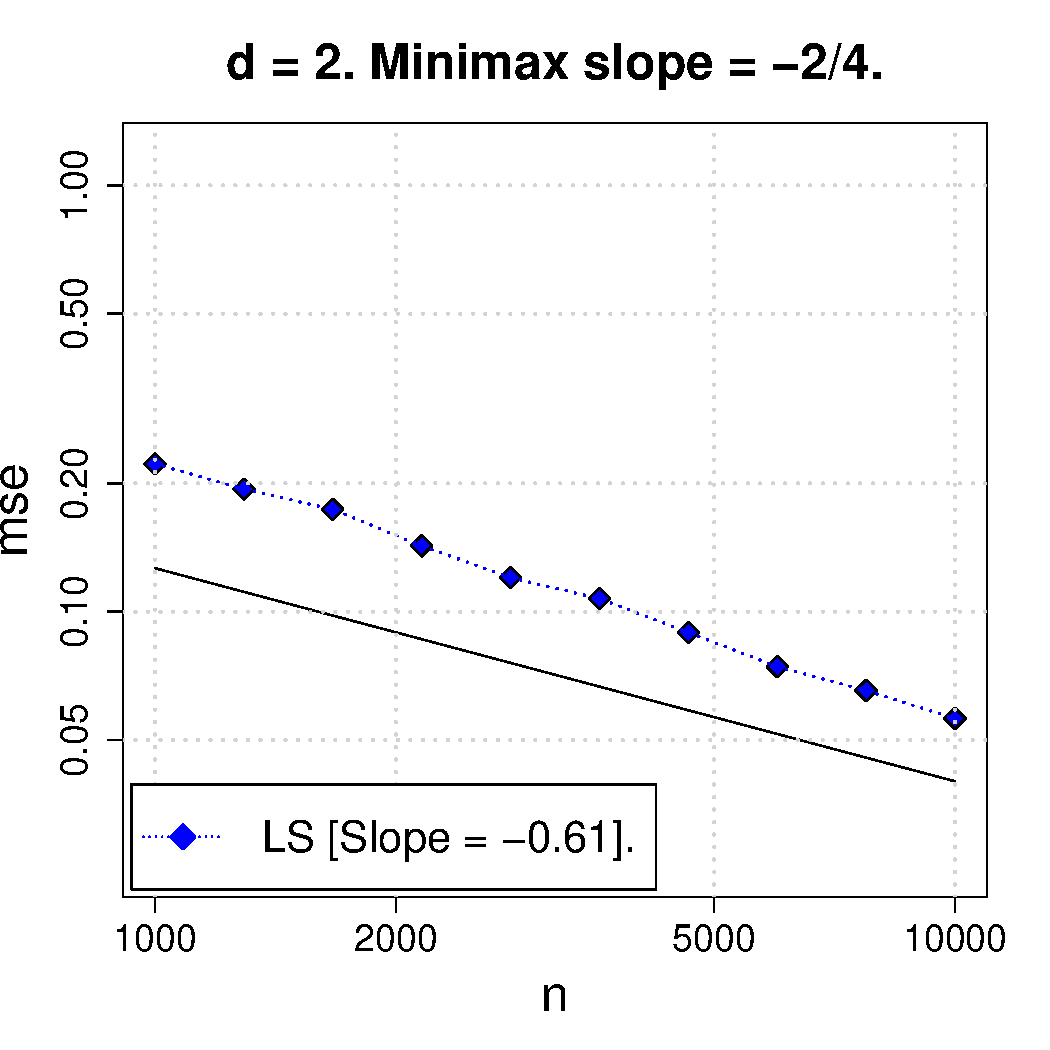
\includegraphics[width=.245\textwidth]{figures/cosine/mse_by_sample_size_2d.pdf}
	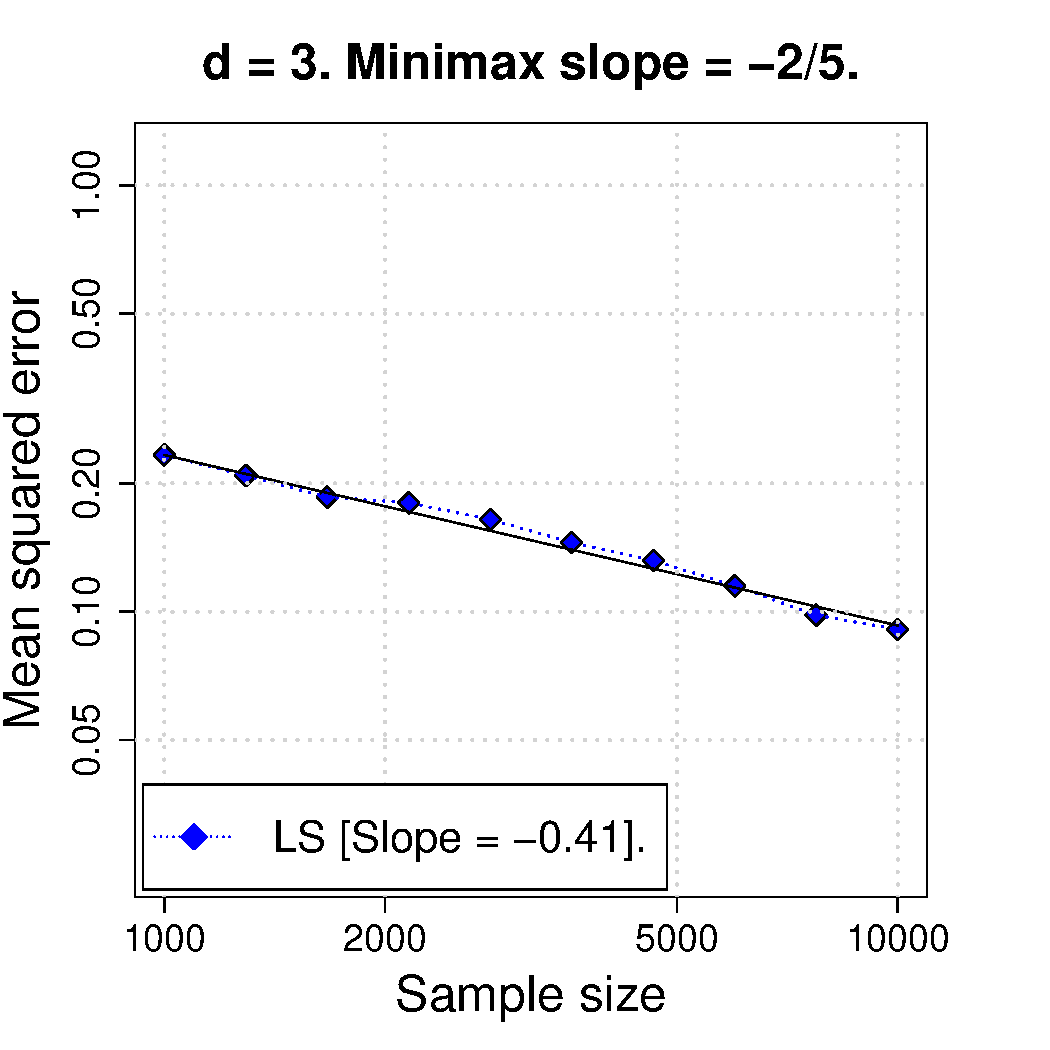
\includegraphics[width=.245\textwidth]{figures/cosine/mse_by_sample_size_3d.pdf} 
	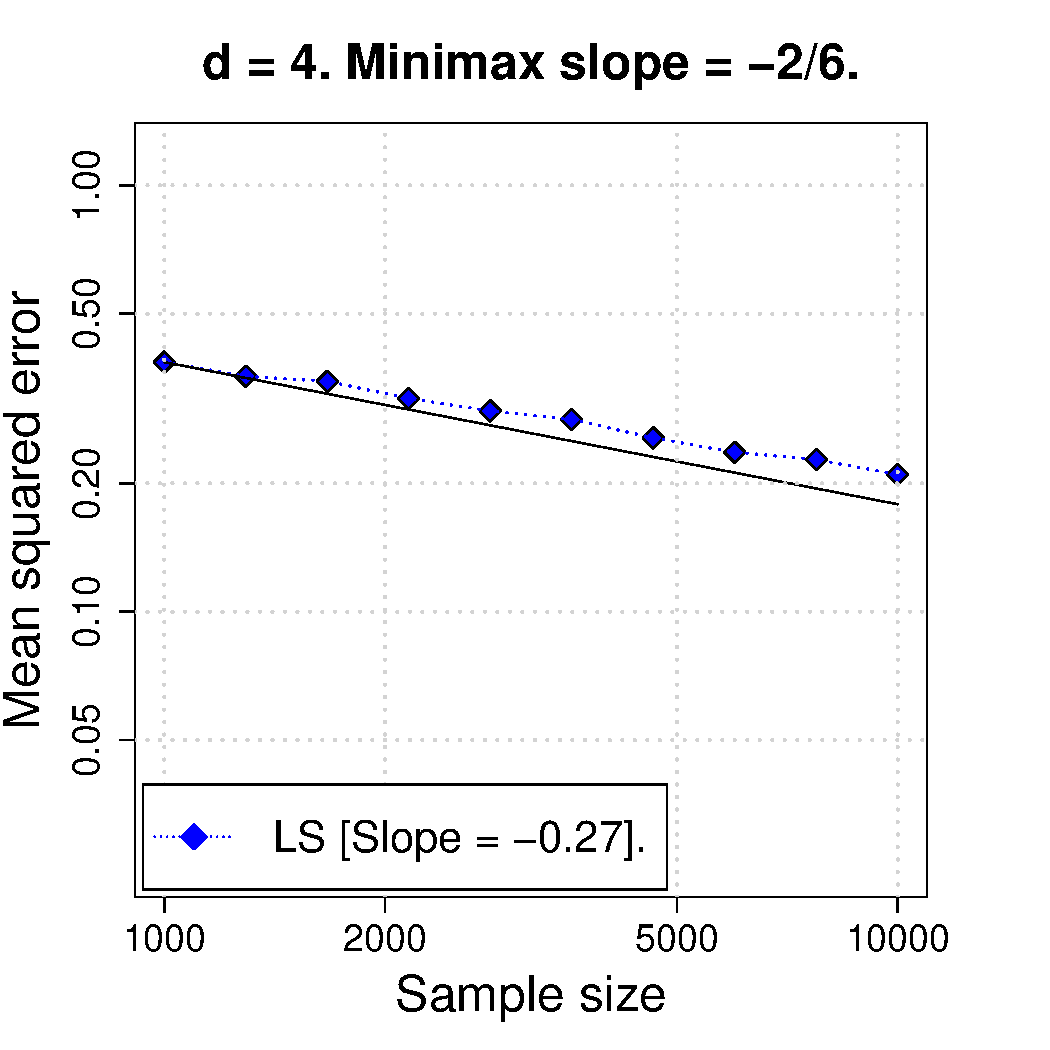
\includegraphics[width=.245\textwidth]{figures/cosine/mse_by_sample_size_4d.pdf}
	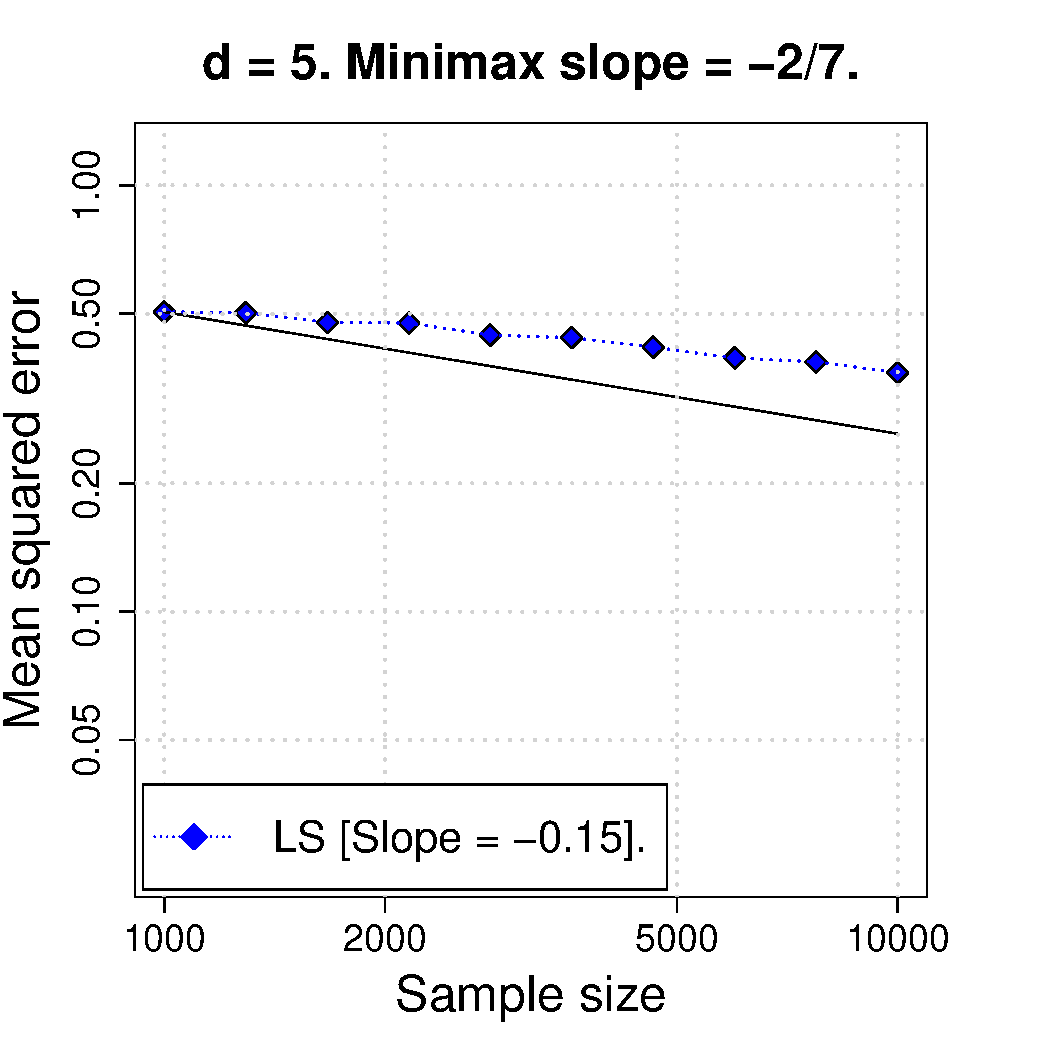
\includegraphics[width=.245\textwidth]{figures/cosine/mse_by_sample_size_5d.pdf}
	\caption{Mean squared error of Laplacian smoothing (\texttt{LS}) as a function of sample size $n$. Each plot is on the log-log scale, and the results are averaged over 5 repetitions, with Laplacian smoothing tuned for optimal average mean squared error. The black line shows the minimax rate (in slope only; the intercept is chosen to match the observed error).}
	\label{fig:fig1}
	% RJT: Alden, please verify that what I wrote about the intercept above is right. And if so, can you redo the black line for d = 2 so that the intercept matches better? Thanks. Oh and if you're already going to redo one of these plots, you can satisfy my unreasonably nitpicky brain and change the x- and y-axes on all of them to use words rather than symbols/acronyms: "Sample size" and "Mean squared error". 
	% AJG: Verified, and redone with requested changes.
\end{figure*}

\paragraph{Testing Error of Laplacian Smoothing.}

For $b \geq 1$, define a threshold \smash{$\wh{t}_b$} as
\begin{equation*}
\wh{t}_{b} = \frac{1}{n}\sum_{k = 1}^{n} \frac{1}{(\rho \lambda_k + 1)^2} + \frac{2b}{n}\sqrt{\sum_{k = 1}^{n} \frac{1}{(\rho \lambda_k + 1)^4}},
\end{equation*}
where we recall $\lambda_k$ is the $k$th smallest eigenvalue of \smash{$\Lap_{n,r}$}. The Laplacian smoothing test is then simply
\begin{equation*}
\wh{\varphi} = \1\bigl\{\wh{T} \leq \wh{t}_b\bigr\}.
\end{equation*} 
%(Clearly \smash{$\wh{\varphi}$} depends on $b$, but we suppress this notationally.) 
Here $b \geq 1$ is a tuning parameter selected by the user, with the choice driven by the tolerated Type I versus Type II error. In fact, the threshold \smash{$\wh{t}_b$} is precisely the right choice to control the Type I error of \smash{$\wh{\varphi}$}: we show in Appendix~\ref{sec:fixed_graph_error_bounds} that
\begin{equation}
\label{eqn:type_I_error}
\Ebb_0\bigl[\wh{\varphi}\bigr] \leq \frac{1}{b^2}.
\end{equation}
The next theorem shows that this test also has small Type II error, uniformly over all $f_0$ that are separated from $0$ by at least the critical radius given in \eqref{eqn:sobolev_space_testing_critical_radius}. For this to hold, we will require a tighter range of scalings for the graph radius $r$.
\begin{enumerate}[label=(R\arabic*)]
	\setcounter{enumi}{1}
	\item 
	\label{asmp:ls_kernel_radius_testing}
	For constants $C_0,c_0>0$, the neighborhood graph radius $r$ satisfies
	\begin{equation*}
	C_0\biggl(\frac{\log n}{n}\biggr)^{\frac{1}{d}} \leq r \leq c_0 \wedge M^{\frac{(d - 8)}{8 + 2d}} n^{\frac{d - 20}{32 + 8d}}.
	\end{equation*}
\end{enumerate}
We will also require that the radius of the Sobolev class not be too large. \\
%\sbcomment{What does the class have to do with graphs?}  \\
%\agcomment{Resolved.} \\
Precisely, we will require $M \leq M_{\max}(d)$, where we define
\begin{equation*}
M_{\max}(d) :=
\begin{cases*}
n^{1/8} & \textrm{$d = 1$} \\
n^{(4 - d)/(4d)} & \textrm{$d \geq 2$}.
\end{cases*}
\end{equation*}

We now give Theorem~\ref{thm:laplacian_smoothing_testing}, our main testing result.
\begin{theorem}
	\label{thm:laplacian_smoothing_testing}
	Given i.i.d.\ draws $(X_i,Y_i)$, $i=1,\ldots,n$ from \eqref{eqn:signal_plus_noise_model}, assume $f_0 \in H^1(\Xset,M)$ where $\Xset \subseteq \Rd$ with $d < 4$, and where $M \leq M_{\max}(d)$. Assume \ref{asmp:domain}, \ref{asmp:density} on the design distribution $P$, and assume \smash{$G_{n,r}$} is computed with a kernel $K$ satisfying \ref{asmp:kernel}. There are constants $N,C,c>0$ such that for any $n \geq N$, and any radius $r$ as in \ref{asmp:ls_kernel_radius_testing}, the Laplacian smoothing test \smash{$\wh{\varphi}$} based on the estimator \smash{$\wh{f}$} in \eqref{eqn:laplacian_smoothing}, with \smash{$\rho = (nr^{d + 2})^{-1} n^{-4/(4 + d)} M^{-8/(4 + d)}$}, satisfies the following: for all $b \geq 1$, and all $f_0$ such that
	\begin{equation}
	\label{eqn:laplacian_smoothing_testing}
	\bigl\|f_0\bigr\|_{\Leb^2(\Xset)}^2 \geq C b^2 M^{2d/(4 + d)} n^{-4/(4 + d)},
	\end{equation} 
	the Type II error is upper bounded by
	\begin{equation*}
	\Ebb_{f_0}\bigl[1 - \wh{\varphi} \bigr] \leq C\biggl(\frac{1}{b}\Bigl[1 + n^{-d/(4 + d)}M^{-2d/(4 + d)}\Bigr] + n\exp\bigl(-cnr^d\bigr)\biggr).
	\end{equation*}
\end{theorem}
\sbcomment{Personally, I wouldn't emphasize the Type II error so much in the Theorem (it is not tight and it's not an interesting quantity anyway), and write \eqref{eqn:laplacian_smoothing_testing} more directly as an upper bound on the critical radius (which is the interesting quantity). Otherwise you've introduced that terminology for no reason.}

Some remarks:
\begin{itemize}
	\item As mentioned earlier, Sobolev balls $H^1(\Xset,M)$ for $d \geq 4$ include quite irregular functions $f \not\in \Leb^4(\Xset)$. Proving tight lower bounds in this case is nontrivial, and as far as we understand such an analysis remains outstanding. On the other hand, if we explicitly assume that $f_0 \in \Leb^4(\Xset,M)$, then \citet{guerre02} show that the testing problem is characterized by a dimension-free lower bound $\epsilon^{2}(\Leb^4(\Xset,M)) \gtrsim n^{-1/2}$. Moreover, by estimating \smash{$\wh{f}$}, setting $\rho = 0$, the subsequent test \smash{$\wh{\varphi}$} will achieve (up to constants) this lower bound. That is, for any $f_0 \in \Leb^4(\Xset,M)$ such that \smash{$\|f_0\|_{\Leb^2(\Xset)}^2 \geq C b^2n^{-1/2}$}, we have both
	\begin{equation}
	\label{eqn:laplacian_smoothing_testing_low_smoothness}
	\Ebb_{f_0}\bigl[1 - \wh{\varphi}\bigr] \leq \frac{C(1 + M^4)}{b^2},
	\end{equation} 
	and \smash{$\Ebb_0[\wh{\varphi}] \leq 1/b^2$}. Note that the same results apply to \smash{$\wt{T}$}, since the thin-plate spline estimator \smash{$\wt{f}$} interpolates the responses $Y_1,\ldots,Y_n$ for $d>1$.
	\item To compute the data-dependent threshold \smash{$\wh{t}_b$}, one must know all of the eigenvalues $\lambda_1,\ldots,\lambda_n$. Computing all these eigenvalues is far more expensive (cubic-time) than computing \smash{$\wh{T}$} in the first place (nearly-linear-time). But in practice we would not recommend using \smash{$\wh{t}_b$} anyway, and would instead we make the standard recommendation to calibrate via a permutation test \citep{hoeffding1952}. Recent work \cite{kim2020minimax}, has shown that in a variety of closely related settings, calibration of a test statistic via the permutation test often retains minimax-optimal power, and we expect similar results to hold for the Laplacian smoothing-based test statistic.

\end{itemize}

\paragraph{More Discussion of Variational Analog.}

With some results in hand, let us pause to offer some explanation of why Laplacian smoothing can be optimal in settings where thin-plate splines are not even consistent. First, we elaborate on why this difference in performance is so surprising. As mentioned previously, the penalties in \eqref{eqn:laplacian_smoothing}, \eqref{eqn:thin_plate_spline} can be closely tied together: \citet{bousquet03} show that for $f \in C^2(\Xset)$, 
\begin{equation}
\label{eqn:seminorm_consistency}
\begin{aligned}
\lim \frac{1}{n^2 r^{d + 2}} f^\top \Lap_{n,r} f & = \int_{\Xset} f(x) \cdot \Delta_Pf(x) p(x) \,dx \\
& = \int_{\Xset} \|\nabla f(x)\|_2^2 p^2(x) \,dx.
\end{aligned}
\end{equation}
In the above, the limit is as $n \to \infty$ and $r \to 0$, $\Delta_P$ is the (weighted) Laplace-Beltrami operator
\begin{equation*}
\Delta_Pf := -\frac{1}{p} \dive\bigl(p^2\nabla f),
\end{equation*}
and the second equality follows using integration by parts.\footnote{Assuming $f$ satisfies e.g., Dirichlet boundary conditions.} To be clear, this argument does not formally imply that the Laplacian eigenmaps estimator $\wh{f}$ and the thin-plate spline estimator $\wt{f}$ are close (for one, note that \eqref{eqn:seminorm_consistency} holds for $f \in C^2(\Xset)$, whereas the optimization in \eqref{eqn:thin_plate_spline} considers a much broader set of continuous functions with weak derivatives in $\Leb^2(\Xset)$). But it does seem to suggest that the two estimators should behave somewhat similarly. 

Of course, we know this is not the case: \smash{$\wh{f}$} and \smash{$\wt{f}$} look very different when $d > 1$. What is driving this difference? The key point is that the discretization imposed by the graph $G_{n,r}$---which might seem problematic at first glance---turns out to be a blessing. The problem with~\eqref{eqn:thin_plate_spline} is that the class $H^1(\Xset)$, which fundamentally underlies the criterion, is far ``too big'' for $d > 1$. This is meant in various related senses. By the Sobolev embedding theorem, for $d>1$, the class $H^1(\Xset)$ does not continuously embed into any H\"{o}lder space; and in fact it does not even continuously embed into $C^0(\Xset)$. Thus we cannot really restrict the optimization to \emph{continuous} and weakly differentiable functions, as we could when $d=1$ (the smoothing spline case), without throwing out a substantial subset of functions in $H^1(\Xset)$. Even among continuous and differentiable functions $f$, as we explained previously, we can use ``bump'' functions (as in \citet{green93}) to construct $f$ that interpolates the pairs $(X_i,Y_i)$, $i=1,\ldots,n$ and achieves arbitrarily small penalty (and hence criterion) in \eqref{eqn:thin_plate_spline}. In this sense, any estimator resulting from solving \eqref{eqn:thin_plate_spline} will clearly be inconsistent. 

On the other hand, problem \eqref{eqn:laplacian_smoothing} is finite-dimensional. As a result \smash{$\wh{f}$} has far less capacity to overfit than does \smash{$\wt{f}$}, for any given sample size $n$. Discretization is not the only way to make the problem \eqref{eqn:thin_plate_spline} more tractable: for instance, one can replace the penalty \smash{$\int_{\Xset} \|\nabla f(x)\|_2^2 \,dx$} with a stricter choice like \smash{$\esssup_{x \in \Xset} \|\nabla f(x)\|_2$}, or conduct the optimization over some finite-dimensional linear subspace of $H^1(\Xset)$ (i.e., use a sieve). While these solutions do improve the statistical properties of \smash{$\wt{f}$} for $d > 1$ (see e.g., \citet{birge1993,birge1998,vandergeer2000}), Laplacian smoothing is generally speaking much simpler and more computationally friendly. In addition, the other approaches are usually specifically tailored to the domain $\Xset$, in stark contrast to~\smash{$\wh{f}$}.

\paragraph{Overview of Analysis.}

The comparison with thin-plate splines highlights some surprising differences between \smash{$\wh{f}$} and \smash{$\wt{f}$}. Such differences also preclude us from analyzing \smash{$\wh{f}$} by, say, using \eqref{eqn:seminorm_consistency} to establish a coupling between \smash{$\wh{f}$} and \smash{$\wt{f}$}---we know this cannot work, because we would like to prove meaningful error bounds on \smash{$\wh{f}$} in regimes where no such bounds exist for \smash{$\wt{f}$}.

Instead we take a different approach, and directly analyze the error of \smash{$\wh{f}$} and \smash{$\wh{T}$} using a bias-variance decomposition (conditional on $X_1,\ldots,X_n$). A standard calculation shows that
\begin{equation*}
\bigl\|\wh{f} - f_0\bigr\|_n^2 \leq \underbrace{\vphantom{\sum_{k=1}^n}\frac{2\rho}{n} \bigl(f_0^\top \Lap_{n,r} f_0\bigr)}_{\textrm{bias}} + \underbrace{\frac{10}{n} \sum_{k = 1}^{n} \frac{1}{(\rho \lambda_k + 1)^2}}_{\textrm{variance}},
\end{equation*}
and likewise that $\wh{\varphi}$ has high power whenever
\begin{equation*}
\bigl\|f_0\bigr\|_n^2 \geq \underbrace{\vphantom{\sqrt{\sum_{k=1}^n}}\frac{2\rho}{n} \bigl(f_0^\top \Lap_{n,r} f_0\bigr)}_{\textrm{bias}} + \underbrace{\frac{4b}{n} \sqrt{\sum_{k = 1}^{n} \frac{1}{(\rho \lambda_k + 1)^4}}}_{\textrm{variance}}.
\end{equation*}
The bias and variance terms are each functions of the random graph \smash{$G_{n,r}$}, and hence are themselves random. To upper bound them, we build on some recent works \citep{burago2014,trillos2019,calder2019} regarding the consistency of neighborhood graphs to establish the following lemmas. These lemmas assume \ref{asmp:domain}, \ref{asmp:density} on the design distribution $P$, and \ref{asmp:kernel} on the kernel used to compute the neighborhood graph \smash{$G_{n,r}$}. 

\begin{lemma}
	\label{lem:graph_sobolev_seminorm}
	There are constants $N,C_2 > 0$ such that for $n \geq N$, $r \leq c_0$, and $f \in H^1(\Xset)$, with probability at least $1 - \delta$, it holds that
	\begin{equation}
	\label{eqn:graph_sobolev_seminorm}
	f^\top \Lap_{n,r} f \leq \frac{C_2}{\delta} n^2 r^{d + 2} |f|_{H^1(\Xset)}^2.
	\end{equation}
\end{lemma}

\begin{lemma}
	\label{lem:neighborhood_eigenvalue} 
	There are constants $N,C_1,C_3,c_1,c_3 > 0$ such that for $n \geq N$ and $C_0(\log n/n)^{1/d} \leq r \leq c_0$, with probability at least $1 - C_1n\exp(-c_1nr^d)$, it holds that
	\begin{equation}
	\label{eqn:neighborhood_eigenvalue}
	c_3A_{n,r}(k) \leq \lambda_k \leq C_3A_{n,r}(k), ~~\textrm{for $2 \leq k \leq n$},
	\end{equation}
	where \smash{$A_{n,r}(k) = \min\{nr^{d + 2}k^{2/d},nr^d\}$}.
\end{lemma}

Lemma~\ref{lem:graph_sobolev_seminorm} gives a direct upper bound on the bias term. Lemma~\ref{lem:neighborhood_eigenvalue} leads to a sufficiently tight upper bound on the variance term whenever the radius $r$ is sufficiently small; precisely, when $r$ is upper bounded as in \ref{asmp:ls_kernel_radius_estimation} for estimation, or \ref{asmp:ls_kernel_radius_testing} for testing. The parameter $\rho$ is then chosen to minimize the sum of these upper bounds on bias and variance, as usual, and some straightforward calculations give Theorems~\ref{thm:laplacian_smoothing_estimation1}-\ref{thm:laplacian_smoothing_testing}.\\
%\sbcomment{Should probably say something about the rest of the proof, i.e. is it straightforward to put these together to get the two Theorems?} \\
%\agcomment{Attempted to resolve.}

It may be useful to give one more perspective on our approach. A common strategy in analyzing penalized least squares estimators is to assume two properties: first, that the regression function $f_0$ lies in (or near) a ball defined by the penalty operator; second, that this ball is reasonably small, e.g., as measured by metric entropy, or Rademacher complexity, etc. In contrast, in Laplacian smoothing, the penalty induces a ball
\begin{equation*}
H^1(G_{n,r},M) := \{f: f^\top \Lap_{n,r} f \leq M^2\}
\end{equation*}
that is data-dependent and random, and so we do not have access to either of the aforementioned properties a priori, and instead, must prove they hold with high probability. In this sense, our analysis is different than the typical one in nonparametric regression.

\section{Manifold Adaptivity}
\label{sec:manifold_adaptivity}

The minimax rates $n^{-2/(2 + d)}$ and $n^{-4/(4 + d)}$, in estimation and testing, suffer from the curse of dimensionality. However, in practice it can be often reasonable to assume a \emph{manifold hypothesis}: that the data $X_1,\ldots,X_n$ lie on a manifold $\Xset$ of $\Rd$ that has intrinsic dimension $m < d$. Under such an assumption, it is known \citep{bickel2007,ariascastro2018} that the optimal rates over $H^1(\Xset)$ are now $n^{-2/(2 + m)}$ (for estimation) and $n^{-4/(4 + m)}$ (for testing), which are much faster than the full-dimensional error rates when $m \ll d$. \sbcomment{I might point out that the Arias-Castro result is for density testing over Holder spaces, and that technically rates for regression testing on manifolds for Sobolev spaces are your contribution.}

% RJT: Again, would venture a guess that these are stated results for Holder classes, not Sobolev classes. So same comment as before, as when we referenced Tsybakov. Just checking my understanding ... not sure it's worth changing this at this point. 

On the other hand, a theory has been developed \citep{niyogi2008finding,belkin03,belkin05,niyogi2013,balakrishnan2012minimax,balakrishnan2013cluster} establishing that the neighborhood graph $G_{n,r}$ can ``learn'' the manifold $\Xset$ in various senses, so long as $\Xset$ is locally linear. We contribute to this line of work by showing that under the manifold hypothesis, Laplacian smoothing achieves the tighter minimax rates over $H^1(\Xset)$.

\paragraph{Error Rates Assuming the Manifold Hypothesis.}

The conditions and results presented here will be largely similar to the previous ones, except with the ambient dimension $d$ replaced by the intrinsic dimension $m$. For the remainder, we assume the following.
\begin{enumerate}[label=(P\arabic*)]
	\setcounter{enumi}{2}
	\item 
	\label{asmp:domain_manifold}
	$P$ is supported on a compact, connected, smooth manifold $\Xset$ embedded in $\Rd$, of dimension $m \leq d$. The manifold is without boundary and has positive reach \citep{federer1959}.
	\item 
	\label{asmp:density_manifold} 
	$P$ admits a density $p$ with respect to the volume form of $\Xset$ such that 
	\begin{equation*}
	0 < p_{\min} \leq p(x) \leq p_{\max} < \infty, ~~\textrm{for all $x \in \Xset$}. 
	\end{equation*}
	Additionally, $p$ is Lipschitz on $\Xset$, with Lipschitz constant $L_p$.
\end{enumerate}

Under the assumptions \ref{asmp:domain_manifold}, \ref{asmp:density_manifold}, and \ref{asmp:kernel}, and for a suitable range of $r$, the error bounds on the estimator \smash{$\wh{f}$} and test \smash{$\wh{\varphi}$} will depend on $m$ instead of $d$. 
\begin{enumerate}[label=(R\arabic*)]
	\setcounter{enumi}{3}
	\item 
	\label{asmp:ls_kernel_radius_estimation_manifold}
	For constants $C_0,c_0>0$, the neighborhood graph radius $r$ satisfies 
	\begin{equation*}
	C_0\biggl(\frac{\log n}{n}\biggr)^{\frac{1}{m}} \leq r \leq c_0 \wedge  M^{\frac{(m - 4)}{(4 + 2m)}} n^{\frac{-3}{(4 + 2m)}}.
	\end{equation*}
\end{enumerate}

\begin{theorem}
	\label{thm:laplacian_smoothing_estimation_manifold}
	As in Theorem \ref{thm:laplacian_smoothing_estimation1}, but where $\Xset \subseteq \Rd$ is a manifold with intrinsic dimension $m < 4$, the design distribution $P$ obeys \ref{asmp:domain_manifold}, \ref{asmp:density_manifold}, and $M \leq n^{1/m}$. There are constants $N,C,C_1,c,c_1>0$ (not depending on $f_0$) such that for any \smash{$n \geq N$}, and any $r$ as in \ref{asmp:ls_kernel_radius_estimation_manifold}, the Laplacian smoothing estimator \smash{$\wh{f}$} in \eqref{eqn:laplacian_smoothing}, with \smash{$L = L_{n,r}$} and \smash{$\rho = M^{-4/(2 + m)} (nr^{m + 2})^{-1} n^{-2/(2 + m)}$}, satisfies
	\begin{equation*}
	\bigl\|\wh{f} - f_0\bigr\|_n^2 \leq \frac{C}{\delta} M^{2m/(2 + m)} n^{-2/(2 + m)},
	\end{equation*}
	with probability at least $1 - \delta -  C_1 n\exp(-cnr^m) - \exp(-c(M^2n)^{m/(2+m)})$.
	% RJT: Alden, please verify that what I wrote is correct.
	% AJG: Verified.
\end{theorem}
In a similar vein, we obtain results for manifold adaptive testing under the following condition on the graph radius parameter:
\begin{enumerate}[label=(R\arabic*)]
	\setcounter{enumi}{4}
	\item 
	\label{asmp:ls_kernel_radius_testing_manifold}
	For constants $C_0,c_0>0$, the neighborhood graph radius $r$ satisfies 
	\begin{equation*}
	C_0\biggl(\frac{\log n}{n}\biggr)^{\frac{1}{m}} \leq r \leq c_0 \wedge M^{\frac{(m - 8)}{8 + 2m}} n^{\frac{m - 20}{32 + 8m}}.
	\end{equation*}
\end{enumerate}

\begin{theorem}
	\label{thm:laplacian_smoothing_testing_manifold}
	As in Theorem \ref{thm:laplacian_smoothing_testing}, but where $\Xset \subseteq \Rd$ is a manifold with intrinsic dimension $m < 4$, $M \leq M_{\max}(m)$, and the design distribution $P$ obeys \ref{asmp:domain_manifold}, \ref{asmp:density_manifold}.
	There are constants $N,C,c>0$ such that for any $n \geq N$, and any $r$ as in \ref{asmp:ls_kernel_radius_testing_manifold}, the Laplacian smoothing test \smash{$\wh{\varphi}$} based on the estimator \smash{$\wh{f}$} in \eqref{eqn:laplacian_smoothing}, with \smash{$\rho = (nr^{m + 2})^{-1} n^{-4/(4 + m)} M^{-8/(4 + m)}$}, satisfies the following: for all $b \geq 1$, and $f_0$ such that
	\begin{equation}
	\label{eqn:laplacian_smoothing_testing_manifold}
	\bigl\|f_0\bigr\|_{\Leb^2(\Xset)}^2 \geq C b^2 M^{2m/(4 + m)} n^{-4/(4 + m)},
	\end{equation} 
	the Type II error is upper bounded by
	\begin{equation*}
	\Ebb_{f_0}\bigl[1 - \wh{\varphi} \bigr] \leq C\biggl(\frac{1}{b}\Bigl[1 + n^{-m/(4 + m)}M^{-2m/(4 + m)}\Bigr] + n\exp\bigl(-cnr^m\bigr)\biggr).
	\end{equation*}
	% RJT: Alden, please verify that what I wrote is correct.
	% AJG: Verified.
\end{theorem}
\sbcomment{Same comment as before on what to emphasize.}

The proof of Theorems \ref{thm:laplacian_smoothing_estimation_manifold} and \ref{thm:laplacian_smoothing_testing_manifold} proceeds in a similar manner to that of Theorems \ref{thm:laplacian_smoothing_estimation1} and \ref{thm:laplacian_smoothing_testing}. The key difference is that in the manifold setting, the equations \eqref{eqn:graph_sobolev_seminorm} and \eqref{eqn:neighborhood_eigenvalue} used to upper bound bias and variance will hold with $d$ replaced by $m$.

We emphasize that little about $\Xset$ needs be known for Theorems~\ref{thm:laplacian_smoothing_estimation_manifold} and \ref{thm:laplacian_smoothing_testing_manifold} to hold. Indeed, all that is needed is the intrinsic dimension $m$, to properly tune $r$ and $\rho$ (from a theoretical point of view), and otherwise \smash{$\wh{f}$} and \smash{$\wh{\varphi}$} are computed without regard to $\Xset$. In contrast, the penalty in \eqref{eqn:thin_plate_spline} would have to be specially tailored to work in this setting, revealing another advantage of the discrete approach over the variational one.

\section{Discussion}
\label{sec:discussion}

We have shown that Laplacian smoothing, computed over a neighborhood graph, can be optimal for both estimation and goodness-of-fit testing over Sobolev spaces. There are many extensions worth pursuing, and several have already been mentioned. We conclude by mentioning a couple more. In practice, it is more common to use a $k$-nearest-neighbor (kNN) graph than a neighborhood graph, due to the guaranteed connectivity and sparsity of the former; we suspect that by building on the work of \citet{calder2019}, one can show that our main results all hold under the kNN graph as well. In another direction, one can also generalize Laplacian smoothing by replacing the penalty \smash{$f^\top \Lap_{n,r} f$} with \smash{$f^\top \Lap_{n,r}^{s} f$}, for an integer $s > 1$. The hope is that this would then achieve minimax optimal rates over the higher-order Sobolev class $H^s(\Xset)$. % In the very special case of $k = 2$ and $d \leq 2$, we can show that this is indeed the case, but the general story--for all combinations of $k$ and $d$---remains beyond our reach. 
%\sbcomment{Not a huge fan of using $k$ in adjacent lines to refer to completely different things.}\\
%\agcomment{Resolved.}

\subsection*{Acknowledgements}
AG and RJT were supported by ONR grant N00014-20-1-2787. AG and SB were supported by NSF grants DMS-1713003 and CCF-1763734.

\bibliographystyle{unsrtnat}
\bibliography{../../../graph_regression_bibliography} 

\appendix

\noindent 

\section{Graph-dependent error bounds}
\label{sec:fixed_graph_error_bounds}
In this section, we adopt the fixed design perspective; or equivalently, condition on $X_i = x_i$ for $i = 1,\ldots,n$. Let $G = \bigl([n],W\bigr)$ be a fixed graph on $\{1,\ldots,n\}$ with Laplacian matrix $L = \sum_{k = 1}^{n}\lambda_k v_k v_k^{\top}$; the eigenvectors have unit empirical norm, $\|v_k\|_n^2 = 1$. The randomness thus all comes from the responses 
\begin{equation}
\label{eqn:fixed_graph_regression_model}
Y_i = f_{0}(x_i) + w_i
\end{equation}
where the noise variables $w_i$ are independent $N(0,1)$. In the rest of this section, we will mildly abuse notation and write $f_0 = (f_0(x_1),\ldots,f_0(x_n)) \in \Reals^n$. We will also write ${\bf Y} = (Y_1,\ldots,Y_n)$.

\subsection{Upper bound on Estimation Error of Laplacian Eigenmaps}

\begin{lemma}
	\label{lem:fixed_graph_estimation}
	For any integer $s > 0$, and any integer $0 \leq K \leq n$, the Laplacian eigenmaps estimator $\wh{f}$ of~\eqref{eqn:laplacian_eigenmaps_estimator} satisfies
	\begin{equation}
	\label{eqn:fixed_graph_estimation}
	\|\wh{f} - f_0\|_n^2 \leq \frac{\dotp{L^sf_0}{f_0}_n}{\lambda_{K + 1}^s} + \frac{5K}{n};
	\end{equation}
	this is guaranteed if $K = 0$, and otherwise holds with probability at least $1 - \exp(-K)$ if $1 \leq K \leq n$. 
\end{lemma}
\paragraph{Proof (of Lemma~\ref{lem:fixed_graph_estimation}).}
	By the triangle inequality,
	\begin{equation}
	\label{pf:fixed_graph_estimation_1}
	\|\wh{f} - f_0\|_n^2 \leq 2\Bigl(\|\mathbb{E}\wh{f} - f_0\|_n^2 + \|\wh{f} - \mathbb{E}\wh{f}\|_n^2\Bigr).
	\end{equation}
	The first term in~\eqref{pf:fixed_graph_estimation_1} (approximation error) is non-random, since the design is fixed. The expectation $\mathbb{E}\wh{f} = \sum_{k = 1}^{K} \dotp{v_k}{f_0}_n v_k$, so that
	\begin{equation*}
	\|\mathbb{E}\wh{f} - f_0\|_n^2 = \Bigl\|\sum_{k = K + 1}^{n} \dotp{v_k}{f_0}_n v_k\Bigr\|_n^2 = \sum_{k = K + 1}^n \dotp{v_k}{f_0}_n^2.
	\end{equation*}
	In the above, the last equality relies on the fact that $v_k$ are orthonormal in $L^2(P_n)$. Using the fact that the eigenvalues are in increasing order, we obtain
	\begin{equation*}
	\sum_{k = K + 1}^n \dotp{v_k}{f_0}_n^2 \leq \frac{1}{\lambda_{K + 1}^s} \sum_{k = K + 1}^n \lambda_k^s \dotp{v_k}{f_0}_n^2 \leq \frac{\dotp{L^sf_0}{f_0}_n}{\lambda_{K + 1}^s}.
	\end{equation*}
	
	If $K = 0$, $\wh{f} = \Ebb{\wh{f}} = 0$, and the second term in~\eqref{pf:fixed_graph_estimation_1} is $0$. Otherwise the second   in~\eqref{pf:fixed_graph_estimation_1} (estimation error) is random. Observe that $\dotp{v_k}{\varepsilon}_n \overset{d}{=} Z_k/\sqrt{n}$, where $(Z_1,\ldots,Z_n) \sim N(0,I_{n \times n})$. Again using the orthonormality of the eigenvectors $v_k$, we have
	\begin{equation*}
	\|\wh{f} - \mathbb{E}\wh{f}\|_n^2 = \sum_{k = 1}^{K} \dotp{v_k}{\varepsilon}_n^2 \overset{d}{=} \frac{1}{n}\sum_{k = 1}^{K} Z_k^2.
	\end{equation*}
	Thus $\|\wh{f} - \mathbb{E}\wh{f}\|_n^2$ is equal to $1/n$ times a $\chi^2$ distribution with $K$ degrees of freedom. Consequently, it follows from a result of \citep{laurent00} that
	\begin{equation*}
	\Pbb\biggl(\|\wh{f} - \mathbb{E}\wh{f}\|_n^2 \geq \frac{K}{n} + 2\frac{\sqrt{K}}{n}\sqrt{t} + \frac{2t}{n}\biggr) \leq \exp(-t).
	\end{equation*}
	Setting $t = K$ completes the proof of the lemma.

\subsection{Upper bound on Testing Error of Laplacian Eigenmaps}

Let $\wh{T} = \sum_{k = 1}^{K} \dotp{{\bf Y}}{v_k}_n^2$, and let $\varphi = \1\{\wh{T} \geq t_a\}$. In the following Lemma, we upper bound the Type I and Type II error of the test $\varphi$.

\begin{lemma}
	\label{lem:fixed_graph_testing}
	Suppose we observe $(Y_1,x_1),\ldots,(Y_n,x_n)$ according to~\eqref{eqn:fixed_graph_regression_model}.
	\begin{itemize}
		\item If $f_0 = 0$, then $\Ebb_0[\varphi] \leq a$.
		\item Suppose $f_0 \neq 0$ satisfies
		\begin{equation}
		\label{eqn:fixed_graph_testing_critical_radius}
		\|f_0\|_n^2 \geq \frac{\dotp{L^sf_0}{f_0}_n}{\lambda_{K + 1}^s} + \frac{\sqrt{2K}}{n}\biggl[2\sqrt{\frac{1}{a}} + \sqrt{\frac{2}{b}} + \frac{32}{bn}\biggr],
		\end{equation}
		for some $s \in \mathbb{N}\setminus \{0\}$. Then $\Ebb_{f_0}[1 - \phi] \leq b$.
	\end{itemize}
\end{lemma}
\paragraph{Proof (of Lemma~\ref{lem:fixed_graph_testing}).}
We first compute the expectation and variance of $\wh{T}$, then apply Chebyshev's inequality to upper bound the Type I and Type II error.

\underline{\emph{Expectation}.}
Recall that $\wh{T} = \sum_{k = 1}^{K} \dotp{Y}{v_k}_n^2$. Expanding the square gives
\begin{equation*}
\Ebb[\wh{T}] = \sum_{k = 1}^{K} \Ebb[\dotp{Y}{v_k}_n^2] = \sum_{k = 1}^{K} \dotp{f_0}{v_k}_n^2 + \Ebb[2\dotp{f_0}{v_k}_n\dotp{\varepsilon}{v_k}_n + \dotp{\varepsilon}{v_k}_n^2] = \frac{K}{n} + \sum_{k = 1}^{K} \dotp{f_0}{v_k}_n^2.
\end{equation*}
Thus $\Ebb[\wh{T}] - t_a = \sum_{k = 1}^{K} \dotp{f_0}{v_k}_n^2 - \sqrt{2K}/n \cdot \sqrt{1/a}$. Furthermore, it is a consequence of~\eqref{eqn:fixed_graph_testing_critical_radius} that 
\begin{equation}
\label{pf:fixed_graph_testing_1}
\sum_{k = 1}^{K} \dotp{f_0}{v_k}_n^2 - \frac{\sqrt{2K}}{n}\sqrt{1/a} \geq \|f_0\|_n^2 - \frac{\dotp{L^sf_0}{f_0}_n}{\lambda_{K + 1}^s} - \frac{\sqrt{2K}}{n}\sqrt{1/a} \geq \frac{\sqrt{2K}}{n}\biggl[\sqrt{\frac{1}{a}} + \sqrt{\frac{2}{b}} + \frac{32}{bn}\biggr].
\end{equation} 

\underline{\emph{Variance}.}
Recall from the proof of Lemma~\ref{lem:fixed_graph_estimation} that $\dotp{\varepsilon}{v_k}_n \overset{d}{=} Z_k/\sqrt{n}$ for $(Z_1,\ldots,Z_n) \sim N(0,I_{n \times n})$. Expanding the square, and recalling that $\Cov[Z,Z^2] = 0$ for Gaussian random variables, we have that
\begin{equation*}
\Var\bigl[\dotp{{\bf Y}}{v_k}_n^2\bigr] = \Var\biggl[\frac{2}{n}\dotp{f_0}{v_k}_nZ_k + \frac{2}{n^2}Z_k^2\biggr] = \frac{4\dotp{f_0}{v_k}_n^2}{n} + \frac{2}{n^2}.
\end{equation*}
Moreover, since $\Cov[Z_k^2,Z_{\ell}^2] = 0$ for each $k = 1,\ldots,K$, we see that
\begin{equation*}
\Var\bigl[\wh{T}\bigr] = \sum_{k = 1}^{K} \Var\bigl[\dotp{{\bf Y}}{v_k}_n^2\bigr] = \frac{2K}{n^2} + \sum_{k = 1}^{K}\frac{4\dotp{f_0}{v_k}_n^2}{n}.
\end{equation*}

\underline{\emph{Bounds on Type I and Type II error}.}
The upper bound on Type I error follows immediately from Chebyshev's inequality. 

The upper bound on Type II error also follows from Chebyshev's inequality. We observe that~\eqref{eqn:fixed_graph_testing_critical_radius} implies $\Ebb_{f_0}[\wh{T}] = t_a$, and apply Chebyshev's inequality to deduce
\begin{equation*}
\Pbb_{f_0}\bigl(\wh{T} < t_a\bigr) \leq \Pbb_{f_0}\Bigl(|\wh{T} - \Ebb_{f_0}[\wh{T}]|^2 > |\Ebb_{f_0}[\wh{T}] - t_a|^2\Bigr) \leq \frac{\Var\bigl[\wh{T}\bigr]}{\bigl[\Ebb_{f_0}[\wh{T}] - t_a\bigr]^2} = \frac{2K/n^2 + 4/n\sum_{k = 1}^{K}\dotp{f_0}{v_k}_n^2}{\bigl[\Ebb_{f_0}[\wh{T}] - t_a\bigr]^2}.
\end{equation*}
Thus we have upper bounded the Type II error by the sum of two terms, each of which are no more than $1/(2b)$, as we now show. For the first term, after noting that~\eqref{pf:fixed_graph_testing_1} implies $\Ebb_{f_0}[\wh{T}] - t_a \geq \sqrt{2K}/n \cdot \sqrt{2/b}$, the upper bound follows:
\begin{equation*}
\frac{2K/n^2}{\bigl[\Ebb_{f_0}[\wh{T}] - t_a\bigr]^2} \leq \frac{b}{2}.
\end{equation*}
On the other hand, for the second term we use~\eqref{pf:fixed_graph_testing_1} in two ways: first to conclude that $\Ebb_{f_0}[\wh{T}] - t_a \geq 1/2 \cdot \sum_{k = 1}^{K}\dotp{f_0}{v_k}_n^2$, and second to obtain
\begin{equation*}
\frac{4\sum_{k = 1}^{K}\dotp{f_0}{v_k}_n^2}{n\bigl[\Ebb_{f_0}[\wh{T}] - t_a\bigr]^2} \leq \frac{4\sum_{k = 1}^{K}\dotp{f_0}{v_k}_n^2}{n\bigl(\sum_{k = 1}^{K}\dotp{f_0}{v_k}_n^2/2\bigr)^2} \leq \frac{16}{n\sum_{k = 1}^{K}\dotp{f_0}{v_k}_n^2} \leq \frac{b}{2}.
\end{equation*}

\section{Graph Sobolev semi-norm, flat Euclidean domain}
\label{sec:graph_quadratic_form_euclidean}
In this section we prove Proposition~\ref{prop:graph_seminorm_ho}. The proposition will follow from several intermediate results.
\begin{enumerate}
	\item~In Section~\ref{subsec:decomposition_graph_seminorm}, we show that
	\begin{equation}
	\label{pf:graph_seminorm_ho_1}
	\dotp{L_{n,\varepsilon}^sf}{f}_n \leq \frac{1}{\delta} \dotp{L_{P,\varepsilon}^sf}{f}_{P} + \frac{C\varepsilon^2}{\delta n\varepsilon^{2 + d}}M^2.
	\end{equation}
	with probability at least $1 - 2\delta$. 
	
	We term the first term on the right hand side the \emph{non-local Sobolev semi-norm}, as it is a kernelized approximation to the Sobolev semi-norm $\dotp{\Delta_P^sf}{f}_{P}$. The second term on the right hand side is a pure bias term, which as we will see is negligible compared to the non-local Sobolev semi-norm as long as $\varepsilon \ll n^{-1/(2(s -1 + d))}$. 
	\item~In Section~\ref{subsec:approximation_error_nonlocal_laplacian}, we show that when $x$ is sufficiently in the interior of $\mc{X}$, then $L_{P,\varepsilon}^kf(x)$ is a good approximation to $\Delta_P^kf(x)$, as long as $f \in H^{s}(\mc{X})$ and $p \in C^{s - 1}(\mc{X})$ for some $s \geq 2k + 1$. 
	\item~In Section~\ref{subsec:boundary_behavior_nonlocal_laplacian}, we show that when $x$ is sufficiently near the boundary of $\mc{X}$, then $L_{P,\varepsilon}^kf(x)$ is close to $0$, as long as $f \in H_0^{s}(\mc{X})$ for some $s > 2k$.
	\item~In Section~\ref{subsec:estimate_nonlocal_seminorm}, we use the results of the preceding two sections to show that if $f \in H_0^s(\mc{X};M)$ and $p \in C^{s - 1}(\mc{X})$, there exists a constant $C$ which does not depend on $f$ such that
	\begin{equation}
	\label{pf:graph_seminorm_ho_2}
	\dotp{L_{P,\varepsilon}^sf}{f}_{P} \leq CM^2.
	\end{equation}
\end{enumerate}
Finally, in Section~\ref{subsec:integrals} we provide some assorted estimates used in Sections~\ref{subsec:decomposition_graph_seminorm}. 

\paragraph{Proof (of Proposition~\ref{prop:graph_seminorm_ho}).}
Proposition~\ref{prop:graph_seminorm_ho} follows immediately from~\eqref{pf:graph_seminorm_ho_1} and~\eqref{pf:graph_seminorm_ho_2}. \qed

One note regarding notation: suppose a function $g \in H^{\ell}(U)$, where $\ell \in \mathbb{N}$ and $U$ is an open set. Let $V$ be another open set, compactly contained within $U$. Then we will use the notation $g \in H^{\ell}(V)$ to mean that the restriction $\restr{g}{V}$ of $g$ to $V$ belongs to $H^{\ell}(V)$.

\subsection{Decomposition of graph Sobolev semi-norm}
\label{subsec:decomposition_graph_seminorm}

In Lemma~\ref{lem:graph_seminorm_bias}, we decompose the graph Sobolev semi-norm (a V-statistic) into an unbiased estimate of the non-local Sobolev semi-norm (a U-statistic), and a pure bias term. We establish that the pure bias term will be small (in expectation) relative to the U-statistic whenever $\varepsilon$ is sufficiently small.
\begin{lemma}
	\label{lem:graph_seminorm_bias}
	For any $f \in L^2(\mc{X})$, the graph Sobolev semi-norm satisfies
	\begin{equation}
	\label{eqn:graph_seminorm_bias_1}
	\dotp{L_{n,\varepsilon}^sf}{f}_{n} = U_{n,\varepsilon}^{(s)}(f) + B_{n,\varepsilon}^{(s)}(f),
	\end{equation}
	such that $\mathbb{E}[U_{n,\varepsilon}^{(s)}(f)] = (n - s - 1)!/n! \cdot \dotp{L_{P,\varepsilon}^sf}{f}_P$. If additionally $f \in H^1(\mc{X};M)$ and $\varepsilon \geq n^{-1/d}$, then the bias term $B_{n,\varepsilon}^{(s)}(f)$ satisfies
	\begin{equation}
	\label{eqn:graph_seminorm_bias_2}
	\mathbb{E}\bigl[|B_{n,\varepsilon}^{(s)}(f)|\bigr] \leq \frac{C\varepsilon^2}{\delta n\varepsilon^{2 + d}}M^2.
	\end{equation}
\end{lemma}
Then~\ref{pf:graph_seminorm_ho_1} follows immediately from Lemma~\ref{lem:graph_seminorm_bias}, by Markov's inequality.
\paragraph{Proof (of Lemma~\ref{lem:graph_seminorm_bias}).}
We begin by introducing some notation. We will use bold notation $\bj = (j_1,\ldots,j_s)$ for a vector of indices where $j_i \in [n]$ for each $i$. We write $[n]^s$ for the collection of all such vectors, and $(n)^s$ for the subset of such vectors with no repeated indices. Finally, we write $D_if$ for a kernelized difference operator,
\begin{equation*}
D_if(x) := \bigl(f(x) - f(X_i)\bigr) \eta\biggl(\frac{\|X_i - x\|}{\varepsilon}\biggr),
\end{equation*}
and we let $D_{\bj}f(x) := \bigl(D_{j_1}\circ \cdots \circ D_{j_s}f\bigr)(x)$.

With this notation in hand, it is easy to represent $\dotp{L_{n,\varepsilon}^sf}{f}_{n}$ as the sum of a U-statistic and a bias term,
\begin{align*}
\dotp{L_{n,\varepsilon}^sf}{f}_{n} & = \frac{1}{n} \sum_{i = 1}^{n} L_{n,\varepsilon}^sf(X_i) \cdot f(X_i) \\
& = \underbrace{\frac{1}{n^{s + 1}\varepsilon^{s(d + 2)}} \sum_{{i\bf j} \in (n)^{s + 1}}D_{\bj}f(X_i) \cdot f(X_i)}_{=:U_{n,\varepsilon}^{(s)}(f)} + \underbrace{\frac{1}{n^{s + 1}\varepsilon^{s(d + 2)}} \sum_{\substack{i\bj \in \\ [n]^{s + 1}\setminus (n)^{s + 1}}} D_{\bj}f(X_i) \cdot f(X_i)}_{=:B_{n,\varepsilon}^{(s)}(f)}
\end{align*}
When the indices of $i\bj$ are all distinct, it follows straightforwardly from the law of iterated expectation that
\begin{equation*}
\mathbb{E}[ D_{\bj}f(X_i) \cdot f(X_i)] = \varepsilon^{s(d + 2)}\mathbb{E}[L_{P,\varepsilon}^sf(X_i) \cdot f(X_i)] = \dotp{L_{P,\varepsilon}^sf}{f}_{P}, 
\end{equation*}
which in turn implies $\mathbb{E}[U_{n,\varepsilon}^{(s)}(f)] = (n - s - 1)!/n! \cdot \dotp{L_{P,\varepsilon}^sf}{f}_P$. 

It remains to show~\eqref{eqn:graph_seminorm_bias_2}. By adding and subtracting $f(X_{\bj_1})$, we obtain by symmetry that
\begin{equation*}
\sum_{\substack{i\bj \in \\ [n]^{s + 1}\setminus (n)^{s + 1}}} D_{\bj}f(X_i) \cdot f(X_i) = \frac{1}{2} \cdot \sum_{\substack{i\bj \in \\ [n]^{s + 1}\setminus (n)^{s + 1}}} D_{\bj}f(X_i) \cdot \bigl(f(X_i) - f(X_{\bj_1})\bigr),
\end{equation*}
and consequently
\begin{equation*}
\Ebb\Bigl[\sum_{\substack{i\bj \in \\ [n]^{s + 1}\setminus (n)^{s + 1}}} D_{\bj}f(X_i) \cdot f(X_i)\Bigr] \leq \frac{1}{2} \cdot \sum_{\substack{i\bj \in \\ [n]^{s + 1}\setminus (n)^{s + 1}}} \Ebb\Bigl[\bigl|D_{\bj}f(X_i)\bigr| \cdot \bigl|f(X_i) - f(X_{\bj_1})\bigr|\Bigr].
\end{equation*}
In Lemma~\ref{lem:graph_seminorm_bias2}, we show that if $f \in H^1(\mc{X};M)$, then for any $i\bj \in [n]^{s + 1}$ which contains a total of $k + 1$ distinct indices, 
\begin{equation*}
\Ebb\Bigl[\bigl|D_{\bj}f(X_i)\bigr| \cdot \bigl|f(X_i) - f(X_{\bj_1})\bigr|\Bigr] \leq C_1 \varepsilon^{2 + kd} M^2.
\end{equation*}
This shows us that the expectation of $|B_{n,\varepsilon}^s(f)|$ can bounded from above by the sum over several different terms, as follows:
\begin{align*}
\Ebb\Bigl[|B_{n,\varepsilon}^s(f)|\Bigr] & \leq C_1\frac{\varepsilon^2}{n\varepsilon^{2s}}M^2 \sum_{\substack{i\bj \in \\ [n]^{s + 1}\setminus (n)^{s + 1}}} \frac{1}{(n\varepsilon^d)^s}  \varepsilon^{(|i\bj| - 1)d} \\
& \leq C_1\frac{\varepsilon^2}{n\varepsilon^{2s}}M^2  \sum_{k = 1}^{s - 1} \frac{(n\varepsilon^d)^k}{(n\varepsilon^d)^s}n.
\end{align*}
Finally, we note that by assumption $n\varepsilon^d \geq 1$, so that in the above sum the factor of $(n\varepsilon^d)^k$ is largest when $k = s- 1$. We conclude that
\begin{equation*}
\Ebb\Bigl[|B_{n,\varepsilon}^s(f)|\Bigr] \leq C_1 (s - 1) \frac{\varepsilon^2}{n\varepsilon^{2s + d}}M^2,
\end{equation*}
which is the desired result.

\subsection{Approximation error of non-local Laplacian}
\label{subsec:approximation_error_nonlocal_laplacian}

In this section, we establish the convergence $L_{P,\varepsilon}^kf \to \sigma_{\eta}^k\Delta_P^kf$ as $\varepsilon \to 0$. More precisely, we give an upper bound on the squared difference between $L_{P,\varepsilon}^kf$ and  $\sigma_{\eta}^k\Delta_P^kf$ as a function of $\varepsilon$. The bound holds for all $x \in \mc{X}_{k\varepsilon}$, and $f \in H^{s}(\mc{X})$, as long as $s \geq 2k + 1$.  \textcolor{red}{(TODO): Make sure that $\sigma_{\eta}$ is defined somewhere.}
\begin{lemma}
	\label{lem:approximation_error_nonlocal_laplacian}
	Assume Model~\ref{def:model_flat_euclidean}. Let $s \in \mathbb{N} \setminus \{0,1\}$, suppose that $f \in H^s(\mc{X};M)$, and if $s > 1$ suppose that $p \in C^{s - 1}(\mc{X})$. Let $L_{P,\varepsilon}$ be define with respect to a kernel $\eta$ that satisfies~\ref{asmp:kernel_flat_euclidean}. Then there exist constants $C_1$ and $C_2$ that do not depend on $f$, such that each of the following statements hold.
	\begin{itemize}
		\item If $s$ is odd and $k = (s - 1)/2$, then
		\begin{equation}
		\label{eqn:approximation_error_nonlocal_laplacian_1}
		\|L_{P,\varepsilon}^kf - \Delta_P^kf\|_{L^2(\mc{X}_{k\varepsilon})} \leq C_1 M \varepsilon
		\end{equation}
		\item If $s$ is even and $k = (s - 2)/2$, then
		\begin{equation}
		\label{eqn:approximation_error_nonlocal_laplacian_2}
		\|L_{P,\varepsilon}^kf - \Delta_P^kf\|_{L^2(\mc{X}_{k\varepsilon})} \leq C_2 M \varepsilon^2.
		\end{equation}
	\end{itemize}
\end{lemma}
We remark that when $k = 1$ and $f \in C^3(\mc{X})$ or $C^4(\mc{X})$, statements of this kind are well known \textcolor{red}{(references)}, and indeed stronger results---with $L^{\infty}(\mc{X})$ norm replacing $L^2(\mc{X})$ norm---hold. When dealing with the iterated Laplacian, and functions $f$ which are regular only in the Sobolev sense, the proof is somewhat more lengthy, but the spirit of the result is largely the same.
 
\paragraph{Proof (of Lemma~\ref{lem:approximation_error_nonlocal_laplacian}).}
Throughout this proof, we shall assume that $f$ and $p$ are smooth functions, meaning they belong to $C^{\infty}(\mc{X})$. This is without loss of generality, since $C^{\infty}(\mc{X})$ is dense in both $H^s(\mc{X})$ and $C^{s - 1}(\mc{X})$, and since both sides of the inequalities~\eqref{eqn:approximation_error_nonlocal_laplacian_1} and~\eqref{eqn:approximation_error_nonlocal_laplacian_2} are continuous with respect to $\|\cdot\|_{H^s(\mc{X})}$ and $\|\cdot\|_{C^{s - 1}(\mc{X})}$ norms.

We will actually prove a more general set of statements than contained in Lemma~\ref{lem:approximation_error_nonlocal_laplacian}, more general in the sense that they give estimates for all $k$, rather than simply the particular choices of $k$ given above. In particular, we will prove that the following two statements hold for any $s \in \mathbb{N}$ and any $k \in \mathbb{N} \setminus \{0\}$. 
\begin{itemize}
	\item If $k \geq s/2$, then for every $x \in \mc{X}_{k\varepsilon}$, 
	\begin{equation}
	\label{pf:approximation_error_nonlocal_laplacian_0}
	L_{P,\varepsilon}^kf(x) = g_s(x) \varepsilon^{s - 2k}
	\end{equation}
	for a function $g_s$ that satisfies
	\begin{equation}
	\label{pf:approximation_error_nonlocal_laplacian_0.5}
	\|g_s\|_{L^2(\mc{X}_{k\varepsilon})} \leq C \|p\|_{C^{q}(\mc{X})}^k M 
	\end{equation}
	where $q = 1$ if $s =0$ or $s = 1$, and otherwise $q = s - 1$. 
	\item If $k < s/2$, then for every $x \in \mc{X}_{k\varepsilon}$,
	\begin{equation}
	\label{pf:approximation_error_nonlocal_laplacian_1}
	L_{P,\varepsilon}^kf(x) = \sigma_{\eta}^k \cdot \Delta_{P}^kf(x) + \sum_{j = 1}^{\floor{(s - 1)/2} - k} g_{2(j + k)}(x)\varepsilon^{2j} + g_{s}(x) \varepsilon^{s - 2k}.
	\end{equation}
	for functions $g_j$ that satisfy
	\begin{equation}
	\label{pf:approximation_error_nonlocal_laplacian_1.5}
	\|g_j\|_{H^{s - j}(\mc{X}_{k\varepsilon})} \leq C \|p\|_{C^{s - 1}(\mc{X})}^k M.
	\end{equation}
\end{itemize}
In the statement above, recall that $H^0(\mc{X}_{k\varepsilon}) = L^2(\mc{X}_{k\varepsilon})$. Additionally, note that we may speak of the pointwise behavior of derivatives of $f$ because we have assumed that $f$ is a smooth function. Observe that~\eqref{eqn:approximation_error_nonlocal_laplacian_1} follows upon taking $k = \floor{(s - 1)/2}$ in~\eqref{pf:approximation_error_nonlocal_laplacian_1}, whence we have
\begin{equation*}
\bigl(L_{P,\varepsilon}^kf(x) - \sigma_{\eta}^k \Delta_{P}^kf(x)\bigr)^2 = \varepsilon^2 \bigl(g_s(x)\bigr)^2
\end{equation*}
for some $g_s \in \Leb^2(\mc{X}_{k\varepsilon},C \cdot M \cdot \|p\|_{C^{s - 1}(\mc{X})})$, and integrating over $\mc{X}_{k\varepsilon}$ gives the desired result. \eqref{eqn:approximation_error_nonlocal_laplacian_2} follows from~\eqref{pf:approximation_error_nonlocal_laplacian_1} in an identical fashion. 

It thus remains establish~\eqref{pf:approximation_error_nonlocal_laplacian_1}, and~\eqref{pf:approximation_error_nonlocal_laplacian_0} which is an important part of proving~\eqref{pf:approximation_error_nonlocal_laplacian_1}. We will do so by induction on $k$. Note that throughout, we will let $g_j$ refer to functions which may change from line to line, but which always satisfy~\eqref{pf:approximation_error_nonlocal_laplacian_1.5}. 

\underline{\textit{Proof of~\eqref{pf:approximation_error_nonlocal_laplacian_0} and~\eqref{pf:approximation_error_nonlocal_laplacian_1}, base case.}}

We begin with the base case, where $k = 1$. Again, we point out that although desired result is known when $s = 3$ or $s = 4$, and $f$ is regular in the H\"{o}lder sense, we require estimates for all $s \in \mathbb{N}$ when $f$ is regular in the Sobolev sense.

When $s = 0$, the inequality~\eqref{pf:approximation_error_nonlocal_laplacian_0} is implied by Lemma~\ref{lem:l2estimate_nonlocal_laplacian}.  When $s \geq 1$, we proceed using Taylor expansion. For any $x \in \mc{X}_{\varepsilon}$, we have that $B(x,\varepsilon) \subseteq \mc{X}$. Thus for any $x' \in B(x,\varepsilon)$, we may take an order $s$ Taylor expansion of $f$ around $x' = x$, and an order $q$ Taylor expansion of $p$ around $x' = x$, where $q = 1$ if $s = 1$, and otherwise $q = s - 1$. (See Section~\ref{subsec:taylor_expansion} for a review of the notation we use for Taylor expansions, as well as some properties that we make use of shortly.) This allows us to express $L_{P,\varepsilon}f(x)$ as the sum of three terms,
\begin{align*}
L_{P,\varepsilon}f(x) & = \frac{1}{\varepsilon^{d + 2}}\sum_{j_1 = 1}^{s - 1} \sum_{j_2 = 0}^{q - 1}\frac{1}{j_1!j_2!}  \int_{\mc{X}} \bigl(d_x^{j_1}f\bigr)(x' - x) \bigl(d_x^{j_2}p\bigr)(x' - x) \eta\biggl(\frac{\|x' - x\|}{\varepsilon}\biggr) \,dx' \quad + \\
& \quad \frac{1}{\varepsilon^{d + 2}}\sum_{j = 1}^{s - 1} \frac{1}{j!} \int_{\mc{X}} \bigl(d_x^jf\bigr)(x' - x)  r_{x'}^{q}(x;p) \eta\biggl(\frac{\|x' - x\|}{\varepsilon}\biggr) \,dx' \quad  + \\
& \quad \frac{1}{\varepsilon^{d + 2}} \int_{\mc{X}} r_{x'}^j(x;f) \eta\biggl(\frac{\|x' - x\|}{\varepsilon}\biggr) \,dP(x').
\end{align*}
Here we have adopted the convention that $\sum_{j = 1}^{0} = 0$. 

Changing variables to $z = (x' - x)/\varepsilon$, we can rewrite the above expression as 
\begin{align*}
L_{P,\varepsilon}f(x) & = \frac{1}{\varepsilon^{2}}\sum_{j_1 = 1}^{s - 1} \sum_{j_2 = 0}^{q - 1}\frac{\varepsilon^{j_1 + j_2}}{j_1!j_2!}  \int d_x^{j_1}f(z) d_x^{j_2}p(z) \eta\bigl(\|z\|\bigr) \,dz \quad + \\
& \quad \frac{1}{\varepsilon^{2}} \sum_{j = 1}^{s - 1} \frac{\varepsilon^j}{j!} \int d_x^jf(z)  r_{zh + x}^{q}(x;p) \eta\bigl(\|z\|\bigr) \,dz \quad  + \\
& \quad \frac{1}{\varepsilon^{2}} \int r_{zh + x}^j(x;f) \eta\bigl(\|z\|\bigr) p(zh + x)\,dz \\
& := G_1(x) + G_2(x) + G_3(x).
\end{align*}
We now separately consider each of $G_1(x),G_2(x)$ and $G_3(x)$. We will establish that if $s = 1$ or $s = 2$, then $G_1(x) = 0$, and otherwise if $s \geq 3$ that
\begin{equation*}
G_1(x) = \sigma_{\eta}\Delta_Pf(x) + \sum_{j = 1}^{\floor{(s - 1)/2} - 1}g_{2(j + 1)}(x)\varepsilon^{2j} + g_{s}(x)\varepsilon^{s - 2}.
\end{equation*}
On the other hand, we will establish that if $s = 1$ then $G_2(x) = 0$, and otherwise for $s \geq 2$
\begin{equation}
\label{pf:approximation_error_nonlocal_laplacian_2}
\|G_2\|_{\Leb^2(\mc{X}_{\varepsilon})} \leq C \varepsilon^{s - 2} M \|p\|_{C^{s - 1}(\mc{X})};
\end{equation}
this same estimate will hold for $G_3$ for all $s \geq 1$. Together these will imply~\eqref{pf:approximation_error_nonlocal_laplacian_0} and~\eqref{pf:approximation_error_nonlocal_laplacian_1}. 

\emph{Estimate on $G_1(x)$.}
If $s = 1$, then $s - 1 = 0$, and so $G_1(x) = 0$. We may therefore suppose $s \geq 2$. Recall that
\begin{equation}
G_1(x) = \sum_{j_1 = 1}^{s - 1} \sum_{j_2 = 0}^{q - 1} \frac{\varepsilon^{j_1 + j_2 - 2}}{j_1!j_2!}  \underbrace{\int_{B(0,1)} d_x^{j_1}f(z) d_x^{j_2}p(z) \eta(\|z\|) \,dz}_{:= g_{j_1,j_2}(x)} \label{pf:approximation_error_nonlocal_laplacian_3}
\end{equation}
The nature of $g_{j_1,j_2}(x)$ depends on the sum $j_1 + j_2$. Since $d_x^{j_1}f d_x^{j_2}$ is an order $j_1 + j_2$ (multivariate) monomial, we have (see Section~\ref{subsec:taylor_expansion}) that whenever $j_1 + j_2$ is odd,
\begin{equation*}
g_{j_1,j_2}(x) = \int_{\mc{X}} d_x^{j_1}f(z) d_x^{j_2}p(z) \eta(\|z\|) \,dz = 0.
\end{equation*}
In particular this is the case when $j_1 = 1$ and $j_2 = 0$. Thus when $s = 2$,  $G_1(x) = g_{1,0}(x) = 0$. On the other hand if $s \geq 3$, then the lowest order terms in~\eqref{pf:approximation_error_nonlocal_laplacian_3} are those where $j_1 + j_2 = 2$, so that either $j_1 = 1$ and $j_2 = 1$, or $j_1 = 2$ and $j_2 = 0$. We have that
\begin{align*}
g_{1,1}(x) + \frac{1}{2}g_{2,0}(x) & = \int_{\mc{X}} d_x^{1}f(z) d_x^{1}p(z) \eta(\|z\|) \,dz + \frac{p(x)}{2} \int_{\mc{X}} d_x^{2}f(z) \eta(\|z\|) \,dz \\
& = \sum_{i_1 = 1}^{d} \sum_{i_2 = 1}^{d} D^{e_{i_1}}f(x) D^{e_{i_2}}p(x) \int_{\mc{X}} z^{e_{i_1} + e_{i_2}} \eta(\|z\|) \,dz + \frac{p(x)}{2} \sum_{i_1 = 1}^{d} \sum_{i_2 = 1}^{d}D^{e_{i_2}+e_{i_2}}f(x)\int_{\mc{X}} z^{e_{i_1} + e_{i_2}} \eta(\|z\|) \,dz\\
& = \sum_{i = 1}^{d} D^{e_{i}}f(x) D^{e_{i}}p(x) \int_{\mc{X}} z^2 \eta(\|z\|) \,dz + \frac{p(x)}{2} \sum_{i = 1}^{d} D^{2e_{i}}f(x)\int_{\mc{X}} z^2 \eta(\|z\|) \,dz\\ 
& = \sigma_{\eta}\Delta_Pf(x),
\end{align*}
which is the leading term order term. Now it remains only to deal with the higher-order terms, where $j_1 + j_2 > 2$, and where it suffices to show that each function $g_{j_1,j_2}$ satisfies~\eqref{pf:approximation_error_nonlocal_laplacian_1.5} for $j = \min\{j_1 + j_2 - 2,s - 2\}$. It is helpful to write $g_{j_1,j_2}$ using multi-index notation, 
\begin{align*}
g_{j_1,j_2}(x) = \sum_{|\alpha_1| = j_1} \sum_{|\alpha_2| = j_2} D^{\alpha_1}f(x) D^{\alpha_2}p(x) \int_{B(0,1)} z^{\alpha_1 + \alpha_2} \eta(\|z\|) \,dz,
\end{align*}
where we note that $|\int_{B(0,1)} z^{\alpha_1 + \alpha_2} \eta(\|z\|) \,dz| < \infty$ for all $\alpha_1, \alpha_2$, by the assumption that $\eta$ is Lipschitz on its support. Finally, by H\"{o}lder's inequality we have that
\begin{align*}
\|D^{\alpha_1}f D^{\alpha_2}p\|_{H^{s - (j + 2)}(\mc{X})} & \leq \|D^{\alpha_1}f\|_{H^{s - (j + 2)}(\mc{X})} \|D^{\alpha_2}p\|_{C^{s - (j + 2)}(\mc{X})} \\
& \leq \|D^{\alpha_1}f\|_{H^{s - j_1}(\mc{X})} \|D^{\alpha_2}p\|_{C^{s - (j_2 + 1)}(\mc{X})} \\
& \leq M \cdot \|p\|_{C^{s - 1}(\mc{X})},
\end{align*}
and summing over all $|\alpha_1| = j_1$ and $|\alpha_2| = j_2$ establishes that $g_{j_1,j_2}$ satisfies~\eqref{pf:approximation_error_nonlocal_laplacian_1.5}.

\emph{Estimate on $G_2(x)$.}
Note immediately that $G_2(x) = 0$ if $s = 1$. Otherwise if $s \geq 2$, then $q = s - 1$. Recalling that $|r_{x + z\varepsilon}^{s - 1}(x; p)| \leq C\varepsilon^{s - 1}\|p\|_{C^{s - 1}(\mc{X})}$ for any $z \in B(0,1)$, and that $d_x^jf(\cdot)$ is a $j$-homogeneous function, we have that
\begin{align}
|G_2(x)| & \leq \sum_{j = 1}^{s - 1} \frac{\varepsilon^{j - 2}}{j!}\int_{B(0,1)} \Bigl|\bigl(d_x^{j}f\bigr)(z)\Bigr| \cdot |r_{x + z\varepsilon}^{s - 1}(x;p)| \cdot \eta(\|z\|) \,dz \nonumber \\
& \leq C\varepsilon^{s - 2}\|p\|_{C^{s - 1}(\mc{X})} \sum_{j = 1}^{s - 1} \frac{1}{j!} \int_{B(0,1)} \Bigl|\bigl(d_x^{j}f\bigr)(z)\Bigr| \cdot \eta(\|z\|) \,dz \label{pf:approximation_error_nonlocal_laplacian_4}.
\end{align}
Furthermore, for each $j = 1,\ldots,s - 1$ convolution of $d_x^jf$ with $\eta$ only decreases the $\Leb^2(\mc{X}_{\varepsilon})$ norm, meaning
\begin{equation}
\label{pf:approximation_error_nonlocal_laplacian_5}
\begin{aligned}
\int_{\mc{X}_{\varepsilon}} \biggl(\int_{B(0,1)} \Bigl|\bigl(d_x^{j}f\bigr)(z)\Bigr| \cdot \eta(\|z\|) \,dz\biggr)^2 \,dx & \leq \int_{\mc{X}_{\varepsilon}} \biggl(\int_{B(0,1)} \Bigl|\bigl(d_x^jf\bigr)(z)\Bigr|^2 \eta(\|z\|)\,dz \biggr) \cdot \biggl(\int_{B(0,1)} \eta(\|z\|) \,dz \biggr) \,dx \\
& \leq \int_{B(0,1)} \int_{\mc{X}_{\varepsilon}} \Bigl[\bigl(d^jf\bigr)(x)\Bigr]^2 \eta(\|z\|) \,dx  \,dz \\
& \leq \|d^jf\|_{\Leb^2(\mc{X_{\varepsilon}})}^2.
\end{aligned}
\end{equation}
In the above, we have used both that $|d_x^jf(z)| \leq |d^jf(x)|$ for all $z \in B(0,1)$, and that the kernel is normalized so that $\int \eta(\|z\|) \,dz = 1$. 
Combining this with~\eqref{pf:approximation_error_nonlocal_laplacian_4}, we conclude that
\begin{align*}
\int_{\mc{X}_{\varepsilon}} |G_2(x)|^2 \,dx & \leq C \Bigl(\varepsilon^{s - 2}\|p\|_{C^{s - 1}(\mc{X})}\Bigr)^2 \sum_{j = 1}^{s - 1} \int_{\mc{X}_{\varepsilon}}\biggl(\frac{1}{j!} \int_{B(0,1)} \Bigl|\bigl(d_x^{j}f\bigr)(z)\Bigr| \cdot \Bigl|\eta(\|z\|)\Bigr| \,dz\biggr)^2 \,dx \\
& \leq C \Bigl(\varepsilon^{s - 2}\|p\|_{C^{s - 1}(\mc{X})}\Bigr)^2 \sum_{j = 1}^{s - 1} \|d^ju\|_{\Leb^2(\mc{X_{\varepsilon}})}^2,
\end{align*}
establishing the desired estimate.

\emph{Estimate on $G_3(x)$.}
Applying the Cauchy-Schwarz inequality, we deduce a pointwise upper bound on $|G_3(x)|^2$,
\begin{align*}
|G_3(x)|^2 & \leq \biggl(\frac{p_{\max}}{\varepsilon^2}\biggr)^2 \cdot \biggl(\int_{B(0,1)} \bigl|r_{x + \varepsilon z}^s(x;u)\bigr|^2 \eta(\|z\|)\,dz\biggr) \cdot \biggl(\int_{B(0,1)} \eta(\|z\|) \,dz\biggr) \\
& \leq \biggl(\frac{p_{\max}}{\varepsilon^2}\biggr)^2 \int_{B(0,1)} \bigl|r_{x + \varepsilon z}^s(x;u)\bigr|^2 \eta(\|z\|) \,dz.
\end{align*}
Applying this pointwise over all $x \in \mc{X}_{\varepsilon}$ and integrating, we obtain
\begin{align*}
\int_{\mc{X}_{\varepsilon}} |G_3(x)|^2 \,dx & \leq \biggl(\frac{p_{\max}}{\varepsilon^2}\biggr)^2 \int_{\mc{X}_{\varepsilon}} \int_{B(0,1)} \bigl|r_{x + \varepsilon z}^s(x;f)\bigr|^2 \eta(\|z\|) \,dz \,dx \\
& = \biggl(\frac{p_{\max}}{\varepsilon^2}\biggr)^2 \int_{B(0,1)} \int_{\mc{X}_{\varepsilon}} \bigl|r_{x + \varepsilon z}^s(x;f)\bigr|^2 \eta(\|z\|) \,dx \,dz \\
& \leq \biggl(\frac{p_{\max}\varepsilon^s}{\varepsilon^2}\biggr)^2  \|d^sf\|_{L^2(\mc{X}_{\varepsilon})}^2,
\end{align*}
with the last inequality following from~\eqref{eqn:sobolev_remainder_term}. Noting that $p_{\max} = \|p\|_{C^0(\mc{X})} \leq \|p\|_{C^{s - 1}(\mc{X})}$, we see that this is a sufficient bound on $\|G_3\|_{\Leb^2(\mc{X}_{\varepsilon})}$.

\underline{\textit{Proof of~\eqref{pf:approximation_error_nonlocal_laplacian_0} and~\eqref{pf:approximation_error_nonlocal_laplacian_1}, induction step.}}
We now assume that~\eqref{pf:approximation_error_nonlocal_laplacian_0} and~\eqref{pf:approximation_error_nonlocal_laplacian_1} hold for all order up to some $k$, and show that they then hold for order $k + 1$ as well. The proof is relatively straightforward, once we introduce a bit of notation. Namely, for any $\ell,j \in \mathbb{N}$ such that $1 \leq j \leq \ell \leq$, we will use $g_j^{\ell}$ to refer to a function satisfying
\begin{equation}
\label{pf:approximation_error_nonlocal_laplacian_6}
\|g_j^{\ell}\|_{H^{\ell - j}(\mc{X}_{(k + 1)\varepsilon})} \leq C \|p\|_{C^{q}(\mc{X})}^{k + 1} M.
\end{equation}
Note that $g_j^{\ell}(x) = g_{(s - \ell) + j}(x)$, so that $g_j^{s}(x) = g_j(x)$. As before, the functions $g_j^{\ell}$ may change from line to line, but will always satisfy~\eqref{pf:approximation_error_nonlocal_laplacian_6}. We immediately illustrate the purpose of this notation. Suppose $g \in H^{\ell}(\mc{X}_{k\varepsilon}; C \|p\|_{C^{q}(\mc{X})}^k M)$ for some $\ell \leq s$. If $\ell \leq 2$, then by the inductive hypothesis, it follows that for any $x \in \mc{X}_{(k + 1)\varepsilon}$
\begin{equation}
\label{pf:approximation_error_nonlocal_laplacian_7}
L_{P,\varepsilon}g(x) = g_{\ell}^{\ell}(x) \varepsilon^{\ell - 2}.
\end{equation} 
On the other hand if $2 < \ell \leq s$, then by the inductive hypothesis, it follows that for any $x \in \mc{X}_{(k + 1)\varepsilon}$,
\begin{equation}
\label{pf:approximation_error_nonlocal_laplacian_8}
L_{P,\varepsilon}g(x) = \sigma_{\eta} \Delta_Pg(x) + \sum_{j = 1}^{\floor{(\ell - 1)/2} - 1} g_{2j + 2}^{\ell}(x) \varepsilon^{2j} + g_{\ell}^{\ell}(x) \varepsilon^{\ell - 2}.
\end{equation}

\emph{Proof of \eqref{pf:approximation_error_nonlocal_laplacian_0}.} If $s \leq 2(k + 1)$, then by the inductive hypothesis it follows that for all $x \in \mc{X}_{k\varepsilon}$, we have $L_{P,\varepsilon}^kf(x) = g_{s}(x) \cdot \varepsilon^{s - 2k}$, for some $g_s \in L^2(\mc{X}_{k\varepsilon}, C\|p\|_{C^{s - 1}(\mc{X})}^k M)$. Note that we may know more about $L_P^kf(x)$ than simply that it is bounded in $L^2$-norm, but a bound in $L^2$-norm suffices. In particular, from such a bound along with~\eqref{pf:approximation_error_nonlocal_laplacian_7} we deduce that for any $x \in \mc{X}_{(k + 1)\varepsilon}$,
\begin{equation}
\label{pf:approximation_error_nonlocal_laplacian_8.5}
L_{P,\varepsilon}^{k + 1}f(x) = \bigl(L_{P,\varepsilon} \circ L_{P,\varepsilon}^k f)(x)= L_{P,\varepsilon} g_s(x)\varepsilon^{s - 2k} = g_{s}^{s}(x) \varepsilon^{s - 2(k + 1)},
\end{equation}
establishing~\eqref{pf:approximation_error_nonlocal_laplacian_0}. 

\emph{Proof of \eqref{pf:approximation_error_nonlocal_laplacian_1}.} If $s > 2(k + 1)$, then by the inductive hypothesis we have that for all $x \in \mc{X}_{k\varepsilon}$, 
\begin{equation*}
L_{P,\varepsilon}^kf(x) = \sigma_{\eta}^k \Delta_P^kf(x) + \sum_{j = 1}^{\floor{(s - 1)/2} - k} g_{2(j + k)}(x) \varepsilon^{2j} + g_s(x) \varepsilon^{s - 2k}.
\end{equation*}
Thus for any $x \in \mc{X}_{(k + 1)\varepsilon}$, 
\begin{equation*}
L_{P,\varepsilon}^{k + 1}f(x) = \bigl(L_{P,\varepsilon} \circ L_{P,\varepsilon}^k f\bigr)(x) = \sigma_{\eta}^k L_{P,\varepsilon}\Delta_P^kf(x) + \sum_{j = 1}^{\floor{(s - 1)/2} - k} L_{P,\varepsilon}g_{2(j + k)}(x) \varepsilon^{2j} + L_{P,\varepsilon}g_s(x) \varepsilon^{s - 2k}
\end{equation*}
There are three terms on the right hand side of this equality, and we now analyze each separately.
\begin{enumerate}
	\item Noting that $\Delta_P^kf \in H^{s - 2k}(\mc{X}; C\|p\|_{C^{s - 1}(\mc{X})}^kM)$, we use~\eqref{pf:approximation_error_nonlocal_laplacian_8} to derive that
	\begin{align}
	L_{P,\varepsilon}\Delta_P^kf(x) & = \sigma_{\eta} \Delta_P^{k + 1}f(x) + \sum_{j = 1}^{(s - 2k - 1)/2 - } g_{2j + 2}^{s - 2k}(x)\varepsilon^{2j} + g_{s - 2k}^{s - 2k}(x) \varepsilon^{s - 2k - 2} \nonumber \\
	& = \sigma_{\eta} \Delta_P^{k + 1}f(x) + \sum_{j = 1}^{(s - 1)/2 - (k + 1)} g_{2(k + 1 + j)}(x)\varepsilon^{2j} + g_{s}(x) \varepsilon^{s - 2(k + 1)}, \label{pf:approximation_error_nonlocal_laplacian_9}
	\end{align}
	where in the second equality we have simply used the fact $g_j^{\ell}(x) = g_{(s - \ell) + j}(x)$ to rewrite the equation.
	\item Suppose $j < \floor{(s - 1)/2} - k$. Then we use~\eqref{pf:approximation_error_nonlocal_laplacian_8} to derive that
	\begin{align*}
	L_{P,\varepsilon}g_{2(j + k)}(x) & = \sigma_{\eta}\Delta_P g_{2(j + k)}(x) + \sum_{i = 1}^{\floor{(s - 2j - 2k - 1)/2} - 1} g_{2(i + 1)}^{s - 2(j + k)}(x)\varepsilon^{2i} + g_{s - 2(j + k)}^{s - 2(j + k)}(x) \varepsilon^{s - 2(j + k + 1)} \\
	& = g_{2(j + k + 1)}(x) + \sum_{i = 1}^{\floor{(s - 1)/2} - (j + k + 1)} g_{2(i + j + k + 1)}(x)\varepsilon^{2i} + g_{s}(x) \varepsilon^{s - 2(j + k + 1)},
	\end{align*}
	where in the second equality we have again used $g_j^{\ell}(x) = g_{(s - \ell) + j}(x)$, and also written $\sigma_{\eta} \Delta_Pf = g_{2}^{s - 2(j + k)} = g_{2(j + k + 1)}$, since the particular dependence on the Laplacian $\Delta_P$ will not matter. From here, multiplying by $\varepsilon^{2j}$, we conclude that
	\begin{align}
	\varepsilon^{2j} L_{P,\varepsilon}g_{2(j + k)}(x) & = g_{2(j + k + 1)}(x) \varepsilon^{2j} + \sum_{i = 1}^{\floor{(s - 1)/2} - (j + k + 1)} g_{2(i + j + k + 1)}(x)\varepsilon^{2(i + j)} + g_{s}(x) \varepsilon^{s - 2(k + 1)} \nonumber \\ 
	& = g_{2(j + k + 1)}(x) \varepsilon^{2j} + \sum_{m = 1}^{\floor{(s - 1)/2} - (k + 1)}  g_{2(m + k + 1)}(x)\varepsilon^{2m} + g_{s}(x) \varepsilon^{s - 2(k + 1)} \label{pf:approximation_error_nonlocal_laplacian_10},
	\end{align}
	with the second equality following upon changing variables to $m = i + j$. 
	
	On the other hand if $j = \floor{(s - 1)/2} - k$, then the calculation is much simpler,
	\begin{equation}
	\label{pf:approximation_error_nonlocal_laplacian_11}
	\varepsilon^{2j} L_{P,\varepsilon}g_{2(j + k)}(x) = g_{s - 2(j + k)}^{s - 2(j + k)}(x) \varepsilon^{2j} \varepsilon^{s - 2(j + k) - 2} = g_s(x) \varepsilon^{s - 2(k + 1)}.
	\end{equation}
	\item Finally, it follows immediately from~\eqref{pf:approximation_error_nonlocal_laplacian_8} that
	\begin{equation}
	\label{pf:approximation_error_nonlocal_laplacian_12}
	L_{P,\varepsilon}g_s(x) \varepsilon^{s - 2k} = g_{s}(x) \varepsilon^{s - 2(k + 1)}.
	\end{equation}
\end{enumerate}
Plugging~\eqref{pf:approximation_error_nonlocal_laplacian_9}-\eqref{pf:approximation_error_nonlocal_laplacian_12} back into~\eqref{pf:approximation_error_nonlocal_laplacian_8.5} proves the claim.

\subsection{Boundary behavior of non-local Laplacian}
\label{subsec:boundary_behavior_nonlocal_laplacian}

In Lemma~\ref{lem:approximation_error_nonlocal_laplacian_boundary}, we establish that if $f$ is Sobolev smooth of order $s > 2k$ and zero-trace, then near the boundary of $\mc{X}$ the non-local Laplacian $L_{P,\varepsilon}^kf$ is close to $0$ in the $\Leb^2$-sense.
\begin{lemma}
	\label{lem:approximation_error_nonlocal_laplacian_boundary}
	Assume Model~\ref{def:model_flat_euclidean}. Let $s,k \in \mathbb{N}$. Suppose that $f \in H_0^{s}(\mc{X};M)$. Then there exist numbers $c,C > 0$ that do not depend on $M$, such that for all $\varepsilon < c$, 
	\begin{equation*}
	\|L_{P,\varepsilon}^kf\|_{L^2(\partial_{k\varepsilon}\mc{X})}^2 \leq C \varepsilon^{2(s - 2k)}M^2.
	\end{equation*}
\end{lemma}

\paragraph{Proof (of Lemma~\ref{lem:approximation_error_nonlocal_laplacian_boundary})}
Applying Lemma~\ref{lem:l2estimate_nonlocal_laplacian}, we have that
\begin{equation*}
\|L_{P,\varepsilon}^kf\|_{L^2(\partial_{k\varepsilon}(\mc{X}))}^2 \leq \frac{(Cp_{\max})^{2}}{\varepsilon^4} \|L_{P,\varepsilon}^{k - 1}f\|_{L^2(\partial_{k\varepsilon}(\mc{X}))}^2 \leq \cdots \leq \frac{(Cp_{\max})^{2}}{\varepsilon^{4k}} \|f\|_{L^2(\partial_{k\varepsilon}(\mc{X}))}^2   
\end{equation*}
Thus it remains to show that for all $\varepsilon < c$,
\begin{equation}
\label{pf:approximation_error_nonlocal_laplacian_boundary_0}
\|f\|_{L^2(\partial_{k\varepsilon}(\mc{X}))}^2 = \int_{\partial_{k\varepsilon}(\mc{X})} \bigl(f(x)\bigr)^2 \,dx \leq C_1 \varepsilon^{2s} \|f\|_{H^s(\mc{X})}^2.
\end{equation}
We will build to~\eqref{pf:approximation_error_nonlocal_laplacian_boundary_0} by a series of intermediate steps, following the same rough structure as the proof of Theorem 18.1 in \citet{leoni2017}. For simplicity, we will take $k = 1$; the exact same proof applies to the general case upon assuming $\varepsilon < c/k$.

\underline{\textit{Step 1: Local Patch.}}
To begin, we assume that for some $c_0 > 0$ and a Lipschitz mapping $\phi: \Reals^{d - 1} \to [-c_0,c_0]$, we have that $f \in C_c^{\infty}(U_{\phi}(c_0))$, where 
\begin{equation*}
U_{\phi}(c_0) = \Bigl\{y \in Q(0,c_0): \phi(y_{-d}) \leq y_d\Bigr\}, 
\end{equation*}
and here $Q(0,c_0)$ is the $d$-dimensional cube of side length $c_0$, centered at $0$. We will show that for all $0 < \varepsilon < c_0$, and for the tubular neighborhood $V_{\phi}(\varepsilon) = \{y \in Q(0,c_0): \phi(y_{-d}) \leq y_d \leq \phi(y_{-d}) + \varepsilon\}$, we have that
\begin{equation*}
\int_{V_{\phi}(\varepsilon)} |f(x)|^2 \,dx \leq C\varepsilon^{2s} \|f\|_{H^s(U_{\phi}(c_0))}^2.
\end{equation*}
For a given $y = (y',y_d) \in V_{\phi}(\varepsilon)$, let $y_0 = (y',\phi(y'))$. Taking the Taylor expansion of $f(y)$ around $y = y_0$ because $u$ is compactly supported in $V_{\phi}$ it follows that,
\begin{align*}
f(y) & = f(y_0) + \sum_{j = 1}^{s - 1} \frac{1}{j!} D^{je_d}f(y_0) \bigl(y_d - \phi(y')\bigr)^j + \frac{1}{(s - 1)!}\int_{\phi(y')}^{y_d} (1 - t)^{s - 1} D^{se_d}f(y',z) \bigl(y_d - z\bigr)^{s - 1} \,dz \Longrightarrow\\
|f(y)| & \leq C\varepsilon^{s - 1}\int_{\phi(y')}^{y_d} \bigl|D^{se_d}f(y',z)\bigr| \,dz. 
\end{align*}
Consequently, by squaring both sides and applying Cauchy-Schwarz, we have that
\begin{equation*}
|f(y)|^2 \leq C\varepsilon^{2(s - 1)} \biggl(\int_{\phi(y')}^{y_d} \bigl|D^{se_d}f(y',z)\bigr| \,dz\biggr)^2 \leq C\varepsilon^{2s - 1} \int_{\phi(y')}^{y_d} \bigl|D^{se_d}f(y',z)\bigr|^2 \,dz.
\end{equation*}
Applying this bound for each $y \in V_{\phi}(\varepsilon)$, and then integrating, we obtain
\begin{align}
\int_{V_{\phi}(\varepsilon)} |f(y)|^2 \,dy & \leq \int_{Q_{d - 1}(c_0)} \int_{\phi(y')}^{\phi(y') + \varepsilon} |f(y',y_d)|^2 \,dy_d \,dy' \nonumber \\
& \leq C\varepsilon^{2s - 1}\int_{Q_{d - 1}(c_0)}  \int_{\phi(y')}^{\phi(y') + \varepsilon} \int_{\phi(y')}^{y_d} \bigl|D^{se_d}f(y',z)\bigr|^2 \,dz \,dy_d \,dy' \label{pf:approximation_error_nonlocal_laplacian_boundary_1}
\end{align}
where we have written $Q_{d - 1}(0,c_0)$ for the $d - 1$ dimensional cube of side length $c_0$, centered at $0$. Exchanging the order of the inner two integrals then gives
\begin{align*}
\int_{\phi(y')}^{\phi(y') + \varepsilon} \int_{\phi(y')}^{y_d} \bigl|D^{se_d}f(y',z)\bigr|^2 \,dz \,dy_d & = \int_{\phi(y')}^{\phi(y') + \varepsilon} \int_{z}^{\varepsilon} \bigl|D^{se_d}f(y',z)\bigr|^2 \,dy_d \,dz \\
& \leq C \varepsilon \int_{\phi(y')}^{\phi(y') + \varepsilon} \bigl|D^{se_d}f(y',z)\bigr|^2 \,dz \\
& \leq C \varepsilon \int_{\phi(y')}^{c_0} \bigl|D^{se_d}f(y',z)\bigr|^2 \,dz.
\end{align*}
Finally, plugging back into~\eqref{pf:approximation_error_nonlocal_laplacian_boundary_1}, we conclude that
\begin{equation*}
\int_{V_{\phi}(\varepsilon)} |f(y)|^2 \,dy \leq C \varepsilon^{2s} \int_{Q_{d - 1}(0,c_0)} \int_{\phi(y')}^{c_0} \bigl|D^{se_d}f(y',z)\bigr|^2 \,dz \,dy' \leq C \varepsilon^{2s} |u|_{H^s(U_{\phi}(c_0))}^2.
\end{equation*}

\underline{\textit{Step 2: Rigid motion of local patch.}} Now, suppose that at a point $x_0 \in \partial \mc{X}$, there exists a rigid motion $T: \Rd \to \Rd$ for which $T(x_0) = 0$, and a number $C_0$ such that for all $\varepsilon \cdot C_0 \leq c_0$, 
\begin{equation*}
T\bigl(Q_{T}(x_0,c_0) \cap \partial_{\varepsilon}\mc{X}\bigr) \subseteq V_{\phi}\bigl(C_0\varepsilon\bigr) \quad\textrm{and}\quad T\bigl(Q_T(x_0,c_0) \cap \mc{X}\bigr) = U_{\phi}(c_0).
\end{equation*}
Here $Q_{T}(x_0,c_0))$ is a (not necessarily coordinate-axis-aligned) cube of side length $c_0)$, centered at $x_0$. Define $v(y) := f(T^{-1}(y))$ for $y \in U_{\phi}(c_0)$. If $u \in C_c^{\infty}(\mc{X})$, then $v \in C_c^{\infty}(U_{\phi}(c_0))$, and moreover $\|v\|_{H^s(U_{\phi}(c_0))}^2 = \|f\|_{H^s(Q_{T}(x_0,c_0) \cap \mc{X})}^2$. Therefore, using the upper bound that we derived in Step 1,
\begin{equation*}
\int_{V_{\phi}(C_0 \cdot \varepsilon)} |v(y)|^2 \,dy \leq C \varepsilon^{2s} \|v\|_{H^s(U_{\phi}(c_0))}^2,
\end{equation*}
we conclude that
\begin{align*}
\int_{Q_{T}(x_0,c_0) \cap \partial_{\varepsilon}\mc{X}} |f(x)|^2 \,dx & = \int_{T(Q_T(x_0,c_0)) \cap \partial_{\varepsilon}\mc{X})} |v(y)|^2 \,dy \\
& \leq \int_{V_{\phi}(C_0 \cdot \varepsilon)} |v(y)|^2 \,dy \\
& \leq C \varepsilon^{2s} \|v\|_{H^s(U_{\phi}(c_0))}^2 = C \varepsilon^{2s} \|f\|_{H^s(Q_{T}(x_0,c_0)) \cap \mc{X})}^2 \leq C \varepsilon^{2s} \|f\|_{H^s(\mc{X})}^2.
\end{align*}

\underline{\textit{Step 3: Lipschitz domain}}.
Finally, we deal with the case where $\mc{X}$ is assumed to be an open, bounded subset of $\Rd$, with Lipschitz boundary. In this case, at every $x_0 \in \partial \mc{X}$, there exists a rigid motion $T_{x_0}: \Rd \to \Rd$ such that $T_{x_0}(x_0) = 0$, a number $c_0(x_0)$, a Lipschitz function $\phi_{x_0}:\Reals^{d - 1} \to [-c_0,c_0]$, and a number $C_0(x_0)$, such that for all $\varepsilon \cdot C_0(x_0) \leq c_0(x_0)$,
\begin{equation*}
T\bigl(Q_{T}(x_0,c_0(x_0)) \cap \partial_{\varepsilon}\mc{X}\bigr) \subseteq V_{\phi}\bigl(C_0(x_0) \cdot \varepsilon\bigr) \quad\textrm{and}\quad T\bigl(Q_T(x_0,c_0(x_0)) \cap \mc{X}\bigr) = U_{\phi}(c_0(x_0)).
\end{equation*}
Therefore for every $x_0 \in \partial \mc{X}$, it follows from the previous step that
\begin{equation*}
\int_{Q_{T_{x_0}}(x_0,c_0(x_0)) \cap \partial_{\varepsilon}\mc{X}} |f(x)|^2 \,dx \leq C(x_0) \varepsilon^{2s} \|f\|_{H^s(\mc{X})}^2,
\end{equation*}
where on the right hand side $C(x_0)$ is a constant that may depend on $x_0$, but not on $u$ or $\varepsilon$.

We conclude by taking a collection of cubes that covers $\partial_{\varepsilon}\mc{X}$ for all $\epsilon$ sufficiently small. First, we note that by a compactness argument there exists a finite subset of the collection of cubes $\{Q_{T_{x_0}}(x_0,c_0(x_0)/2): x_0 \in \partial\mc{X} \}$ which covers $\partial \mc{X}$, say $Q_{T_{x_1}}(x_1,c_0(x_1)/2),\ldots, Q_{T_{x_N}}(x_N,c_0(x_N)/2)$. Then, for any $\varepsilon \leq \min_{i = 1,\ldots,N} c_0(x_i)/2$, it follows from the triangle inequality that
\begin{equation*}
\partial_{\varepsilon}\mc{X} \subseteq \bigcup_{i = 1}^{N} Q_{T_{x_i}}(x_i, c_0(x_i)).
\end{equation*}
As a result,
\begin{equation*}
\int_{\partial_{\varepsilon}\mc{X}} |f(x)|^2 \leq \sum_{i = 1}^{N} \int_{Q_{T_{x_i}}(x_i, c_0(x_i)) \cap \partial_{\varepsilon}(\mc{X})} |f(x)|^2 \leq  \varepsilon^{2s} \|f\|_{H^s(\mc{X})}^2 \sum_{i = 1}^{N}C_0(x_i),
\end{equation*}
which proves the claim of~\eqref{pf:approximation_error_nonlocal_laplacian_boundary_0}.

\subsection{Estimate of non-local Sobolev seminorm}
\label{subsec:estimate_nonlocal_seminorm}

Now, we use the results of the preceding two sections to prove~\eqref{pf:graph_seminorm_ho_2}. We will divide our analysis in two cases, depending on whether $s$ is odd or even, but before we do this we state some facts that will be applicable to both cases. First, we  recall that $L_{P,\varepsilon}$ is self-adjoint in $L^2(P)$, meaning $\dotp{L_{P,\varepsilon}f}{g}_{P} = \dotp{f}{L_{P,\varepsilon}g}_{P}$ for all $f, g \in L^2(P)$. We also recall the definition of the Dirichlet energy $E_{P,\varepsilon}(f;\mc{X})$,
\begin{equation}
\label{eqn:dirichlet_energy}
\dotp{L_{P,\varepsilon}f}{f}_{P} = \frac{1}{\varepsilon^{d + 2}}\int_{\mc{X}} \int_{\mc{X}} \bigl(f(x) - f(x')\bigr)^2 \eta\biggl(\frac{\|x' - x\|}{\varepsilon}\biggr) \,dP(x') \,dP(x) =: E_{P,\varepsilon}(f;\mc{X}).
\end{equation}
Finally, we recall a result of \textcolor{blue}{(Green 21)}: there exist constants $c_0$ and $C_0$ which do not depend on $M$, such that for all $\varepsilon < c_0$ and for any $f \in H^1(\mc{X};M)$,
\begin{equation}
\label{pf:estimate_nonlocal_seminorm_1}
E_{P,\varepsilon}(f;\mc{X}) \leq C_0 M^2.
\end{equation}
\paragraph{Case 1: $s$ odd.}
Suppose $s$ is odd, so that $s \geq 3$. Taking $k = (s - 1)/2$, we use the self-adjointness of $L_{P,\varepsilon}$ to relate the non-local semi-norm $\dotp{L_{P,\varepsilon}^sf}{f}_{P}$ to a non-local Dirichlet energy,
\begin{equation*}
\dotp{L_{P,\varepsilon}^sf}{f}_P = \dotp{L_{P,\varepsilon}^{k + 1}f}{L_{P,\varepsilon}^{k}f}_P = E_{P,\varepsilon}(L_{P,\varepsilon}^{k}f;\mc{X}).
\end{equation*}
We now separate this energy into integrals over $\mc{X}_{k\varepsilon}$ and $\partial_{k\varepsilon}(\mc{X})$,
\begin{align}
E_{P,\varepsilon}(L_{P,\varepsilon}^{k}f;\mc{X}) & = \frac{1}{\varepsilon^{d + 2}}\Biggl\{\int_{\mc{X}_{k\varepsilon}} \int_{\mc{X}_{k\varepsilon}} \bigl(L_{P,\varepsilon}^kf(x) - L_{P,\varepsilon}^kf(x')\bigr)^2 \eta\biggl(\frac{\|x' - x\|}{\varepsilon}\biggr) \,dP(x') \,dP(x) \nonumber \\
& \quad + \int_{\partial_{k\varepsilon}\mc{X}} \int_{\partial_{k\varepsilon}\mc{X}} \bigl(L_{P,\varepsilon}^kf(x) - L_{P,\varepsilon}^kf(x')\bigr)^2 \eta\biggl(\frac{\|x' - x\|}{\varepsilon}\biggr) \,dP(x') \,dP(x)\Biggr\} \nonumber \\
& := E_{P,\varepsilon}(L_{P,\varepsilon}^{k}f;\mc{X}_{k\varepsilon}) + E_{P,\varepsilon}(L_{P,\varepsilon}^{k}f;\partial_{k\varepsilon}\mc{X}) \label{pf:estimate_nonlocal_seminorm_1.5}
\end{align}
and upper bound each energy separately. For the first term, we add and substract $\sigma_{\eta}^k\Delta_P^kf(x)$ and $\sigma_{\eta}^k\Delta_P^kf(x')$ within the integrand, then use the triangle inequality and \textcolor{red}{the symmetry between $x$ and $x'$} to deduce that
\begin{equation}
\label{pf:estimate_nonlocal_seminorm_2}
E_{P,\varepsilon}(L_{P,\varepsilon}^{k}f;\mc{X}_{k\varepsilon}) \leq 3 \sigma_{\eta}^{2k} E_{P,\varepsilon}(\Delta_P^kf;\mc{X}_{k\varepsilon}) + \frac{2}{\varepsilon^{d + 2}}\int_{\mc{X}_{k\varepsilon}} \int_{\mc{X}_{k\varepsilon}} \bigl(L_{P,\varepsilon}^kf(x) - \sigma_{\eta}^k \Delta_P^kf(x)\bigr)^2 \eta\biggl(\frac{\|x' - x\|}{\varepsilon}\biggr) \,dP(x') \,dP(x).
\end{equation}
Noticing that $\Delta_P^kf \in H^1(\mc{X};\|p\|_{C^{s - 1}(\mc{X})}^kM)$, we use~\eqref{pf:estimate_nonlocal_seminorm_1} to conclude that $E_{P,\varepsilon}(\Delta_P^kf;\mc{X}_{k\varepsilon}) \leq C_0M^2$. On the other hand, it follows from Assumption~\ref{asmp:kernel_flat_euclidean} and~\eqref{eqn:approximation_error_nonlocal_laplacian_1} that
\begin{align*}
\frac{2}{\varepsilon^{d + 2}}\int_{\mc{X}_{k\varepsilon}} \int_{\mc{X}_{k\varepsilon}} \bigl(L_{P,\varepsilon}^kf(x) - \sigma_{\eta}^k \Delta_P^kf(x)\bigr)^2 \eta\biggl(\frac{\|x' - x\|}{\varepsilon}\biggr) \,dP(x') \,dP(x) & \leq \frac{2p_{\max}}{\varepsilon^{2}}\int_{\mc{X}_{k\varepsilon}} \bigl(L_{P,\varepsilon}^kf(x) - \sigma_{\eta}^k \Delta_P^kf(x)\bigr)^2 \,dP(x) \\
& \leq C_1M^2.
\end{align*}
Plugging these two bounds into~\eqref{pf:estimate_nonlocal_seminorm_2} gives the desired upper bound on $E_{P,\varepsilon}(L_{P,\varepsilon}^{k};\mc{X}_{k\varepsilon})$. 

For the second term in~\eqref{pf:estimate_nonlocal_seminorm_1.5}, we apply Lemmas~\ref{lem:dirichlet_estimate_nonlocal_laplacian} and~\ref{lem:approximation_error_nonlocal_laplacian_boundary} and conclude that,
\begin{equation*}
E_{P,\varepsilon}(L_{P,\varepsilon}^{k}f;\partial_{k\varepsilon}\mc{X}) \leq \frac{4p_{\max}^2}{\varepsilon^2}\|L_{P,\varepsilon}^kf\|_{L^2(\partial_{k\varepsilon}\mc{X})} \leq C M^2.
\end{equation*}
\paragraph{Case 2: $s$ even.}
If $s \in \mathbb{N}$ is even, $s \geq 2$, then letting $k = (s - 2)/2$, the  self-adjointness of $L_{P,\varepsilon}$ implies
\begin{equation*}
\dotp{L_{P,\varepsilon}^sf}{f}_P = \|L_{P,\varepsilon}^{k + 1}f\|_P^2.
\end{equation*}
As in the first case, we divide the integral up into the interior region $\mc{X}_{k\varepsilon}$ and the boundary region $\partial_{k\varepsilon}\mc{X}$,
\begin{equation}
\label{pf:estimate_nonlocal_seminorm_3}
\|L_{P,\varepsilon}^{k + 1}f\|_P^2 \leq p_{\max} \|L_{P,\varepsilon}^{k + 1}f\|_{\Leb^2(\mc{X})}^2 \leq p_{\max}\biggl\{\int_{\mc{X}_{k\varepsilon}} \bigl(L_{P,\varepsilon}^{k + 1}f(x)\bigr)^2 \,dP(x) + \int_{\partial_{k\varepsilon}\mc{X}} \bigl(L_{P,\varepsilon}^{k + 1}f(x)\bigr)^2 \,dP(x)\biggr\},
\end{equation}
and upper bound each term separately. For the first term, adding and subtracting $\sigma_{\eta}^k \Delta_P^kf(x)$ gives
\begin{align*}
\int_{\mc{X}_{k\varepsilon}} \bigl(L_{P,\varepsilon}^{k + 1}f(x)\bigr)^2 \,dP(x) & \leq 2\int_{\mc{X}_{k\varepsilon}} \bigl(L_{P,\varepsilon}\Delta_P^kf(x)\bigr)^2 \,dP(x)  + 2 \int_{\mc{X}_{k\varepsilon}} \Bigl(L_{P,\varepsilon}\bigl(L_{P,\varepsilon}^kf- \sigma_{\eta}\Delta_P^kf\bigr)(x)\Bigr)^2 \,dP(x) \\
& \overset{(i)}{\leq} CM^2  + 2 \int_{\mc{X}_{k\varepsilon}} \Bigl(L_{P,\varepsilon}\bigl(L_{P,\varepsilon}^kf- \sigma_{\eta}\Delta_P^kf\bigr)(x)\Bigr)^2 \,dP(x) \\
& \overset{(ii)}{\leq} CM^2  + \frac{Cp_{\max}^2}{\varepsilon^{2}} \|L_{P,\varepsilon}^kf- \sigma_{\eta}\Delta_P^kf\|_{L^2(\mc{X}_{k\varepsilon})}^2 \\
& \overset{(iii)}{\leq} CM^2,
\end{align*}
with $(i)$ following from~\eqref{pf:approximation_error_nonlocal_laplacian_0} since $\Delta_P^kf \in H^2(\mc{X};M\|p\|_{C^{s - 1}(\mc{X})}^l)$, $(ii)$ following from Lemma~\ref{lem:l2estimate_nonlocal_laplacian}, and $(iii)$ following from~\eqref{eqn:approximation_error_nonlocal_laplacian_2}.

Then Lemma~\ref{lem:approximation_error_nonlocal_laplacian_boundary} shows that the second term in~\eqref{pf:estimate_nonlocal_seminorm_3} satisfies
\begin{equation*}
\int_{\partial_{k\varepsilon}\mc{X}} \bigl(L_{P,\varepsilon}^{k + 1}f(x)\bigr)^2 \,dP(x) \leq CM^2.
\end{equation*}

\subsection{Assorted integrals}
\label{subsec:integrals}

\textcolor{red}{(TODO): The language ``...for a Borel set $U \subseteq \mc{X}$...'' should be checked.}

\begin{lemma}
	\label{lem:l2estimate_nonlocal_laplacian}
	Assume Model~\ref{def:model_flat_euclidean}. Suppose $f \in L^2(U;M)$ for a Borel set $U \subseteq \mc{X}$, and let $L_{P,\varepsilon}$ be defined with respect to a kernel $\eta$ that satisfies~\ref{asmp:kernel_flat_euclidean}. Then there exists a constant $C$ which does not depend on $f$ or $M$ such that
	\begin{equation}
	\label{eqn:l2estimate_nonlocal_laplacian}
	\|L_{P,\varepsilon}f\|_{\Leb^2(U)} \leq \frac{2 p_{\max}}{\varepsilon^2} \|f\|_{L^2(U)}
	\end{equation}
\end{lemma}

\begin{lemma}
	\label{lem:dirichlet_estimate_nonlocal_laplacian}
	Assume Model~\ref{def:model_flat_euclidean}. Suppose $f \in L^2(U;M)$ for a Borel set $U \subseteq \mc{X}$, and let $L_{P,\varepsilon}$ be defined with respect to a kernel $\eta$ that satisfies~\ref{asmp:kernel_flat_euclidean}. Then there exists a constant $C$ which does not depend on $f$ or $M$ such that
	\begin{equation}
	\label{eqn:dirichlet_estimate_nonlocal_laplacian}
	E_{P,\varepsilon}(f;U) \leq \frac{4 p_{\max}^2}{\varepsilon^2} \|f\|_{L^2(U)}^2
	\end{equation}
\end{lemma}

\begin{lemma}
	\label{lem:graph_seminorm_bias2}
	Assume Model~\ref{def:model_flat_euclidean}. Suppose $f \in H^1(\mc{X};M)$, and let $D_if$ be defined with respect to a kernel $\eta$ that satisfies~\ref{asmp:kernel_flat_euclidean}. Then there exists a constant $C$ which does not depend on $f$ or $M$, such that for any $i \in [n]$ and $\bj \in [n]^s$,
	\begin{equation*}
	\Ebb\Bigl[|D_{\bj}f(X_i)| \cdot |f(X_i) - f(X_{\bj_1})|\Bigr] \leq C \varepsilon^{2 + dk}M^2,
	\end{equation*}
	where $k + 1$ is the number of distinct indices in $i\bj$. 
\end{lemma}

\paragraph{Proof (of Lemma~\ref{lem:l2estimate_nonlocal_laplacian}).}
We fix a version of $f \in \Leb^2(U)$, so that we may speak of its pointwise values.

At a given point $x \in U$, we can upper bound $|L_{P,\varepsilon}f(x)|^2$ using the Cauchy-Schwarz inequality as follows,
\begin{align*}
|L_{P,\varepsilon}f(x)|^2 & \leq \biggl(\frac{p_{\max}}{\varepsilon^{2 + d}}\biggr)^2 \Biggl(\int_U \bigl(|f(x')| + |f(x)|\bigr)^2 \eta\biggl(\frac{\|x' - x\|}{\varepsilon}\biggr) \,dx'\Biggr)^2 \\
& \leq \biggl(\frac{p_{\max}}{\varepsilon^{2 + d}}\biggr)^2 \Biggl(\int_U \bigl(|f(x')| + |f(x)|\bigr)^2 \eta\biggl(\frac{\|x' - x\|}{\varepsilon}\biggr) \,dx' \cdot \int \eta\biggl(\frac{\|x' - x\|}{\varepsilon}\biggr) \,dx' \Biggr) \\
& = \frac{p_{\max}^2}{\varepsilon^{4 + d}} \int_U \bigl(|f(x')| + |f(x)|\bigr)^2 \eta\biggl(\frac{\|x' - x\|}{\varepsilon}\biggr) \,dx'.
\end{align*}
The equality follows by the assumption $\int_{\Rd} \eta(\|z\|)\,dx = 1$ in~\ref{asmp:kernel_flat_euclidean}. Integrating over all $x \in U$, it follows from the triangle inequality that
\begin{align}
\|L_{P,\varepsilon}\|_{\Leb^2(U)}^2 & \leq \frac{2 p_{\max}^2}{\varepsilon^{4 + d}} \int_{U} \int_{U} \bigl(|f(x')|^2 + |f(x)|^2\bigr) \eta\biggl(\frac{\|x' - x\|}{\varepsilon}\biggr) \,dx' \,dx \nonumber \\
& \leq \frac{2 p_{\max}^2}{\varepsilon^{4 + d}} \int_{U} \int_{U} \bigl(|f(x')|^2 + |f(x)|^2\bigr) \eta\biggl(\frac{\|x' - x\|}{\varepsilon}\biggr) \,dx' \,dx. \label{pf:l2estimate_nonlocal_laplacian_1}
\end{align}
Finally, using Fubini's Theorem we determine that
\begin{equation}
\int_{U} \int_{U} \bigl(|f(x')|^2 + |f(x)|^2\bigr) \eta\biggl(\frac{\|x' - x\|}{\varepsilon}\biggr) \,dx' \,dx = 2 \int_{U} \int_{U} |f(x)|^2 \eta\biggl(\frac{\|x' - x\|}{\varepsilon}\biggr) \,dx \leq 2 \varepsilon^d \int_{U} |f(x)|^2 \,dx = 2\varepsilon^d \|f\|_{\Leb^2(U)}^2,
\label{pf:l2estimate_nonlocal_laplacian_2}
\end{equation}
and by combining~\eqref{pf:l2estimate_nonlocal_laplacian_1} and~\eqref{pf:l2estimate_nonlocal_laplacian_2} we conclude that
\begin{equation*}
\|L_{P,\varepsilon}\|_{\Leb^2(U)}^2 \leq \frac{4p_{\max}^2}{\varepsilon^4} \|f\|_{\Leb^2(U)}^2. 
\end{equation*}

\paragraph{Proof (of Lemma~\ref{lem:dirichlet_estimate_nonlocal_laplacian}).}
We have
\begin{equation*}
E_{P,\varepsilon}(f) = \frac{1}{\varepsilon^{2 + d}} \int_{U} \int_{U} \bigl(f(x) - f(x')\bigr)^2 \eta\biggl(\frac{\|x' - x\|}{\varepsilon}\biggr) \,dP(x') \,dP(x) \leq \frac{2p_{\max}^2}{\varepsilon^{2 + d}} \int_{U} \int_{U} \bigl(|f(x)|^2 + |f(x')|^2\bigr) \eta\biggl(\frac{\|x' - x\|}{\varepsilon}\biggr) \,dx' \,dx,
\end{equation*}
and the claim follows from~\eqref{pf:l2estimate_nonlocal_laplacian_2}.

\paragraph{Proof (of Lemma~\ref{lem:graph_seminorm_bias2}).}
Let $G_{n,\varepsilon}[X_{i\bj}]$ be the subgraph induced by vertices $X_i, X_{\bj_1},\ldots,X_{\bj_s}$. We make two observations. First, in order for $|D_{\bj}f(X_i)| \cdot |f(X_i)  - f(X_j)|$ to be non-zero, it must be the case that the subgraph $G_{n,\varepsilon}[X_{i\bj}]$ is connected. Second, noting that for any indices $i$ and $j$,
\begin{equation*}
|D_{ij}f(x)| \leq \Bigl(|D_jf(X_i)| + |D_jf(x)|\Bigr)\|\eta\|_{\infty}, 
\end{equation*}
a straightforward inductive argument implies that 
\begin{equation*}
|D_{\bj}f(X_i)| \leq s\|\eta\|_{\infty}^s \sum_{j \in i\bj} |D_{\bj_s}f(X_j)|.
\end{equation*}
Combining these two observations, we reduce the task to upper bounding the product of two (first-order) differences,
\begin{align*}
\mathbb{E}\Bigl[ |D_{\bj}f(X_i)| |f(X_i) - f(X_{\bj_1})| \Bigr] & = \mathbb{E}\Bigl[ |D_{\bj}f(X_i)| |f(X_i) - f(X_{\bj_1})| \cdot \1\bigl\{G_{n,\varepsilon}[X_{i\bj}]~~\textrm{is connected.} \bigr\} \Bigr] \\
& \leq s\|\eta\|_{\infty}^s \sum_{j \in i\bj} \mathbb{E}\Bigl[ |D_{\bj_s}f(X_j)| \cdot |f(X_i) - f(X_{\bj_1})| \cdot \1\bigl\{G_{n,\varepsilon}[X_{i\bj}]~~\textrm{is connected.} \bigr\}   \Bigr] \\
& \leq s\|\eta\|_{\infty}^s \sum_{j \in i\bj} \mathbb{E}\Bigl[ |f(X_j) - f(X_{\bj_s})| \cdot |f(X_i) - f(X_{\bj_1})| \cdot \1\bigl\{G_{n,\varepsilon}[X_{i\bj}]~~\textrm{is connected.} \bigr\}   \Bigr] 
\end{align*}
Next, from the Cauchy-Schwarz inequality we have that for any $j \in \bj$,
\begin{align*}
& \mathbb{E}\Bigl[ |f(X_j) - f(X_{\bj_s})| \cdot |f(X_i) - f(X_{\bj_1})| \cdot \1\bigl\{G_{n,\varepsilon}[X_{i\bj}]~~\textrm{is connected.} \bigr\}   \Bigr] \\
& \quad \leq \sqrt{\mathbb{E}\Bigl[ |f(X_j) - f(X_{\bj_s})|^2 \cdot \1\bigl\{G_{n,\varepsilon}[X_{i\bj}]~~\textrm{is connected.} \bigr\} \Bigr]} \cdot \sqrt{\mathbb{E}\Bigl[ |f(X_j) - f(X_{\bj_s})|^2 \cdot \1\bigl\{G_{n,\varepsilon}[X_{i\bj}]~~\textrm{is connected.} \bigr\} \Bigr]} \\
& \quad = \mathbb{E}\Bigl[ |f(X_j) - f(X_{i})|^2 \cdot \1\bigl\{G_{n,\varepsilon}[X_{i\bj}]~~\textrm{is connected.} \bigr\} \Bigr],
\end{align*}
with the equality following since each $X_i$ are identically distributed. Marginalizing out the contribution of all indices in $\bj$ not equal to $i$ or $j$ gives
\begin{align}
\mathbb{E}\Bigl[ |f(X_j) - f(X_{i})|^2 \cdot \1\bigl\{G_{n,\varepsilon}[X_{i\bj}]~~\textrm{is connected.} \bigr\} \Bigr] & \leq \bigl((s + 1)p_{\max}\nu_d\varepsilon^d\bigr)^{|i\bj\setminus\{j \cup i\}|} \cdot \mathbb{E}\Bigl[ |f(X_j) - f(X_{i})|^2 \1\{\|X_i - X_j\| \leq \varepsilon\}\Bigr] \nonumber \\
& \leq \bigl((s + 1)p_{\max}\nu_d\varepsilon^d\bigr)^{|i\bj\setminus\{j \cup i\}|} \cdot p_{\max}^2 \nu_d \varepsilon^{2 + d} M^2 \label{pf:graph_seminorm_bias2_1}
\end{align}
with the second inequality following from the proof of Lemma~1 in \textcolor{blue}{(Green 2021).} Finally, we notice that $|i\bj\setminus \{i \cup j\}| + 1 = k$, so that~\eqref{pf:graph_seminorm_bias2_1} gives the desired result.

\section{Graph Sobolev semi-norm, manifold domain}
\label{sec:graph_quadratic_form_manifold}
In this section we prove Proposition~\ref{prop:graph_seminorm_manifold}. Note that when $s = 1$, the upper bound~\eqref{eqn:graph_seminorm_manifold} follows immediately from Lemma~\ref{lem:dirichlet_energy_sobolev} and Markov's inequality. 

On the other hand when $s = 2$ or $s = 3$, we prove Proposition~\ref{prop:graph_seminorm_manifold} by first establishing some intermediate results, many of which are analogous to results we have already shown in the flat Euclidean case. Indeed, in some ways the proof will be simpler in the manifold setting than in the flat Euclidean case: there is no boundary, and we do not need to analyze the iterated nonlocal Laplacian $L_{P,\varepsilon}^j$ for $j > 1$. 

That being said, as mentioned in our main text, in the manifold setting there is some extra error induced by using Euclidean rather than geodesic distance. We upper bound this error by comparing $L_{P,\varepsilon}$ to an alternative nonlocal Laplacian $\wt{L}_{P,\varepsilon}$, which is defined with respect to geodesic distance. Precisely, let $d_{\mc{X}}(x,x')$ denote the geodesic distance between $x,x' \in \mc{X}$, and define
\begin{equation*}
\wt{L}_{P,\varepsilon}f(x) := \int_{\mc{X}} \bigl(f(x') - f(x)\bigr) \eta \biggl(\frac{d_{\mc{X}}(x',x)}{\varepsilon}\biggr) p(x') \,dx'.
\end{equation*}

We show the following results, each of which hold under the same assumptions as Proposition~\ref{prop:graph_seminorm_manifold}.
\begin{itemize}
	\item In Section~\ref{subsec:manifold_decomposition_graph_seminorm} we show that the graph Sobolev seminorm $\dotp{L_{n,\varepsilon}^sf}{f}_n$ is upper bounded by the sum of a nonlocal seminorm and a pure bias term: specifically, with probability at least $1 - 2\delta$,
	\begin{equation}
	\label{pf:graph_seminorm_manifold_1}
	\dotp{L_{n,\varepsilon}^sf}{f}_n \leq \frac{\dotp{L_{P,\varepsilon}^sf}{f}_P}{\delta} + C_1\frac{\varepsilon^2}{n\varepsilon^{2s + m}}M^2.
	\end{equation}
	This upper bound is essentially the same as~\eqref{pf:graph_seminorm_ho_1}, but with the intrinsic dimension $m$ taking the place of the ambient dimension $d$. The pure bias term will be of at most constant order when $\varepsilon \gtrsim n^{-1/(2(s-1) + m)}$. 
	\item In Section~\ref{subsec:error_euclidean_distance}, we show that the error incurred by using the ``wrong'' metric is negligible. Precisely, we find that
	\begin{equation}
	\label{eqn:nonlocal_laplacian_geodesic_error}
	\|L_{P,\varepsilon}f - \wt{L}_{P,\varepsilon}f\|_{L^2(\mc{X})}^2 \leq C_2 \varepsilon^2 |f|_{H^1(\mc{X})}^2.
	\end{equation}
	\item In Section~\ref{subsec:manifold_approximation_error_nonlocal_laplacian}, we analyze the approximation error of $\wt{L}_{P,\varepsilon}$. We show that when $f \in H^2(\mc{X})$ and $p \in C^1(\mc{X})$, 
	\begin{equation}
	\label{eqn:nonlocal_laplacian_approximation_error_manifold_l2}
	\|\wt{L}_{P,\varepsilon}f\|_{\Leb^2(\mc{X})}^2 \leq C_3 \|f\|_{H^2(\mc{X})}^2,
	\end{equation}
	whereas if $f \in H^3(\mc{X})$ and $p \in C^2(\mc{X})$, 
	\begin{equation}
	\label{eqn:nonlocal_laplacian_approximation_error_manifold_sobolev}
	\|\wt{L}_{P,\varepsilon}f - \sigma_{\eta}\Delta_Pf\|_{\Leb^2(\mc{X})}^2 \leq C_3 \varepsilon^2 \|f\|_{H^3(\mc{X})}^2.
	\end{equation}
	\item In Section~\ref{subsec:manifold_estimate_nonlocal_seminorm}, we use the results of the preceding two sections to show that if $f \in H^s(\mc{X})$ and $p \in C^{s - 1}(\mc{X})$, then 
	\begin{equation}
	\label{eqn:manifold_nonlocal_seminorm}
	\dotp{L_{P,\varepsilon}^sf}{f}_P \leq C_4\|f\|_{H^s(\mc{X})}^2.
	\end{equation}
	\item In Section~\ref{subsec:manifold_integrals} we state some technical results used in the previous sections.
\end{itemize}
We point out that when $f$ is H\"{o}lder smooth, results analogous to~\eqref{eqn:nonlocal_laplacian_approximation_error_manifold_sobolev} have been established in \citet{calder2019}. When $f$ is Sobolev smooth, our analysis (which relies heavily on Taylor expansions) is largely similar, except that the remainder term in the relevant Taylor expansion will be bounded in $L^2(\mc{X})$ norm rather than $L^{\infty}(\mc{X})$ norm. This is analogous to the situation in the flat Euclidean model.

\paragraph{Proof (of Proposition~\ref{prop:graph_seminorm_manifold}).} Follows immediately from~\eqref{pf:graph_seminorm_manifold_1} and~\eqref{eqn:manifold_nonlocal_seminorm}. \qed

\subsection{Decomposition of graph Sobolev seminorm}
\label{subsec:manifold_decomposition_graph_seminorm}
The proof of~\eqref{pf:graph_seminorm_manifold_1} is identical to the proof of~\eqref{pf:graph_seminorm_ho_1}, except substituting the intrinsic dimension $m$ for ambient dimension $d$, and using Lemma~\ref{lem:manifold_graph_seminorm_bias2} rather than Lemma~\ref{lem:graph_seminorm_bias2}.

\subsection{Error due to Euclidean Distance}
\label{subsec:error_euclidean_distance}

In this section, we prove~\eqref{eqn:nonlocal_laplacian_geodesic_error}. By applying Cauchy-Schwarz we obtain an upper bound on $|L_{P,\varepsilon}f(x) - \wt{L}_{P,\varepsilon}f(x)|^2$:
\begin{align}
\bigl[L_{P,\varepsilon}f(x) - \wt{L}_{P,\varepsilon}f(x)\bigr]^2 & \leq \frac{p_{\max}^2}{\varepsilon^{2(2 + m)}} \int_{\mc{X}} \bigl[f(x') - f(x)\bigr]^2 \biggl|\eta\biggl(\frac{\|x' - x\|}{\varepsilon}\biggr) - \eta\biggl(\frac{d_{\mc{X}}(x',x)}{\varepsilon}\biggr)\biggr| \,d\mu(x') \nonumber \\
& \quad \cdot \int_{\mc{X}} \biggl|\eta\biggl(\frac{\|x' - x\|}{\varepsilon}\biggr) - \eta\biggl(\frac{d_{\mc{X}}(x',x)}{\varepsilon}\biggr)\biggr| \,d\mu(x') \nonumber \\
& = \frac{1}{\varepsilon^{2(2 + m)}} A_1(x) \cdot A_2(x) \label{pf:error_euclidean_distance_0}
\end{align} 
Thus we have upper bounded $|L_{P,\varepsilon}f(x) - \wt{L}_{P,\varepsilon}f(x)|^2$ by the product of two terms, each of which we now suitably bound. 

To do so, we will use the following estimates, from Proposition 4 of \cite{trillos2019}: letting $R$ denote the reach of $\mc{X}$, for all $\|x' - x\| \leq R/2$,
\begin{equation}
\label{eqn:distance_error}
\|x' - x\| \leq d_{\mc{X}}(x',x) \leq \|x' - x\| + \frac{8}{R^2} \|x' - x\|^3.
\end{equation}
\paragraph{Upper bound on $A_1(x)$.}
From here forward we will assume $\varepsilon < R/2$. Consequently $\eta(\|x' - x\|/\varepsilon) \geq \eta(d_{\mc{X}}(x',x)/\varepsilon)$. Furthermore, letting $L_{\eta}$ denote the Lipschitz constant of $\eta$, and setting $\wt{\varepsilon} := (1 + 27\varepsilon^2/R^2)\varepsilon$ we have that
\begin{equation*}
\biggl|\eta\biggl(\frac{\|x' - x\|}{\varepsilon}\biggr) - \eta\biggl(\frac{d_{\mc{X}}(x',x)}{\varepsilon}\biggr)\biggr| \leq \frac{L_{\eta} 8 \varepsilon^2}{R^2} \cdot \1\bigl\{d_{\mc{X}}(x',x) \leq \varepsilon\bigr\} + \|\eta\|_{\infty} \cdot 1\{\varepsilon < d_{\mc{X}}(x',x) \leq \wt{\varepsilon}\}.
\end{equation*}
Thus,
\begin{equation*}
A_1(x) \leq \frac{8L_{\eta}\varepsilon^2}{R^2}\int_{\mc{X}}\bigl[f(x') - f(x)\bigr]^2 \1\{\|x' - x\| \leq \varepsilon\} \,d\mu(x') + \|\eta\|_{\infty} \int_{\mc{X}}\bigl[f(x') - f(x)\bigr]^2 \1\bigl\{\varepsilon < d_{\mc{X}}(x',x) \leq \wt{\varepsilon}\bigr\} \,d\mu(x') \\
\end{equation*}
Integrating over $\mc{X}$, we conclude from Lemma~\ref{lem:dirichlet_energy_remainder} and Lemma~3.3 of \citep{burago2014} and  that
\begin{equation*}
\int_{\mc{X}} A_1(x) \,d\mu(x) \leq \frac{8L_{\eta}\nu_m\varepsilon^2}{R^2(m + 2)} \Bigl(1 + CmKR^2\Bigr) \varepsilon^{m + 2} |f|_{H^1(\mc{X})}^2 + C\|\eta\|_{\infty}\varepsilon^{m + 4} |f|_{H^1(\mc{X})}^2 =: C_5 \varepsilon^{m + 4}|f|_{H^1(\mc{X})}.
\end{equation*}

\paragraph{Upper bound on $A_2(x)$.}
Integrating over $x' \in \mc{X}$, we see that
\begin{align}
\int_{\mc{X}} \biggl|\eta\biggl(\frac{\|x' - x\|}{\varepsilon}\biggr) - \eta\biggl(\frac{d_{\mc{X}}(x',x)}{\varepsilon}\biggr)\biggr| \,d\mu(x') & \leq \frac{8L_{\eta}\varepsilon^2}{R^2} \int_{\mc{X}} \1\bigl\{d_{\mc{X}}(x',x)\bigr\} \,d\mu(x') + p_{\max}\|\eta\|_{\infty} \int_{\mc{X}} \1\bigl\{ \varepsilon < d_{\mc{X}}(x',x) \leq \wt{\varepsilon} \bigr\} \,d\mu(x') \nonumber \\
& = \frac{8L_{\eta}\varepsilon^2}{R^2} \cdot \mu\bigl(B(x,\varepsilon)\bigr) +  p_{\max}\|\eta\|_{\infty} \Bigl[\mu\bigl(B(x,\wt{\varepsilon})\bigr) - \mu\bigl(B(x,\varepsilon)\bigr) \Bigr]. \label{pf:error_euclidean_distance_1}
\end{align}
Equation (1.36) in \cite{trillos2019} states that
\begin{equation*}
\bigl|\mu(B_\mc{X}(x,\varepsilon))  - \omega_m \varepsilon^m\bigr|  \leq CmK\varepsilon^{m + 2},
\end{equation*}
where $K$ is an upper bound on the \textcolor{red}{sectional curvature} of $\mc{X}$. Plugging this back into~\eqref{pf:error_euclidean_distance_1}, we conclude that
\begin{align*}
\int_{\mc{X}} \biggl|\eta\biggl(\frac{\|x' - x\|}{\varepsilon}\biggr) - \eta\biggl(\frac{d_{\mc{X}}(x',x)}{\varepsilon}\biggr)\biggr| \,d\mu(x') & \leq  \frac{8L_{\eta}\varepsilon^2}{R^2}\Bigl[\omega_m\varepsilon^{m} + CmK\varepsilon^{m + 2}\Bigr] + \|\eta\|_{\infty} \Bigl[\omega_m(\wt{\varepsilon}^m - {\varepsilon}^m) + 2CmK\varepsilon^{m + 2}\Bigr] \\
& \leq \frac{8L_{\eta}\varepsilon^2}{R^2}\Bigl[\omega_m\varepsilon^{m} + R^2CmK\varepsilon^{m}\Bigr] + \|\eta\|_{\infty} \varepsilon^{m + 2}\Bigl[\frac{27\omega_m}{R^2} + 2CmK\Bigr] \\
& =: C_6 \varepsilon^{m + 2}.
\end{align*}

\paragraph{Putting together the pieces.}
Plugging our upper bounds on $A_1(x)$ and $A_2(x)$ back into~\eqref{pf:error_euclidean_distance_0}, we deduce that
\begin{align*}
\|\wt{L}_{P,\varepsilon}f - L_{P,\varepsilon}f\|_{L^2(\mc{X})}^2 & \leq \frac{1}{\varepsilon^{2(2 + m)}} \int_{\mc{X}} A_1(x) \cdot A_2(x) \,d\mu(x) \\
& \leq \frac{C_6}{\varepsilon^{(2 + m)}} \int_{\mc{X}} A_1(x) \,d\mu(x) \\
& \leq C_5 C_6 \varepsilon^2 |f|_{H^1(\mc{X})}^2,
\end{align*}
thus proving the claimed result.

\subsection{Approximation Error of non-local Laplacian}
\label{subsec:manifold_approximation_error_nonlocal_laplacian}
Fix $x \in \mc{X}$. We begin with a pointwise estimate of $\wt{L}_{P,\varepsilon}f$, facilitated by expressing $w(v) = f(\exp_x(v))$ and $q(v) = p(\exp_x(v))$ in normal coordinates, as in \citep{calder2019}. Letting $J_x(v)$ be the Jacobian of the exponential map $\exp_x: B(0,\varepsilon) \subseteq T_x(\mc{X}) \to B_{\mc{X}}(x,\varepsilon)$ evaluated at $v \in T_x(\mc{X})$, we have
\begin{align*}
\wt{L}_{P,\varepsilon}f(x) & = \frac{1}{\varepsilon^{m + 2}} \int_{\mc{X}} \bigl(f(x') - f(x)\bigr) \eta\biggl(\frac{d_{\mc{X}}(x',x)}{\varepsilon}\biggr) \,dP(x') \\
& = \frac{1}{\varepsilon^{m + 2}} \int_{B(0,\varepsilon) \subset T_x(\mc{X})} \bigl(w(v) - w(0)\bigr) \eta\biggl(\frac{\|v\|}{\varepsilon}\biggr) J_x(v) q(v) \,dv \\
& = \frac{1}{\varepsilon^{2}}\biggl\{\int_{B(0,1)} \bigl(w(\varepsilon v) - w(0)\bigr) \eta(\|v\|) q(\varepsilon v) \,dv + \int_{B(0,1)} \bigl(w(\varepsilon v) - w(0)\bigr) \eta(\|v\|) q(\varepsilon v) \bigl(J_x(\varepsilon v) - 1\bigr) \,dv \biggr\} \\
& = A_1(x) + A_2(x)
\end{align*}
Note that $w$ and $q$ have the same smoothness properties as $f$ and $p$. Moreover, arguing exactly as we did in the flat Euclidean case, we can show that when $f \in H^2(\mc{X})$ and $p \in C^1(\mc{X})$, then
\begin{equation*}
\|A_1\|_{\Leb^2(\mc{X})}^2 \leq C \|f\|_{H^2(\mc{X})}^2
\end{equation*}
whereas if $f \in H^3(\mc{X})$ and $p \in C^2(\mc{X})$ then 
\begin{equation*}
\|A_1 - \sigma_{\eta} \Delta_Pf\|_{\Leb^2(\mc{X})}^2 \leq C\|f\|_{H^3(\mc{X})}^2 \varepsilon^2.
\end{equation*}
\textcolor{red}{(TODO): This is correct, but feels unacceptably vague. On the other hand, I don't want to have to redo the entire proof from the flat Euclidean section, since all the steps will be basically identical. Ask Ryan + Siva for guidance.}

Therefore it remains only to upper bound $A_2$ in $\Leb^2(\mc{X})$ norm. To do so, we recall (1.34) of \cite{trillos2019}: for any $\varepsilon < i_0$ and all $x \in \mc{X}$, the Jacobian $J_x(v)$ satisfies the upper bound
\begin{equation*}
|J_x(v) - 1| \leq CmK\varepsilon^2, \quad  \textrm{for all} ~~ v \in B(0,\varepsilon) \subseteq T_x(\mc{X}).
\end{equation*}
Combining this estimate with the Cauchy-Schwarz inequality, we conclude that
\begin{align*}
\|A_2\|_{\Leb^2(\mc{X})}^2 & \leq Cm^2K^2 \biggl[\int_{B(0,1)} \bigl(w(\varepsilon v) - w(0)\bigr)^2 \eta(\|v\|) q(\varepsilon v) \,dv\biggr] \cdot \biggl[\int_{B(0,1)} \eta(\|v\|) q(\varepsilon v) \,dv\biggr] \\
& \leq Cm^2K^2 \sigma_{\eta} (1 + L_q\varepsilon)  \int_{B(0,1)} \bigl(w(\varepsilon v) - w(0)\bigr)^2 \eta(\|v\|) q(\varepsilon v) \,dv \\
& \leq Cm^2K^2 \sigma_{\eta}^2 (1 + L_q\varepsilon) p_{\max}  \varepsilon^2 |f|_{H^1(\mc{X})}^2,
\end{align*}
with the final inequality following from (3.2) of~\cite{burago2014}. Combining our estimates on $A_1$ and $A_2$ yields the claim.

\subsection{Estimate of non-local Sobolev seminorm}
\label{subsec:manifold_estimate_nonlocal_seminorm}
In this subsection we establish that the upper bound~\eqref{eqn:manifold_nonlocal_seminorm} holds when $f \in H^s(\mc{X})$ and $p \in C^{s - 1}(\mc{X})$. We first consider $s = 2$, and then $s = 3$.

\paragraph{Case 1: $s = 2$.}
When $s = 2$, the triangle inequality implies that
\begin{equation*}
\dotp{L_{P,\varepsilon}^sf}{f}_P \leq 2p_{\max}\Bigl(\|L_{P,\varepsilon}f - \wt{L}_{P,\varepsilon}\|_{L^2(\mc{X})}^2 + \|\wt{L}_{P,\varepsilon}f\|_{L^2(\mc{X})}^2\Bigr)
\end{equation*}
The first term on the right hand side is upper bounded in~\eqref{eqn:nonlocal_laplacian_geodesic_error}, and the second term is upper bounded in~\eqref{eqn:nonlocal_laplacian_approximation_error_manifold_l2}. Together these estimates imply the claim.

\paragraph{Case 2: $s = 3$.}
When $s = 3$, the triangle inequality implies that
\begin{equation*}
\dotp{L_{P,\varepsilon}^sf}{f}_P = E_{P,\varepsilon}(L_{P,\varepsilon}f;\mc{X}) \leq 3\Bigl( E_{P,\varepsilon}(L_{P,\varepsilon}f - \wt{L}_{P,\varepsilon}f;\mc{X}) +  E_{P,\varepsilon}(\wt{L}_{P,\varepsilon}f - \sigma_{\eta} \Delta_Pf;\mc{X}) + \sigma_{\eta}^2 E_{P,\varepsilon}(\Delta_Pf;\mc{X})\Bigr)
\end{equation*}
We now upper bound each of the three terms on the right hand side of the above inequality. First, we note that by Lemma~\ref{lem:dirichlet_energy_l2} and~\eqref{eqn:nonlocal_laplacian_geodesic_error}, 
\begin{equation*}
 E_{P,\varepsilon}(L_{P,\varepsilon}f - \wt{L}_{P,\varepsilon}f;\mc{X}) \leq  \frac{C}{\varepsilon^2}\|L_{P,\varepsilon}f - \wt{L}_{P,\varepsilon}f\|_{\Leb^2(\mc{X})}^2 \leq C |f|_{H^1(\mc{X})}^2.
\end{equation*}
An equivalent upper bound on $E_{P,\varepsilon}(\wt{L}_{P,\varepsilon}f - \sigma_{\eta} \Delta_Pf;\mc{X})$ follows from Lemma~\ref{lem:dirichlet_energy_l2} and~\eqref{eqn:nonlocal_laplacian_approximation_error_manifold_sobolev}. Finally, we notice that $f \in H^3(\mc{X})$ and $p \in C^2(\mc{X})$ implies $\Delta_Pf \in H^1(\mc{X})$, and furthermore $|\Delta_Pf|_{H^1(\mc{X})} \leq \|p\|_{C^2(\mc{X})} \cdot \|f\|_{H^3(\mc{X})}$. We conclude from Lemma~\ref{lem:dirichlet_energy_sobolev} that
\begin{equation*}
E_{P,\varepsilon}(\Delta_Pf;\mc{X}) \leq C |\Delta_Pf|_{H^1(\mc{X})}^2 \leq C \|f\|_{H^3(\mc{X})}^2,
\end{equation*}
where in the final inequality we have absorbed $\|p\|_{C^2(\mc{X})}$ into the constant $C$. Together, these upper bounds prove the claim.

\subsection{Integrals}
\label{subsec:manifold_integrals}
Recall the Dirichlet energy $E_{P,\varepsilon}(f;\mc{X}) = \dotp{L_{P,\varepsilon}f}{f}_P$, defined in~\eqref{eqn:dirichlet_energy}. Now we establish some estimates on $E_{P,\varepsilon}(f;\mc{X})$ under Model~\ref{def:model_manifold}, and under various assumptions regarding the regularity of $f$.
\begin{lemma}
	\label{lem:dirichlet_energy_l2}
	Suppose Model~\ref{def:model_manifold}, and additionally that $f \in L^2(\mc{X})$. Then there exists a constant $C$ such that
	\begin{equation}
	\label{eqn:dirichlet_energy_l2}
	E_{P,\varepsilon}(f;\mc{X}) \leq \frac{C}{\varepsilon^2} \|f\|_{L^2(\mc{X})}^2.
	\end{equation}
\end{lemma}
\begin{lemma}
	\label{lem:dirichlet_energy_sobolev}
	Suppose Model~\ref{def:model_manifold}, and additionally that $f \in H^1(\mc{X})$. Then there exist constants $c$ and $C$ which do not depend on $f$ such that for any $0 < \varepsilon < c$,
	\begin{equation}
	\label{eqn:dirichlet_energy_sobolev}
	E_{P,\varepsilon}(f;\mc{X}) \leq C |f|_{H^1(\mc{X})}^2.
	\end{equation}
\end{lemma}

We use Lemma~\ref{lem:dirichlet_energy_remainder} to help upper bound the error incurred by using $\|\cdot\|$ rather than $d_{\mc{X}}(\cdot,\cdot)$. Recall the notation $\wt{\varepsilon} = (1 + 27\varepsilon^2/R^2)\varepsilon$, where $R$ is the reach of $\mc{X}$.
\begin{lemma}
	\label{lem:dirichlet_energy_remainder}
	Suppose Model~\ref{def:model_manifold}, and additionally that $f \in H^1(\mc{X})$. There exist constants $c$ and $C$ such that for any $\varepsilon < c$,
	\begin{equation}
	\label{eqn:dirichlet_energy_remainder}
	\int_{\mc{X}} \int_{\mc{X}} \bigl(f(x') - f(x)\bigr)^2 \1\{\varepsilon < d_{\mc{X}}(x',x) \leq \wt{\varepsilon}\} \,d\mu(x') \,d\mu(x) \leq C \varepsilon^{4 + m} \|f\|_{H^1(\mc{X})}^2
	\end{equation}
\end{lemma}

Finally, we use Lemma~\ref{lem:manifold_graph_seminorm_bias2} to show that the pure bias component of $\dotp{L_n^sf,f}_n$ is small in expectation. This is analogous to Lemma~\ref{lem:graph_seminorm_bias2}, except assuming Model~\ref{def:model_manifold} rather than Model~\ref{def:model_flat_euclidean}.
\begin{lemma}
	\label{lem:manifold_graph_seminorm_bias2}
	Assume Model~\ref{def:model_manifold}. Suppose $f \in H^1(\mc{X})$, and let $D_if$ be defined with respect to a kernel $\eta$ that satisfies~\ref{asmp:kernel_manifold}. Then there exists a constant $C$ which does not depend on $f$ or $n$, such that for any $i \in [n]$ and $\bj \in [n]^s$,
	\begin{equation*}
	\Ebb\Bigl[|D_{\bj}f(X_i)| \cdot |f(X_i) - f(X_{\bj_1})|\Bigr] \leq C \varepsilon^{2 + mk} \cdot \|f\|_{H^1(\mc{X})}^2,
	\end{equation*}
	where $k + 1$ is the number of distinct indices in $i\bj$. 
\end{lemma}

\paragraph{Proof (of Lemmas~\ref{lem:dirichlet_energy_l2} and~\ref{lem:dirichlet_energy_sobolev}).}
Define the non-local energy $\wt{E}_{P,\varepsilon}$ with respect to geodesic distance,
\begin{equation*}
\wt{E}_{P,\varepsilon}(f;{\mc{X}}) := \dotp{\wt{L}_{P,\varepsilon}f}{f}_{P} = \int_{\mc{X}} \int_{\mc{X}} \bigl(f(x') - f(x)\bigr)^2 \eta\biggl(\frac{d_{\mc{X}}(x',x)}{\varepsilon}\biggr) \,dP(x') \,dP(x).
\end{equation*}
From the lower bound in~\eqref{eqn:distance_error}, it follows that $E_{P,\varepsilon}(f;X) \leq \wt{E}_{P,\varepsilon}(f;{\mc{X}})$, and from the upper bounds $p(x) \leq p_{\max}$ and $\eta(|x|) \leq \|\eta\|_{\infty} \cdot \1\{x \in [-1,1]\}$ we further have
\begin{equation*}
\wt{E}_{P,\varepsilon}(f;{\mc{X}}) \leq p_{\max}^2 \|\eta\|_{\infty} \cdot \int_{\mc{X}} \int_{B_{\mc{X}}(\varepsilon)} \bigl(f(x') - f(x)\bigr)^2 \,d\mu(x') \,d\mu(x).
\end{equation*}
The estimates~\eqref{eqn:dirichlet_energy_l2} and~\eqref{eqn:dirichlet_energy_sobolev} then respectively follow from (3.1) and Lemma~3.3 of \cite{burago2014}.

\paragraph{Proof (of Lemma~\ref{lem:dirichlet_energy_remainder}).}
Following exactly the steps of the proof of Lemma~3.3 of \citet{burago2014}, but replacing all references to a ball of radius $r$ by references to the set difference between balls of radius $\wt{\varepsilon}$ and $\varepsilon$, we obtain that
\begin{equation*}
\int_{\mc{X}} \int_{\mc{X}} \bigl(f(x') - f(x)\bigr)^2 \1\{\varepsilon < d_{\mc{X}}(x',x) \leq \wt{\varepsilon}\} \,d\mu(x') \,d\mu(x) \leq (1 + CmK\varepsilon^2) \cdot \int_{\mc{X}} \int_{B_{m}(0,\wt{\varepsilon})} |d_x^{1}f(v)|^2 \,dv \,d\mu(x).
\end{equation*}
From (2.7) of~\citet{burago2014}, we further have
\begin{equation*}
\int_{\mc{X}} \int_{B_{m}(0,\wt{\varepsilon})} |d_x^{1}f(v)|^2 \,dv \,d\mu(x)  = \frac{\nu_m}{2 + m} (\wt{\varepsilon}^{2 + m} - \varepsilon^{2 + m}) \int_{\mc{X}} |d_x^1f|^2 \,d\mu(x) = 27\frac{\nu_m}{(2 + m)R^2} \varepsilon^{4 + m} \|d^1f\|_{\Leb^2(\mc{X})}^2. 
\end{equation*}
Recalling that $\|d^1f\|_{\Leb^2(\mc{X})}^2 \leq \|f\|_{H^1(\mc{X})}^2$, we see that this implies the claim of Lemma~\ref{lem:dirichlet_energy_remainder}.

\paragraph{Proof (of Lemma~\ref{lem:manifold_graph_seminorm_bias2}).}
The proof of Lemma~\ref{lem:manifold_graph_seminorm_bias2} is identical to the proof of Lemma~\ref{lem:graph_seminorm_bias2}, upon substituting the ambient dimension $m$ for the intrinsic dimension $d$, and using Lemma~\ref{lem:dirichlet_energy_sobolev} rather than Lemma~\ref{lem:dirichlet_estimate_nonlocal_laplacian} to establish~\eqref{pf:graph_seminorm_bias2_1}.

\section{Lower bound on empirical norm}
\label{sec:empirical_norm}
In this Section we prove Proposition~\ref{prop:empirical_norm_sobolev} (in Section~\ref{subsec:empirical_norm_sobolev}). We also prove an analogous result when $\mc{X}$ is a manifold as in Model~\ref{def:model_manifold} (in Section~\ref{subsec:empirical_norm_sobolev_manifold}).

\subsection{Proof of Proposition~\ref{prop:empirical_norm_sobolev}}
\label{subsec:empirical_norm_sobolev}
In this section we establish Proposition~\ref{prop:empirical_norm_sobolev}. As mentioned, the proof of this Proposition follows from the Gagliardo-Nirenberg interpolation inequality, and a one-sided Bernstein's inequality (Lemma~\ref{lem:one_sided_bernstein}). 

\begin{lemma}[Gagliardo-Nirenberg interpolation inequality]
	\label{lem:gagliardo_nirenberg}
	Suppose Model~\ref{def:model_flat_euclidean}, and that $f \in H^s(\mc{X})$ for some $s \geq d/4$. Then there exist constants $C_1$ and $C_2$ that do not depend on $f$, such that
	\begin{equation}
	\label{eqn:gagliardo_nirenberg}
	\|f\|_{\Leb^4(\mc{X})} \leq C_1 |f|_{H^s(\mc{X})}^{d/4s} \|f\|_{\Leb^2(\mc{X})}^{1 - d/(4s)} + C_2 \|f\|_{\Leb^2(\mc{X})}
	\end{equation}
\end{lemma}


\paragraph{Proof (of Proposition~\ref{prop:empirical_norm_sobolev}).}
Rearranging~\eqref{eqn:gagliardo_nirenberg} and raising both sides to the $4$th power, we see that
\begin{equation*}
\frac{\Ebb[f^4(X)]}{\|f\|_P^4} \leq C \biggl(\frac{\|f\|_{\Leb^4(\mc{X})}}{\|f\|_{\Leb^2(\mc{X})}}\biggr)^4 \leq C_1\biggl(\frac{|f|_{H^s(\mc{X})}}{\|f\|_{\Leb^2(\mc{X})}}\biggr)^{d/s} + C_2,
\end{equation*}
here the constants $C_1,C_2$ are not the same as in~\eqref{eqn:gagliardo_nirenberg}. Therefore taking the constant $C$ in assumption~\eqref{eqn:empirical_norm_sobolev_1} to be sufficiently large relative to $C_1$ and $C_2$, we have that
\begin{equation*}
C_1\biggl(\frac{|f|_{H^s(\mc{X})}}{\|f\|_{\Leb^2(\mc{X})}}\biggr)^{d/s} \leq \frac{\delta n}{64},
\end{equation*} 
and consequently 
\begin{equation*}
\frac{\Ebb[f^4(X)]}{\|f\|_P^4} \leq \frac{\delta n}{8} + 8C_2^3.
\end{equation*}
The claim then follows from Lemma~\ref{lem:one_sided_bernstein}, upon taking $c = 1/(64C_2^3)$ in the statement of Proposition~\ref{prop:empirical_norm_sobolev}.

\subsection{Proof of Proposition~\ref{prop:empirical_norm_sobolev_manifold}}
\label{subsec:empirical_norm_sobolev_manifold}
The proof of Proposition~\ref{prop:empirical_norm_sobolev_manifold} follows exactly the same steps as the proof of Proposition~\ref{prop:empirical_norm_sobolev}, upon replacing Lemma~\ref{lem:gagliardo_nirenberg} by Lemma~\ref{lem:gagliardo_nirenberg_manifold}.
\begin{lemma}[(c.f Theorem~3.70 of~\citet{aubin2012})]
	\label{lem:gagliardo_nirenberg_manifold}
	Suppose Model~\ref{def:model_manifold}, and that $f \in H^s(\mc{X})$ for some $s \geq m/4$. Then there exist constants $C_1$ and $C_2$ that do not depend on $f$, such that
	\begin{equation}
	\label{eqn:gagliardo_nirenberg_manifold}
	\|f\|_{\Leb^4(\mc{X})} \leq C_1 |f|_{H^s(\mc{X})}^{m/4s} \|f\|_{\Leb^2(\mc{X})}^{1 - m/(4s)} + C_2 \|f\|_{\Leb^2(\mc{X})}.
	\end{equation}
\end{lemma}
	
\section{Proof of Main Results}
\label{sec:proofs_main_results}

\subsection{Estimation Results}

\paragraph{Proof of Theorem~\ref{thm:laplacian_eigenmaps_estimation_fo}.}
We condition on the event that the design points $X_1,\ldots,X_n$ satisfy
\begin{equation}
\label{pf:laplacian_eigenmaps_estimation_fo_1}
\dotp{L_{n,\varepsilon}f_0}{f_0}_n \leq \frac{C}{\delta}M^2 \quad \textrm{and} \quad \lambda_k \geq \min\{\lambda_k(\Delta_P), \varepsilon^{-2}\}~~\textrm{for all $2 \leq k \leq n$.}
\end{equation}
Note that by Propositions~\ref{prop:graph_seminorm_fo} and~\ref{prop:graph_eigenvalue}, these statements are both satisfied with probability at least $1 - \delta - Cn\exp\{-cn\varepsilon^d\}$. 

Conditional on~\eqref{pf:laplacian_eigenmaps_estimation_fo_1}, we have from Lemma~\ref{lem:fixed_graph_estimation} that for any $0 \leq K \leq n$,
\begin{equation*}
\|\wh{f} - f_0\|_n^2 \leq C\biggl\{\frac{M^2}{\delta (\lambda_{K + 1}(\Delta_P) \wedge \varepsilon^{-2})} + \frac{K}{n}\biggr\},
\end{equation*}
either deterministically (when $K = 0$), or with probability at least $1 - \exp(-K)$ (when $K \geq 1$). Further, from the bounds $\varepsilon \leq c_0 K^{-1/d}$ (Assumption~\ref{asmp:parameters_estimation_fo}) and $\lambda_{K + 1}(\Delta_P) \geq c (K + 1)^{2/d}$ (Weyl's Law) we can simply the above expression to the following,
\begin{equation}
\label{pf:laplacian_eigenmaps_estimation_fo_2}
\|\wh{f} - f_0\|_n^2 \leq C\biggl\{\frac{M^2}{\delta}(K + 1)^{-2/d} + \frac{K}{n}\biggr\}.
\end{equation}
We now upper bound the right hand side of~\eqref{pf:laplacian_eigenmaps_estimation_fo_2}, based on the value of $K$ chosen in~\ref{asmp:parameters_estimation_fo}.  When possible we choose $K = \floor{M^2n}^{d/(2 + d)}$ to balance bias and variance, in which case~\eqref{pf:laplacian_eigenmaps_estimation_fo_2} implies
\begin{equation*}
\|\wh{f} - f_0\|_n^2 \leq \frac{C}{\delta} M^2 (M^2n)^{-2/(2 + d)}.
\end{equation*}
If $M^2 < n^{-1}$, then we take $K = 1$, and from~\eqref{pf:laplacian_eigenmaps_estimation_fo_2} we get
\begin{equation*}
\|\wh{f} - f_0\|_n^2 \leq \frac{C}{n\delta}.
\end{equation*}
Finally if $M > n^{1/d}$, we take $K = n$. In this case, we note that $\wh{f}(X_i) = Y_i$ for all $i = 1,\ldots,n$, and it immediately follows that
\begin{equation*}
\|\wh{f} - f_0\|_n^2 = \frac{1}{n}\sum_{i = 1}^{n} w_i^2 \leq 5,
\end{equation*}
with probability at least $1 - \exp(-n)$. Combining these three separate cases yields the conclusion of Theorem~\ref{thm:laplacian_eigenmaps_estimation_fo}. 


\paragraph{Proof of Theorem~\ref{thm:laplacian_eigenmaps_estimation_ho}.}
Follows identically to the proof of Theorem~\ref{thm:laplacian_eigenmaps_estimation_fo}, except substituting $L_{n,\varepsilon}^s$ for $L_{n,\varepsilon}$, $\lambda_k^s$ for $\lambda_k$, and using Proposition~\ref{prop:graph_seminorm_ho} rather than Proposition~\ref{prop:graph_seminorm_fo} and Assumption~\ref{asmp:parameters_estimation_ho} rather than Assumption~\ref{asmp:parameters_estimation_fo}.

\paragraph{Proof of Theorem~\ref{thm:laplacian_eigenmaps_estimation_manifold}.}
Follows identically to the proof of Theorem~\ref{thm:laplacian_eigenmaps_estimation_fo}, substituting $L_{n,\varepsilon}^s$ for $L_{n,\varepsilon}$, $\lambda_k^s$ for $\lambda_k$, and using Proposition~\ref{prop:graph_seminorm_manifold} rather than Proposition~\ref{prop:graph_seminorm_fo}, Proposition~\textcolor{red}{(?)} rather than Proposition~\ref{prop:graph_eigenvalue}, and Assumption~\ref{asmp:parameters_estimation_manifold} rather than Assumption~\ref{asmp:parameters_testing_fo}.

\subsection{Testing Results}

\paragraph{Proof of Theorem~\ref{thm:laplacian_eigenmaps_testing_fo}.}
We have already upper bounded the Type I error of $\varphi$ in Lemma~\ref{lem:fixed_graph_testing}, and it remains to upper bound the Type II error. To do so, we condition on the event that the design points $X_1,\ldots,X_n$ satisfy,
\begin{equation}
\label{pf:laplacian_eigenmaps_testing_fo_1}
\dotp{L_{n,\varepsilon}f_0}{f_0}_n \leq \frac{C}{\delta}M^2,\quad \textrm{and} \quad \lambda_k \geq \min\{\lambda_k(\Delta_P), \varepsilon^{-2}\}~~\textrm{for all $2 \leq k \leq n$,}
\end{equation}
as well as that
\begin{equation}
\label{pf:laplacian_eigenmaps_testing_fo_2}
\|f_0\|_n^2 \geq \frac{1}{2}\|f_0\|_P^2.
\end{equation}
Note that by Propositions~\ref{prop:graph_seminorm_fo} and~\ref{prop:graph_eigenvalue}, both statements in~\eqref{pf:laplacian_eigenmaps_testing_fo_1} are satisfied with probability at least $1 - \delta - Cn\exp\{-cn\varepsilon^d\}$. Additionally, by Proposition~\ref{prop:empirical_norm_sobolev} and the assumption in~\eqref{eqn:laplacian_eigenmaps_testing_criticalradius_fo} that $\|f_0\|_P^2 \geq CM^2/(bn^{2/d})$, the one-sided inequality~\eqref{pf:laplacian_eigenmaps_testing_fo_2} follows with probability at least $1 - \exp\{-(cn \wedge 1/b)\}$. Setting $\delta = b/3$ and taking $n \geq N$ to be sufficiently large, the bottom line is that both~\eqref{pf:laplacian_eigenmaps_testing_fo_1} and~\eqref{pf:laplacian_eigenmaps_testing_fo_2} are together satisfied with probability at least $1 - b/2$.

Now, to complete the proof of Theorem~\ref{thm:laplacian_eigenmaps_testing_fo}, we would like to invoke Lemma~\ref{lem:fixed_graph_testing}, and conclude that conditional on $X_1,\ldots,X_n$ satisfying~\eqref{pf:laplacian_eigenmaps_testing_fo_1} and~\eqref{pf:laplacian_eigenmaps_testing_fo_2}, our test $\varphi$ will equal $1$ with probability at least $1 - b/2$. To use Lemma~\ref{lem:fixed_graph_testing}, we will need to establish that~\eqref{eqn:fixed_graph_testing_critical_radius} is satisfied, which we now show. 

On the one hand, we have that the right hand side of~\eqref{eqn:fixed_graph_testing_critical_radius} is upper bounded, 
\begin{align*}
\frac{\dotp{L_{n,\varepsilon}f_0}{f_0}_n}{\lambda_{K + 1}} + \frac{\sqrt{2K}}{n}\biggl[2\sqrt{\frac{1}{a}} + \sqrt{\frac{2}{b}} + \frac{32}{bn}\biggr] & \leq C\biggl(\frac{M^2}{b \min\{\lambda_{K+1}(\Delta_P), \varepsilon^{-2}\}} + \frac{\sqrt{2K}}{n}\biggl[\sqrt{\frac{1}{a}} + \frac{1}{b}\biggr]\biggr) \\
& \leq C\biggl(\frac{M^2}{b}K^{-2/d} + \frac{\sqrt{2K}}{n}\biggl[\sqrt{\frac{1}{a}} + \frac{1}{b}\biggr]\biggr)
\end{align*}
with the second inequality following by the assumption $\varepsilon \leq K^{-1/d}$ and Weyl's Law. On the other hand, we have that $\|f_0\|_n^2 \geq \|f_0\|_P^2/2$. Consequently, to prove Theorem~\ref{thm:laplacian_eigenmaps_testing_fo}, it remains only to verify that
\begin{equation}
\label{pf:laplacian_eigenmaps_testing_fo_3}
\|f_0\|_P^2 \geq C\biggl(\frac{M^2}{b}K^{-2/d} + \frac{\sqrt{2K}}{n}\biggl[\sqrt{\frac{1}{a}} + \frac{1}{b}\biggr]\biggr).
\end{equation}
As in the estimation case, we can further upper bound the right hand side of~\eqref{pf:laplacian_eigenmaps_testing_fo_3}, depending on the value of $K$ chosen in~\ref{asmp:parameters_testing_fo}. The classical case is $K = (M^2n)^{d/(2 + d)}$, in which case~\eqref{pf:laplacian_eigenmaps_testing_fo_3} is satisfied as long as
\begin{equation*}
\|f_0\|_P^2 \geq CM^2(M^2n)^{-4/(4 + d)}\biggl[\sqrt{\frac{1}{a}} + \frac{1}{b}\biggr]
\end{equation*}
If $M^2 < n^{-1}$, then we take $K = 1$, and~\eqref{pf:laplacian_eigenmaps_testing_fo_3} is satisfied whenever
\begin{equation*}
\|f_0\|_P^2 \geq \frac{C}{n}\biggl[\sqrt{\frac{1}{a}} + \frac{1}{b}\biggr].
\end{equation*}
Finally if $M > n^{1/d}$, we take $K = n$, and~\eqref{pf:laplacian_eigenmaps_testing_fo_3} is satisfied if
\begin{equation*}
\|f_0\|_P^2 \geq C\biggl(\frac{M^2}{n^{2/d}b} + n^{-1/2}\biggl[\sqrt{\frac{1}{a}} + \frac{1}{b}\biggr]\biggr).
\end{equation*}
We conclude by observing that~\eqref{eqn:laplacian_eigenmaps_testing_criticalradius_fo} implies each of these three inequalities, and thus implies~\eqref{pf:laplacian_eigenmaps_testing_fo_3}.

\paragraph{Proof of Theorem~\ref{thm:laplacian_eigenmaps_testing_ho}.}
Follows identically to the proof of Theorem~\ref{thm:laplacian_eigenmaps_estimation_fo}, except substituting $L_{n,\varepsilon}^s$ for $L_{n,\varepsilon}$, $\lambda_k^s$ for $\lambda_k$, and using Proposition~\ref{prop:graph_seminorm_ho} rather than Proposition~\ref{prop:graph_seminorm_fo} and Assumption~\ref{asmp:parameters_testing_ho} rather than Assumption~\ref{asmp:parameters_testing_fo}.

\paragraph{Proof of Theorem~\ref{thm:laplacian_eigenmaps_testing_manifold}.}
Follows identically to the proof of Theorem~\ref{thm:laplacian_eigenmaps_estimation_fo}, except substituting $L_{n,\varepsilon}^s$ for $L_{n,\varepsilon}$, $\lambda_k^s$ for $\lambda_k$, and using Proposition~\ref{prop:graph_seminorm_manifold} rather than Proposition~\ref{prop:graph_seminorm_fo}, Proposition~\ref{prop:graph_eigenvalue_manifold} rather than Proposition~\ref{prop:graph_eigenvalue}, Proposition~\ref{prop:empirical_norm_sobolev_manifold} rather than Proposition~\ref{prop:empirical_norm_sobolev}, and Assumption~\ref{asmp:parameters_testing_manifold} rather than Assumption~\ref{asmp:parameters_testing_fo}.

\paragraph{Proof of Theorem~\ref{thm:laplacian_eigenmaps_testing_ho_suboptimal}.}
Note that our choices of $K$ and $\varepsilon$ ensure  that~\eqref{pf:laplacian_eigenmaps_testing_fo_1} (with $L_{n,\varepsilon}^s$ replacing $L_{n,\varepsilon}$) and~\eqref{pf:laplacian_eigenmaps_testing_fo_2} are satisfied with probability at least $1 - b/2$. Proceeding as in the proof of Theorem~\ref{thm:laplacian_eigenmaps_testing_fo}, we upper bound the right hand side of~\eqref{eqn:fixed_graph_testing_critical_radius},
\begin{align*}
\frac{\dotp{L_{n,\varepsilon}f_0}{f_0}_n}{\lambda_{K + 1}} + \frac{\sqrt{2K}}{n}\biggl[2\sqrt{\frac{1}{a}} + \sqrt{\frac{2}{b}} + \frac{32}{bn}\biggr] & \leq C\biggl(\frac{M^2}{b \min\{\lambda_{K+1}(\Delta_P), \varepsilon^{-2}\}} + \frac{\sqrt{2K}}{n}\biggl[\sqrt{\frac{1}{a}} + \frac{1}{b}\biggr]\biggr) \\
& \leq C\biggl(\frac{M^2}{b}\varepsilon^2 + \frac{\sqrt{2K}}{n}\biggl[\sqrt{\frac{1}{a}} + \frac{1}{b}\biggr]\biggr).
\end{align*}
Unlike in the proof of Theorem~\ref{thm:laplacian_eigenmaps_testing_fo}, we note that in this case $\varepsilon^2 \leq C\lambda_K(\Delta_P)$ rather than vice versa. From here, proceeding as in the proof of Theorem~\ref{thm:laplacian_eigenmaps_testing_fo} gives the claimed result.

\section{Analysis of kernel smoothing}
\label{subsec:kernel_smoothing}
In this section we prove Lemma~\ref{lem:kernel_smoothing_insample} (in Section~\ref{subsec:pf_kernel_smoothing_insample}) and Lemma~\ref{lem:kernel_smoothing_bias} (in Section~\ref{subsec:pf_kernel_smoothing_bias}). In Section~\ref{subsec:eigenmaps_beats_kernel_smoothing}, we give a sequence of design densities and regression functions $\{p^{(n)}(x), f_0^{(n)}(x)\}_{n \in \mathbb{N}}$ for which the estimator $T_{n,h}\wc{f}$ (extension of Laplacian eigenmaps by kernel smoothing) strictly outperforms directly kernel smoothing the responses, in the sense that
\begin{equation*}
\lim_{n \to \infty} \sup_{h'} \frac{\Ebb \|T_{n,h}\wh{f} - f_0\|_P^2}{\Ebb \|T_{h',n}Y - f_0\|_P^2 } = 0.
\end{equation*}
We begin with some preliminary estimates in Section~\ref{subsec:kernel_smoothing_preliminaries}, which will ease the subsequent analysis.
\subsection{Some preliminary estimates}
\label{subsec:kernel_smoothing_preliminaries}
In certain parts the analysis of this section will overlap with Section~\ref{sec:graph_quadratic_form_euclidean}, where we upper bounded the non-local graph-Sobolev seminorm of a function $f$ in terms of the Sobolev norm of $f$. To see why this should be, note that for an function $f$ and point $x \in \mc{X}$, we have
\begin{equation*}
T_{P,h}f(x) - f(x) = \frac{1}{d_{Q,h}(x)} \int \bigl(f(x') - f(x)\bigr) \psi\biggl(\frac{\|x' - x\|}{h}\biggr) \,dQ(x') = \frac{h^{d + 2}}{d_{P,h}(x)} L_{P,h}f(x).
\end{equation*}
This expression reflects the known fact that the bias operator of kernel smoothing is equal to the non-local Laplacian, up to a rescaling by the population degree functional $d_{P,h}(x)$.  In the second equality, we are using the notation $L_{P,h}f(x)$ exactly as defined in~\eqref{eqn:nonlocal_laplacian}, but with the kernel $\psi$ instead of $\eta$. Note that $\psi$ satisfies all the same assumptions as $\eta$, except that of positivity; when $\psi$ is a higher-order kernel it may take negative values. 

Now we provide a lower bound on $d_{P,h}(x)$ that holds uniformly over all $x \in \mc{X}$. Recall that by assumption the density $p$ is Lipschitz. Letting $L_p$ denote the Lipschitz constant of $p$, we have that
\begin{align*}
d_{P,h}(x) & = \int \psi\biggl(\frac{\|x' - x\|}{h}\biggr) p(x') \,dx' \\
& = h^d \int \psi(\|z\|) p(hz + x) \1\Bigl\{ hz + x \in \mc{X} \Bigr\} \,dz \\
& \geq h^d p(x) \int \psi(\|z\|) \1\Bigl\{ hz + x  \in \mc{X}\Bigr\} \,dz - L_p h^{d + 1} \|\psi\|_{\infty} \nu_d.
\end{align*}
Since by assumption $\mc{X}$ has Lipschitz boundary, setting $c_0$ to be a sufficiently small constant in~\ref{asmp:bandwidth}, we can further deduce that $\int \psi(\|z\|) \1\{hz + x \in \mc{X}\} \,dz \geq 1/3$, and consequently that
\begin{equation}
\label{eqn:degree_lower_bound}
d_{P,h}(x) \geq \frac{p(x)}{3} h^d \geq \frac{p_{\min}}{3}h^d \quad \textrm{for all $x \in \mc{X}$.}
\end{equation}

\subsection{Proof of Lemma~\ref{lem:kernel_smoothing_insample}}
\label{subsec:pf_kernel_smoothing_insample}

To begin with, we apply the triangle inequality to upper bound $\|T_{n,h}\wc{f} - f_0\|_P$ by the sum of two terms,
\begin{equation}
\label{pf:kernel_smoothing_insample_1}
\|T_{n,h}\wc{f} - f_0\|_P \leq \|T_{n,h}(\wc{f} - f_0)\|_P + \|T_{n,h}f_0 - f_0\|_P.
\end{equation}
We proceed by separately upper bounding each term on the right hand side of~\eqref{pf:kernel_smoothing_insample_1}. We will show that
\begin{equation}
\label{pf:kernel_smoothing_insample_2}
\|T_{n,h}(\wc{f} - f_0)\|_P^2 \leq C \|\wc{f} - f_0\|_n^2
\end{equation}
and that 
\begin{equation}
\label{pf:kernel_smoothing_insample_3}
\|T_{n,h}f_0 - f_0\|_P^2 \leq \frac{C}{\delta} \cdot \frac{h^2}{nh^d} |f|_{H^1(\mc{X})}^2 + \frac{C}{\delta}\|T_{h,P}f_0 - f_0\|_P^2,
\end{equation}
each with probability at least $1 - C\exp(-cnh^d)$. Together these will imply the claim. 

\underline{\emph{Proof of~\eqref{pf:kernel_smoothing_insample_2}}.}
Fix $x \in \mc{X}$. By the Cauchy-Schwarz inequality we have
\begin{align*}
\Bigl[T_{n,h}\bigl(\wc{f} - f_0\bigr)(x)\Bigr]^2 & = \Biggl[\frac{1}{d_{n,h}(x)^2}\int \psi\biggl(\frac{\|x' - x\|}{h}\biggr) \cdot \bigl(\wc{f}(x') - f_0(x')\bigr) \,dP_n(x')\Biggr]^2 \\
& \leq \Biggl[\frac{1}{d_{n,h(x)}^2} \int \biggl|\psi\biggl(\frac{\|x' - x\|}{h}\biggr)\biggr| \,dP_n(x')\Biggr] \cdot \Biggl[\int \biggl|\psi\biggl(\frac{\|x' - x\|}{h}\biggr)\biggr| \cdot \bigl(\wc{f}(x') - f_0(x')\bigr)^2 \,dP_n(x')\Biggr] \\
& = \frac{d_{n,h}^{+}(x)}{|d_{n,h}(x)|} \cdot \frac{1}{|d_{n,h}(x)|} \Biggl[\int \biggl|\psi\biggl(\frac{\|x' - x\|}{h}\biggr)\biggr| \cdot \bigl(\wc{f}(x') - f_0(x')\bigr)^2 \,dP_n(x')\Biggr].
\end{align*}
In the last line all we have done is written $d_{n,h}^{+}(x)$ for the degree functional computed with respect to the kernel $|\psi|$, recalling that $\psi$ may take negative values so $d_{n,h}^{+}(x)$ may not be equal to $d_{n,h}(x)$.

Now we integrate over $x \in \mc{X}$ to get 
\begin{align}
\|T_{n,h}(\wc{f} - f_0)\|_P^2 & = \int \Bigl[T_{n,h}\bigl(\wc{f} - f_0\bigr)(x)\Bigr]^2 \,dP(x) \nonumber \\
& \leq \int \int \frac{d_{n,h}^{+}(x)}{|d_{n,h}(x)|} \cdot \frac{1}{|d_{n,h}(x)|} \biggl|\psi\biggl(\frac{\|x' - x\|}{h}\biggr)\biggr| \cdot \bigl(\wc{f}(x') - f_0(x')\bigr)^2 \,dP_n(x') \,dP(x) \nonumber \\
& \leq \sup_{x \in \mc{X}} \frac{d_{n,h}^{+}(x)}{|d_{n,h}(x)|} \cdot \int \int  \frac{1}{|d_{n,h}(x)|} \biggl|\psi\biggl(\frac{\|x' - x\|}{h}\biggr)\biggr| \cdot \bigl(\wc{f}(x') - f_0(x')\bigr)^2 \,dP(x) \,dP_n(x') \nonumber \\
& \leq \sup_{x \in \mc{X}} \frac{d_{n,h}^{+}(x) d_{P,h}^+(x)}{|d_{n,h}(x)|^2} \cdot \|\wc{f} - f_0\|_n^2. \label{pf:kernel_smoothing_insample_4}
\end{align}
Thus we have reduced the problem to showing that the various degree functionals $d_{n,h}^{+}, d_{P,h}^{+}$ and $d_{n,h}$ all put similar weight on a given point $x$. We use~\eqref{eqn:uniform_bound_empirical_degree_2}, which gives a uniform multiplicative bound on deviations of the empirical degree around its mean, to conclude that with probability at least $1 - C\exp\{-cnh^d\}$,
\begin{equation*}
d_{n,h}(x) \geq \frac{1}{2}d_{P,h}(x)~~ \textrm{and} ~~ d_{n,h}^{+}(x) \leq \frac{3}{2} d_{P,h}^{+}(x) \quad\textrm{for all $x \in \mc{X}$.}
\end{equation*}
Therefore,
\begin{equation*}
\sup_{x \in \mc{X}} \frac{d_{n,h}^{+}(x) d_{P,h}^+(x)}{|d_{n,h}(x)|^2} \leq 6 \cdot \sup_{x \in \mc{X}} \frac{|d_{P,h}^{+}(x)|^2}{|d_{P,h}(x)|^2} \leq 36 \biggl(\frac{\|\psi\|_{\infty} p_{\max} \nu_d}{p_{\min}}\biggr)^2
\end{equation*}
with the second inequality following from~\eqref{eqn:degree_lower_bound}. Plugging this back into~\eqref{pf:kernel_smoothing_insample_4} gives the claim.

\underline{\emph{Proof of~\eqref{pf:kernel_smoothing_insample_3}}.}
At a given point $x \in \mc{X}$, we have
\begin{align*}
T_{n,h}f_0(x) - f_0(x) & = \frac{1}{d_{n,h}(x)} \sum_{i = 1}^{n} \bigl(f_0(X_i) - f_0(x)\bigr) \psi\biggl(\frac{\|X_i - x\|}{h}\biggr) \\
& = \frac{d_{P,h}(x)}{d_{n,h}(x)} \cdot \frac{1}{nd_{P,h}(x)} \sum_{i = 1}^{n} \bigl(f_0(X_i) - f_0(x)\bigr) \psi\biggl(\frac{\|X_i - x\|}{h}\biggr).
\end{align*}
Thus,
\begin{equation}
\label{pf:kernel_smoothing_insample_5}
\Bigl[T_{n,h}f_0(x) - f_0(x)\Bigr]^2 = \biggl[\frac{d_{P,h}(x)}{d_{n,h}(x)}\biggr]^2 \cdot \biggl[\underbrace{\frac{1}{nd_{P,h}(x)}\sum_{i = 1}^{n} \bigl(f_0(X_i) - f_0(x)\bigr) \psi\biggl(\frac{\|X_i - x\|}{h}\biggr)}_{:= \wt{L}_{n,h}f_0(x)}\biggr]^2
\end{equation}
In the proof of~\eqref{pf:kernel_smoothing_insample_2} we have already given an upper bound on the ratio of population to empirical degree, which implies that
\begin{equation*}
\sup_{x \in \mc{X}} \biggl[\frac{d_{P,h}(x)}{d_{n,h}(x)}\biggr]^2 \leq 4,
\end{equation*}
with probability at least $1 - C\exp\{-cnh^d\}$. On the other hand, we note that the second term in the product in~\eqref{pf:kernel_smoothing_insample_5} has expectation
\begin{equation*}
\Ebb\Bigl[\wt{L}_{n,h}f_0(x)\Bigr] = T_{P,h}f_0(x) - f_0(x),
\end{equation*} 
and variance 
\begin{equation*}
\Var\Bigl[\wt{L}_{n,h}f_0(x)\Bigr] \leq \frac{1}{n(d_{P,h}(x))^2} \Ebb\biggl[(f_0(X) - f_0(x))^2 \cdot \biggl|\psi\biggl(\frac{\|X - x\|}{h}\biggr)\biggr|^2\biggr].
\end{equation*}
Integrating with respect to $P$ gives
\begin{align*}
\Ebb\biggl[\int \Bigl(\wt{L}_{n,h}f_0(x)\Bigr)^2 \,dP(x)\biggr] & = \int \Ebb\Bigl[\Bigl(\wt{L}_{n,h}f_0(x)\Bigr)^2\Bigr] \,dP(x) \\
& \leq \| T_{P,h}f_0 - f_0\|_P^2 + \frac{1}{n}\int \int \frac{1}{\bigl(d_{P,h}(x)\bigr)^2} \bigl(f_0(x') - f_0(x)\bigr)^2 \cdot \biggl|\psi\biggl(\frac{\|x' - x\|}{h}\biggr)\biggr|^2 \,dP(x') \,dP(x) \\
& \leq \| T_{P,h}f_0 - f_0\|_P^2 + \frac{3h^2}{p_{\min}n} \wt{E}_{P,h}(f_0;\psi^2).
\end{align*}
In the final inequality we have used the lower bound on $d_{P,h}(x)$ from~\eqref{eqn:degree_lower_bound}, and written $E_{P,h}(f_0;\psi^2)$ for the non-local Dirichlet energy defined with respect to the kernel $\psi^2$. 

Putting the pieces together, we conclude that
\begin{align*}
\|T_{n,h}f_0(x) - f_0(x)\|_P^2 & = \int \bigl(T_{n,h}f_0(x) - f_0(x)\bigr)^2 \,dP(x) \\
& \leq \sup_{x \in \mc{X}} \biggl[\frac{d_{P,h}(x)}{d_{n,h}(x)}\biggr]^2 \cdot \int \Bigl(\wt{L}_{n,h}f_0(x)\Bigr)^2 \,dP(x) \\
& \overset{(i)}{\leq} 4\frac{\| T_{P,h}f_0 - f_0\|_P^2}{\delta} + \frac{12h^2}{\delta p_{\min}nh^d} {E}_{P,h}(f_0;\psi^2) \\
& \overset{(ii)}{\leq}  4\frac{\| T_{P,h}f_0 - f_0\|_P^2}{\delta} + \frac{Ch^2}{\delta p_{\min}nh^d} |f_0|_{H^1(\mc{X})}^2,
\end{align*}
with probability at least $1 - \delta - C\exp(-cnh^d)$. In $(i)$ we have used Markov's inequality, and in $(ii)$ we have applied the estimate~\eqref{pf:estimate_nonlocal_seminorm_1} to the non-local Dirichlet energy ${E}_{P,h}(f_0;\psi^2)$. This establishes~\eqref{pf:kernel_smoothing_insample_3}.

\subsection{Kernel smoothing bias}
\label{subsec:pf_kernel_smoothing_bias}
Lemma~\ref{lem:kernel_smoothing_bias} gives the necessary upper bounds on the bias of kernel smoothing.
\begin{lemma}
	\label{lem:kernel_smoothing_bias}
	Suppose Model~\ref{def:model_flat_euclidean}, and that the kernel smoothing operator $T_{P,h}$ is computed with respect to a kernel $\eta$ that satisfies~\ref{asmp:kernel}.
	\begin{itemize}
		\item If $f_0 \in H^1(\mc{X})$, then there exists a constant $C$ which does not depend on $f_0$ such that
		\begin{equation*}
		\|T_{P,h}f_0 - f_0\|_P^2 \leq C h^{2} |f|_{H^1(\mc{X})}^2.
		\end{equation*}
		\item If $f_0 \in H_0^{s}(\mc{X})$, $p \in C^{s - 1}(\mc{X})$, and $\eta$ satisfies~\ref{asmp:ho_kernel}, then there exists a constant $C$ which does not depend on $f_0$ such that
		\begin{equation*}
		\|T_{P,h}f_0 - f_0\|_P^2 \leq C h^{2s} |f|_{H^s(\mc{X})}^2.
		\end{equation*}
	\end{itemize}
\end{lemma}
We separately prove the first-order ($s = 1$) and higher-order ($s > 1$) parts of Lemma~\ref{lem:kernel_smoothing_bias}. In both cases, the proof will rely heavily on results already established regarding the non-local Laplacian $L_{P,h}$ and non-local Dirichlet energy $E_{P,h}$, which we recall are given for a kernel function $\mc{K}$ by
\begin{equation*}
L_{P,h}f(x) = \frac{1}{h^{d + 2}} \int \bigl(f(x') - f(x)\bigr)\mc{K}\biggl(\frac{\|x' - x\|}{h}\biggr)\,dP(x'),
\end{equation*}
and $E_{P,h}(f;\mc{K}) = \dotp{L_{P,h}f}{f}_{P}$, respectively. 

\paragraph{Proof of Lemma~\ref{lem:kernel_smoothing_bias}, $s = 1$.}
Using the conclusions from Section~\ref{subsec:kernel_smoothing_preliminaries}, we have that
\begin{equation}
\label{pf:kernel_smoothing_bias_1}
\|T_{P,h}f - f\|_P^2 \leq \frac{9h^4}{p_{\min}^2} \int \bigl[L_{P,h}f(x)\bigr]^2 \,dP(x).
\end{equation}
By the Cauchy-Schwarz inequality, we have that
\begin{align*}
\int \bigl[L_{P,h}f(x)\bigr]^2 \,dP(x) & = \frac{1}{h^{2d + 4}}\int \biggl[\int \bigl(f(x') - f(x)\bigr)\psi\biggl(\frac{\|x' - x\|}{h}\biggr) \,dP(x')\biggr]^2 \,dP(x) \\
& \leq \frac{C}{h^{d + 4}} \int \int \bigl(f(x') - f(x)\bigr)^2 \cdot \biggl|\psi\biggl(\frac{\|x' - x\|}{h}\biggr)\biggr| \,dP(x') \,dP(x) \\
& = \frac{C}{h^{2}} E_{P,h}(f;|\psi|).
\end{align*}
Applying the estimate~\eqref{pf:estimate_nonlocal_seminorm_1} to the non-local Dirichlet energy ${E}_{P,h}(f;|\psi|)$ and plugging back into~\eqref{pf:kernel_smoothing_bias_1} gives the claimed result.

\paragraph{Proof of Lemma~\ref{lem:kernel_smoothing_bias}, $s > 1$.}
Proceeding from~\eqref{pf:kernel_smoothing_bias_1}, we separate the integral into the portion sufficiently in the interior of $\mc{X}$ and that near the boundary, obtaining
\begin{equation}
\label{pf:kernel_smoothing_bias_2}
\|T_{P,h}f - f\|_P^2 \leq\frac{9p_{\max}h^4}{p_{\min}^2}\Bigl(\|L_{P,h}f\|_{L^2(\mc{X}_h)}^2 + \|L_{P,h}f\|_{L^2(\partial_{h}(\mc{X}))}^2\Bigr).
\end{equation}
In Lemma~\ref{lem:approximation_error_nonlocal_laplacian_boundary}, we established a sufficient upper bound on the second term,
\begin{equation*}
\|L_{P,h}f\|_{L^2(\partial_{h}(\mc{X}))}^2 \leq Ch^{2(s - 2)} \|f\|_{H^s(\mc{X})}^2.
\end{equation*}
Thus it remains to upper bound the first term. Here we recall that at a given $x \in \mc{X}_h$, we can write
\begin{align*}
L_{P,h}f(x) & = \frac{1}{h^{2}}\sum_{j_1 = 1}^{s - 1} \sum_{j_2 = 0}^{q - 1}\frac{h^{j_1 + j_2}}{j_1!j_2!}  \int d_x^{j_1}f(z) d_x^{j_2}p(z) \psi\bigl(\|z\|\bigr) \,dz \quad + \\
& \quad \frac{1}{h^{2}} \sum_{j = 1}^{s - 1} \frac{h^j}{j!} \int d_x^jf(z)  r_{zh + x}^{q}(x;p) \psi\bigl(\|z\|\bigr) \,dz \quad  + \\
& \quad \frac{1}{h^{2}} \int r_{zh + x}^j(x;f) \psi\bigl(\|z\|\bigr) p(zh + x)\,dz \\
& = G_1(x) + G_2(x) + G_3(x).
\end{align*}
(Here $q = s - 1$.) 

We have already given sufficient upper bounds on $\|G_j\|_{L^2(\mc{X}_{h})}$ for $j = 2,3$ in~\eqref{pf:approximation_error_nonlocal_laplacian_2}.  Thus it remains only to upper bound $\|G_1\|_{L^2(\mc{X}_h)}$. Recall the expansion of $G_1$ from~\eqref{pf:approximation_error_nonlocal_laplacian_3},
\begin{equation*}
G_1(x) = \sum_{j_1 = 1}^{s - 1} \sum_{j_2 = 0}^{q - 1} \frac{h^{j_1 + j_2 - 2}}{j_1!j_2!}  \underbrace{\int_{B(0,1)} d_x^{j_1}f(z) d_x^{j_2}p(z) \eta(\|z\|) \,dz}_{:= g_{j_1,j_2}(x)}.
\end{equation*}
Noting that $d_x^{j_1} \cdot d_x^{j_2}$ is a degree-$(j_1 + j_2)$ multivariate polynomial, and recalling that $\psi$ is an order-$s$ kernel, we have that 
\begin{equation*}
\int g_{j_1,j_2}(z) \psi\bigl(\|z\|\bigr) \,dz = 0,\quad \textrm{for all $j_1,j_2$ such that $j_1 + j_2 < s$.}
\end{equation*}
Otherwise, derivations similar to those used in the proof of Lemma~\ref{lem:approximation_error_nonlocal_laplacian} imply that
\begin{equation*}
\|g_{j_1,j_2}\|_{L^2(\mc{X}_h)} \leq C \|f\|_{H^s(\mc{X})} \|p\|_{C^{s - 1}(\mc{X})},\quad \textrm{for all $j_1,j_2$ such that $j_1 + j_2 \geq s$,}
\end{equation*}
from which it follows that
\begin{equation*}
\|G_1\|_{L^2(\mc{X}_h)}^2 \leq C  h^{2(s - 2)} \|f\|_{H^s(\mc{X})} \|p\|_{C^{s - 1}(\mc{X})}.
\end{equation*}
Together these upper bounds on $\|G_j\|_{L^2(\mc{X}_j)}$ for $j = 1,2,3$ imply that
\begin{equation*}
\|L_{P,h}f\|_{\mc{X}_h}^2 \leq Ch^{2(s - 2)} \|f\|_{H^s(\mc{X})}^2,
\end{equation*}
and plugging this back into~\eqref{pf:kernel_smoothing_bias_2} yields the claim.

\subsection{Comparison of Laplacian eigenmaps to kernel smoothing}
\label{subsec:eigenmaps_beats_kernel_smoothing}

In this section, we give a sequence of densities $p^{(n)}$ and regression functions $f_0^{(n)}$ for which the $L^2(P)$ error of the two-stage estimator $T_{n,h}\wh{f}$ is stochastically dominated by the $L^2(P)$ error of applying kernel smoothing directly to the responses. We begin by precisely setting up the problem and reviewing the two estimators we will compare. Then we give and prove our formal claim.

\paragraph{Setup.}
As usual, we assume the design points $(X_1,\ldots,X_n)$ are sampled independently from a distribution $P$, and the responses
\begin{equation*}
Y_i = f_0(X_i) + \varepsilon_i,
\end{equation*}
where the noise terms $\varepsilon_i \sim N(0,1)$ are sampled independently, and are also independent of the design points.

Unlike in our main text, we shall assume a specific (parametric) form for $p = p^{(n)}$ and $f_0 = f_0^{(n)}$, that changes as a function of $n$. More specifically, using the notation
\begin{equation*}
r := \frac{(\log n)^2}{n}, \quad Q_1 := [0,1/2 - r], \quad Q_2 := [1/2 + r,1],
\end{equation*}
we take the domain $\mc{X}^{(n)} = Q_1 \cup Q_2$, and 
\begin{equation}
\label{def:model_cluster_assumption}
p^{(n)}(x) := \frac{1}{1 - 2r}\1\bigl\{x \in Q_1 \cup Q_2\bigr\}, \quad f_0^{(n)}(x) := \theta \cdot \Bigl(\1\bigl\{x \in Q_1\bigr\} - \1\bigl\{x \in Q_2\bigr\}\Bigr),
\end{equation}
where $\theta \in \Reals$. Note that as $n \to \infty$, the density $p^{(n)}$ is converging (in, say, $L^2([0,1])$ norm) to uniform distribution on $[0,1]$, and the regression function $f_0^{(n)}$ to a step function. 

Our goal is to estimate $f_0$ using an estimator $f$, in such a way that the resulting $L^2(P)$ error $\|f - f_0\|_P^2$ is small. We shall consider two estimators: Laplacian eigenmaps + extension by kernel smoothing, and direct kernel smoothing of the responses. In the notation of our main text, these are respectively $T_{n,h}\wh{f}$ and $T_{n,h'}{\bf Y}$. For simplicity, in both cases we shall consider only the boxcar kernel,
\begin{equation}
\label{asmp:boxcar_kernel}
\eta(z) = \psi(z) = \1\{z \leq 1\}.
\end{equation}

\paragraph{Laplacian eigenmaps + kernel smoothing beats direct kernel smoothing.}
Now we are in a position to state our result. Let $P^{(n)}$ be the distribution with density $p^{(n)}$, i.e. the uniform probability distribution on $Q_1 \cup Q_2$. 
\begin{proposition}
	\label{prop:eigenmaps_beats_kernel_smoothing}
	Suppose $(X_1,Y_1),\ldots(X_n,Y_n)$ are sampled according to~\eqref{def:model_cluster_assumption}. 
	\begin{itemize}
		\item Compute the Laplacian eigenmaps estimator $\wh{f}$ using a kernel $\eta$ which satisfies~\eqref{asmp:boxcar_kernel}, number of eigenvectors $K = 2$, and radius $\varepsilon = ((\log n)^2/n)/2$. Compute the kernel smoothed extension $T_{n,h}\wh{f}$ using a kernel $\psi$ which satisfies~\eqref{asmp:boxcar_kernel}, and bandwidth $h = ((\log n)^2/n)/2$. Then,
		\begin{equation}
		\label{eqn:eigenmaps_beats_kernel_smoothing_1}
		\Ebb \|T_{n,h}\wh{f} - f_0^{(n)}\|_{L^2(P^{(n)})}^2 \leq \frac{8 (\log n)^2 + 6 (\log n)^2 \theta^2}{n}.
		\end{equation}
		\item Compute the kernel smoothing estimator $T_{n,h}{\bf Y}$, using a kernel $\psi$ which satisfies~\eqref{asmp:boxcar_kernel}. Then
		\begin{equation}
		\label{eqn:eigenmaps_beats_kernel_smoothing_2}
		\inf_{h' > 0} \Ebb\Bigl[\|T_{n,h'}{\bf Y} - f_0^{(n)}\|_{L^2(P^{(n)})}^2\Bigr] \geq \min\biggl\{ \frac{1}{16(\log n)^2}, \frac{\theta}{\sqrt{32 n}} \biggr\}.
		\end{equation}
	\end{itemize}
\end{proposition}
The statements~\eqref{eqn:eigenmaps_beats_kernel_smoothing_1} and~\eqref{eqn:eigenmaps_beats_kernel_smoothing_2} are finite sample and hold for any $\theta$. Taking a sequence $(\theta_n)_{n \in \mathbb{N}}$ such that $\theta = o(\sqrt{n})$ and $\theta = \omega((\log n)^2/\sqrt{n})$ implies that 
\begin{equation*}
\lim_{n \to \infty} \sup_{h'}  \frac{\Ebb \|T_{n,h}\wh{f} - f_0^{(n)}\|_{P^{(n)}}^2}{	\Ebb \|T_{n,h'}{\bf Y} - f_0^{(n)}\|_{P^{(n)}}^2 } = 0.
\end{equation*}

\paragraph{Proof of Proposition~\ref{prop:eigenmaps_beats_kernel_smoothing}.}
First we prove~\eqref{eqn:eigenmaps_beats_kernel_smoothing_1}, then~\eqref{eqn:eigenmaps_beats_kernel_smoothing_2}.

\underline{\emph{Proof of~\eqref{eqn:eigenmaps_beats_kernel_smoothing_1}}.}
We begin by showing that with high probability the eigenvectors $v_1,v_2$ respect the cluster structure of $p$. Formally, letting $u_1 = (\1\{X_i \in Q_1\})_{i \in [n]}$, and likewise $u_2 = (\1\{X_i \in Q_2\})_{i \in [n]}$, we establish that
\begin{equation}
\label{pf:eigenmaps_beats_kernel_smoothing_1}
\Pbb\Bigl(\mathrm{span}\{v_1,v_2\} = \mathrm{span}\{u_1,u_2\}\Bigr) \geq 1 - \frac{1}{n}.
\end{equation}
Note that~\eqref{pf:eigenmaps_beats_kernel_smoothing_1} is equivalent to the statement that the neighborhood graph $G_{n,\varepsilon}$ consists of exactly two connected components: one consisting of all design points $X_i \in Q_1$, and the other consisting of all design points $X_i \in Q_2$. Of course, since $h < r$ and $\eta$ is compactly supported on $[0,1]$, it follows that no $X_i \in Q_1$ and $X_j \in Q_2$ can be connected. On the other hand, using an elementary concentration argument (stated in Lemma~\ref{lem:balls_in_bins}) and the triangle inequality, we deduce that with probability at least $1 - 1/n$ there exists a path in $G_{n,\varepsilon}$ between each $X_i, X_j \in Q_1$, and likewise between each $X_i,X_j \in Q_2$. This establishes~\eqref{pf:eigenmaps_beats_kernel_smoothing_1}.

Now we condition on the ``good'' event $\mc{E}$ that the design points $X_1,\ldots,X_n$ satisfy~\eqref{eqn:balls_in_bins}, and therefore that $\mathrm{span}\{v_1,v_2\} = \mathrm{span}\{u_1,u_2\}$. Consider the empirical mean $\wb{Y}_Q := \frac{1}{\sharp\{Q \cup {\bf X}\}} \sum_{i: X_i \in Q} Y_i$. Since $\mathrm{span}\{v_1,v_2\} = \mathrm{span}\{u_1,u_2\}$, the estimator $\wh{f}$ will be piecewise constant on $Q_1$ and $Q_2$, and in fact we have that
\begin{equation*}
\wh{f} = \wb{Y}_{Q_1}u_1 + \wb{Y}_{Q_2}u_2.
\end{equation*}
Moreover, by~\eqref{eqn:balls_in_bins} every $x \in Q_1$ is within distance $h$ of at least one $X_i \in {\bf X} \cup Q_1$ and likewise every $x \in Q_2$ is within distance $h$ of at least one $X_j \in {\bf X} \cup Q_2$. Consequently, the kernel smoothening of $\wh{f}$ also exhibits a piecewise constant structure,
\begin{equation*}
T_{n,h}\wh{f}(x) = \wb{Y}_{Q_1}\1\{x \in Q_1\} + \wb{Y}_{Q_2}\1\{x \in Q_2\},\quad \textrm{for all}~~x \in Q_1 \cup Q_2.
\end{equation*}
Letting
\begin{equation*}
\|T_{n,h}\wh{f} - f_0^{(n)}\|_{L^2(P^{(n)})}^2 = \frac{1}{2}\Bigl((\wb{Y}_{Q_1} - \theta)^2 + (\wb{Y}_{Q_2} + \theta)^2\Bigr),
\end{equation*}
it follows from Lemma~\ref{lem:chi_square_bound} that conditional on $\mc{E}$,
\begin{equation}
\label{pf:eigenmaps_beats_kernel_smoothing_0}
\|T_{n,h}\wh{f} - f_0^{(n)}\|_{L^2(P^{(n)})}^2 \leq \frac{4(\log n)^2}{n}.
\end{equation}

Now we derive a crude upper bound on $\|T_{n,h}\wh{f} - f_0^{(n)}\|_{L^2(P^{(n)})}$ that will suffice to control the error conditional on $\mc{E}^c$. Note that if $d_{n,h}(x) = 0$ then
$T_{n,h}\wh{f}(x) = 0$, and $\bigl(T_{n,h}\wh{f}(x) - f_0(x)\bigr)^2 = [f_0(x)]^2$. On the other hand, if $d_{n,h}(x) \geq 1$, then by Jensen's inequality it follows that
\begin{align*}
\bigl(T_{n,h}\wh{f}(x) - f_0(x)\bigr)^2 & \leq \biggl(\frac{1}{d_{n,h}(x)} \sum_{i = 1}^{n} (\wh{f}_i - f_0(x)) \cdot \1\{\|X_i - x\| \leq h \}\biggr)^2 \\
& \leq \frac{1}{d_{n,h}(x)} \sum_{i = 1}^{n} (\wh{f}_i - f_0(x))^2 \cdot \1\{\|X_i - x\| \leq h \} \\
& \leq 2[f_0(x)]^2 + \frac{2}{d_{n,h}(x)} \sum_{i = 1}^{n} (\wh{f}_i)^2 \cdot \1\{\|X_i - x\| \leq h\},
\end{align*}
and integrating over all $x \in \mc{X}^{(n)}$ gives
\begin{align*}
\|T_{n,h}\wh{f} - f_0\|_{\Leb^2(P^{(n)})}^2 & \leq 2 \|f_0\|_{\Leb^2(P^{(n)})}^2 + \sum_{i = 1}^{n} (\wh{f}_i)^2 \biggl(\int \frac{\1\{\|X_i - x\| \leq h \}}{d_{n,h}(x)} \,dP(x)\biggr) \\
& \leq 2 \|f_0\|_{\Leb^2(P^{(n)})}^2 + 2h\sum_{i = 1}^{n} (\wh{f}_i)^2 \\
& = 2 \|f_0\|_{\Leb^2(P^{(n)})}^2 + 2 (\log n)^2 \|\wh{f}\|_n^2.
\end{align*}
We can further upper bound the empirical norm of $\|\wh{f}\|_n^2$ using the Cauchy-Schwarz inequality:
\begin{equation*}
\|\wh{f}\|_n^2 \leq \frac{2}{n}\sum_{i = 1}^{n}\dotp{Y}{v_1}_n^2v_{1,i}^2 + \dotp{{\bf Y}}{v_2}_n^2v_{2,i}^2 \leq 2\bigl(\dotp{{\bf Y}}{v_1}_n^2 + \dotp{{\bf Y}}{v_2}_n^2\bigr) \leq 4 \|{\bf Y}\|_n^2. 
\end{equation*}
Noting that $\Ebb[\|{\bf Y}\|_n^2|{\bf X}] = \|f_0\|_n^2 + 1/n$, and that $\max_x |f_0(x)| = \theta$, we conclude that
\begin{equation*}
\Ebb\Bigl[\|T_{n,h}\wh{f} - f_0\|_{\Leb^2(P^{(n)})}^2 \cdot \1\{\mc{E}^c\}\Bigr] \leq \Ebb\Bigl[\Bigl(2 \|f_0\|_{\Leb^2(P^{(n)})}^2 + 4 (\log n)^2 \|{\bf Y}\|_n^2\Bigr) \cdot \1\{\mc{E}^c\} \Bigr] \leq \frac{2 \theta^2}{n} + \frac{4 (\log n)^2(\theta^2 + 1)}{n}.
\end{equation*}
Combining this with~\eqref{pf:eigenmaps_beats_kernel_smoothing_0} implies~\eqref{eqn:eigenmaps_beats_kernel_smoothing_1}.

\underline{\emph{Proof of~\eqref{eqn:eigenmaps_beats_kernel_smoothing_2}}.}
Fix $x \in \mc{X}^{(n)}$. A standard argument using the law of iterated expectation implies the following lower bound on the pointwise risk in terms of squared-bias and variance-like quantities,
\begin{equation*}
\Ebb\Bigl[\Bigl(T_{n,h'}{\bf Y}(x) - f_0(x)\Bigr)^2\Bigr] \geq \Ebb\biggl[\Bigl(f_0(X) - f_0(x)\Bigr)^2|X \in B(x,h')\biggr] + \Ebb\biggl[\frac{1}{d_{n,h'}(x)}\biggr].
\end{equation*}
The variance term can be lower bounded quite simply for any $x \in \mc{X}^{(n)}$; noting that $\sup_{x} p^{(n)}(x) < 2$ and $\nu(B(x,h') \cap \mc{X}^{(n)}) \leq 2h'$, it follows by Jensen's inequality that 
\begin{equation*}
\Ebb\biggl[\frac{1}{d_{n,h'}(x)}\biggr] \geq \frac{1}{\Ebb[d_{n,h'}(x)]} \geq \frac{1}{4nh'}.
\end{equation*}
On the other hand the squared bias term is quite large for $x$ close to $1/2$. Precisely, if $h' \geq 4r$ then a simple calculation implies
\begin{equation*}
\Ebb[(f_0(X) - f_0(x))^2|X \in B(x,h')] \geq \frac{\theta^2}{8} \quad \textrm{for all}~x \in [(1 - h'/2)_{+}, 1/2 - r].
\end{equation*}
Combining these lower bounds on variance and squared bias terms and integrating over $x' \in \mc{X}$, we deduce the following: if $h' \leq 4r$, then
\begin{equation*}
\Ebb\Bigl[\|T_{n,h'}{\bf Y} - f_0^{(n)}\|_{L^2(P^{(n)})}^2\Bigr] \geq \frac{1}{16(\log n)^2},
\end{equation*}
whereas if $h' > 4r$  then
\begin{equation*}\Ebb\Bigl[\|T_{n,h'}{\bf Y} - f_0^{(n)}\|_{L^2(P^{(n)})}^2\Bigr] \geq \frac{1}{4nh'} + \frac{\theta^2h'}{32}.
\end{equation*}
In the latter case, setting the derivative equal to $0$ shows that the right hand side is always at least $\theta/\sqrt{32 n}$, and taking the minimum over the two cases then yields~\eqref{eqn:eigenmaps_beats_kernel_smoothing_2}.

\paragraph{A Useful Lemma.}
Let $m = 4n/\log^2n$. Furthermore, for $i = 0,\ldots,m - 1$, let
\begin{equation*}
Q_{i1} = [i/m,(i + 1)/m] \cdot (1/2 - r), \quad Q_{i2} = 1/2 + [i/m,(i + 1)/m] \cdot (1/2 - r).
\end{equation*}
\begin{lemma}
	\label{lem:balls_in_bins}
	Suppose $(X_1,Y_1),\ldots(X_n,Y_n)$ are sampled according to~\eqref{def:model_cluster_assumption}. For any $\log(n) > 16$, we have that 
	\begin{equation}
	\label{eqn:balls_in_bins}
	\Pbb\Bigl(\sharp\{Q_{ij} \cup {\bf X}\} > 0 ~~\textrm{for all $i = 1,\ldots,m - 1$ and $j = 1,2$} \Bigr) \geq 1 - \frac{1}{n}.
	\end{equation}
\end{lemma}
Let $\varepsilon = h = \log^2n/2n$. Note that by construction,~\eqref{eqn:balls_in_bins} implies that any points $x$ and $x'$ in adjacent intervals $Q_{ij}$ and $Q_{i'j}$ must be connected in $G_{n,\varepsilon}$. It also implies that $d_{n,h}(x) > 0$ for every $x \in Q_1 \cup Q_2$.

\paragraph{Proof (of Lemma~\ref{lem:balls_in_bins}).}
For each $Q_{ij}$, we have that 
\begin{equation*}
\Pbb\bigl(\sharp\{Q_{ij} \cup {\bf X}\} = 0\bigr) = (1 - 1/(2m))^{n} \leq \exp\{-n/2m\}.
\end{equation*}
Thus by a union bound,
\begin{equation*}
\Pbb\Bigl(\sharp\{Q_{ij} \cup {\bf X}\} = 0 ~~\textrm{for any $i = 1,\ldots,m - 1$ and $j = 1,2$} \Bigr) \leq 2m\exp\{-n/2m\} = \frac{8n}{\log^2n}\exp\{-\log^2n/8\},
\end{equation*}
and the claim follows from some basic algebra. 

\section{Miscellaneous}
Here we give assorted helpful Lemmas used at various points in the above proofs. We also review notation and relevant facts regarding Taylor expansion.

\subsection{Concentration Inequalities}
Lemma~\ref{lem:chi_square_bound} controls the deviation of a chi-squared random variable. It is from~\cite{laurent00}.
\begin{lemma}
	\label{lem:chi_square_bound}
	Let $\xi_1,\ldots,\xi_N$ be independent $N(0,1)$ random variables, and let $U := \sum_{k = 1}^{N} a_k(\xi_k^2 - 1)$.  Then for any $t > 0$,
	\begin{equation*}
	\Pbb\Bigl[U \geq 2 \norm{a}_2 \sqrt{t} + 2 \norm{a}_{\infty}t\Bigr] \leq \exp(-t).
	\end{equation*}
	In particular if $a_k = 1$ for each $k = 1,\ldots,N$, then
	\begin{equation*}
	\Pbb\Bigl[U\geq 2\sqrt{N t} + 2t\Bigr] \leq \exp(-t).
	\end{equation*}
\end{lemma}

Lemma~\ref{lem:one_sided_bernstein} is an immediate consequence of the one-sided Bernstein's inequality (14.23) in \cite{wainwright2019}.
\begin{lemma}[One-sided Bernstein's inequality]
	\label{lem:one_sided_bernstein}
	Let $X, X_1,\ldots,X_n \sim P$, and $f$ satisfy $\Ebb[f^4(X)] < \infty$. Then
	\begin{equation*}
	\|f\|_n^2 \geq \frac{1}{2}\|f\|_P^2,
	\end{equation*}
	with probability at least $1 - \exp\bigl(-n/8 \cdot \|f\|_P^4 /\Ebb[f^4(X)]\bigr)$.
\end{lemma}

In the proof of Lemma~\ref{lem:kernel_smoothing_insample}, we require uniform control of the empirical degree functional $d_{n,h}(x)$ over all $x \in \mc{X}$. Such a result is available to us because the kernel $\psi$ is Lipschitz on its support, so that the class of functions $\{\psi((x - \cdot)/h): h \in \Rd\}$ has finite VC dimension. The precise estimate we use is due to \textcolor{blue}{(Gine + Guillou 2002)}. 
\begin{lemma}[Uniform bound for empirical degree.]
	\label{lem:uniform_bound_empirical_degree}
	Suppose Model~\ref{def:model_flat_euclidean}. For a kernel $\psi$ satisfying~\ref{asmp:kernel} and bandwidth $h$ satisfying~\ref{asmp:bandwidth}, there exist constants $c, C, c_1$ and $C_1$ which do not depend on $h$ or $n$ such that
	\begin{equation*}
	\Pbb\biggl(\sup_{x \in \Rd} n \cdot \Bigl|d_{n,h}(x) - d_{P,h}(x)\Bigr| > t\biggr) \leq C\exp\biggl(-c \frac{t^2}{nh^d}\biggr),
	\end{equation*}
	for any $t \in \Reals$ satisfying
	\begin{equation}
	\label{eqn:uniform_bound_empirical_degree_1}
	C_1\sqrt{nh^d \log(1/h)} \leq t \leq c_1 nh^d.
	\end{equation}
\end{lemma}
Now we translate Lemma~\ref{lem:uniform_bound_empirical_degree} into a multiplicative bound, which will be more useful for our purposes. 
Recall the lower bound on $d_{P,h}(x)$ given in~\eqref{eqn:degree_lower_bound}. By setting $C_0$ to be a sufficiently large constant in~\ref{asmp:bandwidth}, we can ensure that choosing $t = n h^d p_{\min}/6$ satisfies both the inequalities~\eqref{eqn:uniform_bound_empirical_degree_1}. For this choice of $t$ it follows from~\eqref{eqn:degree_lower_bound} and Lemma~\ref{lem:uniform_bound_empirical_degree} that
\begin{equation}
\label{eqn:uniform_bound_empirical_degree_2}
\sup_{x \in \Rd} \biggl|\frac{d_{n,h}(x) - d_{P,h}(x)}{d_{P,h}(x)}\biggr| \leq \sup_{x \in \Rd} \biggl|\frac{d_{n,h}(x) - d_{P,h}(x)}{2t/n}\biggr| \leq \frac{1}{2}
\end{equation}
with probability at least $1 - C\exp(-cnh^d)$. This is the form of the result we use in the proof of Lemma~\ref{lem:kernel_smoothing_insample}.

\subsection{Taylor expansion}
\label{subsec:taylor_expansion}
We begin with some notation that allows us to concisely derivatives. For a given $z \in \Rd$ and $s$-times differentiable function $f: \mc{X} \to \Reals$, we denote $\bigl(d_x^sf\bigr)(z) := \sum_{\abs{\alpha} = s} D^{\alpha}f(x) z^{\alpha}$. We also write $d^sf := \sum_{\abs{\alpha} = j} D^{\alpha}f$. We point out that in the first-order case $d_x^1f$ is the differential of $f$ at $x \in \mc{X}$, while $d^1f$ is the divergence of $f$.

Let $u$ be a function which is $s$ times continuously differentiable at all $x \in \mc{X}$, for $k \in \mathbb{N}\setminus\{0\}$. Suppose that for some $h > 0$, $x \in \mc{X}_{h}$ and $x' \in B(x,h)$. We write the order-$s$ Taylor expansion of $u(x')$ around $x' = x$ as
\begin{equation*}
u(x') = u(x) + \sum_{j = 1}^{s - 1} \frac{1}{j!}\bigl(d_x^{j}u\bigr)(x' - x) + r_{x'}^{s}(x;u)
\end{equation*}
For notational convenience we have adopted the convention that $\sum_{j = 1}^{0} a_j = 0$.  Thus $\bigl(d_x^{j}f\bigr)(z)$ is a degree-$j$ polynomial---and so a $j$-homogeneous function---in $z$, meaning for any $t \in \Reals$,
\begin{equation*}
\bigl(d_x^{j}f\bigr)(tz) = t^{j} \cdot \bigl(d_x^{j}f\bigr)(z).
\end{equation*}
The remainder term $r_{x'}$ is given by
\begin{equation*}
r_{x'}^s(x;f) = \frac{1}{(j - 1)!} \int_{0}^{1}(1 - t)^{j - 1} \bigl(d_{x + t(x' - x)}^{s}f\bigr)(x' - x) \,dt,
\end{equation*}
where we point out that the integral makes sense because $x + t(x' - x) \in B(x,h) \subseteq \mc{X}$. We now give estimates on the remainder term in both sup-norm and $L^2(\mc{X}_{h})$ norm, each of which hold for any $z \in B(0,1)$. In sup-norm, we have that 
\begin{equation*}
\sup_{x \in \mc{X}_{h}}|r_{x + hz}^j(x;f)| \leq C h^j \|f\|_{C^j(\mc{X})},
\end{equation*}
whereas in $L^2(\mc{X}_{h})$ norm we have,
\begin{equation}
\label{eqn:sobolev_remainder_term}
\int_{\mc{X}_{h}} \bigl|r_{x + thz}^j(x;f)\bigr|^2 \,dx \leq h^{2j} \int_{\mc{X}_{h}} \int_{0}^{1} |d_{x + thz}^jf(z)|^2 \,dt \,dx \leq h^{2j} \|d^jf\|_{\Leb^2(\mc{X})}^2.
\end{equation}
In the last inequality 

Finally, we recall some facts regarding the interaction between smoothing kernels and polynomials.  Let $q_j(z)$ be an arbitrary degree-$j$ (multivariate) polynomial. If $\eta$ is a radially symmetric kernel and $j$ is odd, then by symmetry it follows that
\begin{equation*}
\int_{B(0,1)} q_j(z) \eta(\|z\|) \,dz = 0.
\end{equation*}
On the other hand, if $\psi$ is an order-$s$ kernel for some $s > j$, then by converting to polar coordinates we can verify that
\begin{equation*}
\int_{B(0,1)} q_j(z) \eta(\|z\|) \,dz = 0.
\end{equation*}

\textcolor{red}{(TODO): Check with Ryan and Siva that (i) they believe these facts, and (ii) these facts do not require additional justification.}

\subsection{Upper bound on $L^2(P_n)$ risk}
\label{subsec:upper_bound_l2pn_risk}
\textcolor{red}{(TODO)}

\end{document}